%%%%%%%%%%%%%%%%%%%%%%%%%%%%%%%%%%%%%%%%%
% Masters/Doctoral Thesis 
% LaTeX Template
% Version 2.5 (27/8/17)
%
% This template was downloaded from:
% http://www.LaTeXTemplates.com
%
% Version 2.x major modifications by:
% Vel (vel@latextemplates.com)
%
% This template is based on a template by:
% Steve Gunn (http://users.ecs.soton.ac.uk/srg/softwaretools/document/templates/)
% Sunil Patel (http://www.sunilpatel.co.uk/thesis-template/)
%
% Template license:
% CC BY-NC-SA 3.0 (http://creativecommons.org/licenses/by-nc-sa/3.0/)
%
%%%%%%%%%%%%%%%%%%%%%%%%%%%%%%%%%%%%%%%%%

%----------------------------------------------------------------------------------------
%	PACKAGES AND OTHER DOCUMENT CONFIGURATIONS
%----------------------------------------------------------------------------------------

\documentclass[
12pt, % The default document font size, options: 10pt, 11pt, 12pt
oneside, % Two side (alternating margins) for binding by default, uncomment to switch to one side
english, % ngerman for German
onehalfspacing, % Single line spacing, alternatives: onehalfspacing or doublespacing
%draft, % Uncomment to enable draft mode (no pictures, no links, overfull hboxes indicated)
onehalfspacing, % If the document is onehalfspacing or doublespacing, uncomment this to set spacing in lists to single
%liststotoc, % Uncomment to add the list of figures/tables/etc to the table of contents
%toctotoc, % Uncomment to add the main table of contents to the table of contents
%parskip, % Uncomment to add space between paragraphs
%nohyperref, % Uncomment to not load the hyperref package
headsepline, % Uncomment to get a line under the header
%chapterinoneline, % Uncomment to place the chapter title next to the number on one line
%consistentlayout, % Uncomment to change the layout of the declaration, abstract and acknowledgements pages to match the default layout
]{MastersDoctoralThesis} % The class file specifying the document structure

\usepackage[utf8]{inputenc} % Required for inputting international characters
\usepackage[T1]{fontenc} % Output font encoding for international characters
\usepackage{amsmath}
\usepackage{fixltx2e}
\usepackage{multirow}
%\usepackage{mathpazo} % Use the Palatino font by default
\usepackage{booktabs}
\usepackage[backend=bibtex,style=nature,natbib=true,sorting=none]{biblatex} % Use the bibtex backend with the authoryear citation style (which resembles APA)

\usepackage{longtable}


\usepackage{xspace} 
\newcommand{\he}{\textsuperscript{6}He\xspace}
\newcommand{\li}{\textsuperscript{6}Li\xspace}
\newcommand{\be}{\textsuperscript{9}Be\xspace}

\addbibresource{example.bib} % The filename of the bibliography

\usepackage[autostyle=true]{csquotes} % Required to generate language-dependent quotes in the bibliography

%----------------------------------------------------------------------------------------
%	MARGIN SETTINGS
%----------------------------------------------------------------------------------------

\geometry{
	paper=a4paper, % Change to letterpaper for US letter
	inner=2.5cm, % Inner margin
	outer=3.8cm, % Outer margin
	bindingoffset=.5cm, % Binding offset
	top=1.5cm, % Top margin
	bottom=1.5cm, % Bottom margin
	%showframe, % Uncomment to show how the type block is set on the page
}

%----------------------------------------------------------------------------------------
%	THESIS INFORMATION
%----------------------------------------------------------------------------------------

\thesistitle{Manifestation of cluster structure of weakly bound light nuclei in direct nuclear reactions} % Your thesis title, this is used in the title and abstract, print it elsewhere with \ttitle
\supervisor{Prof. Nunzio \textsc{Itaco}} % Your supervisor's name, this is used in the title page, print it elsewhere with \supname
\examiner{} % Your examiner's name, this is not currently used anywhere in the template, print it elsewhere with \examname
\degree{Doctor of Philosophy} % Your degree name, this is used in the title page and abstract, print it elsewhere with \degreename
\author{Bakytzhan \textsc{Urazbekov}} % Your name, this is used in the title page and abstract, print it elsewhere with \authorname
\addresses{} % Your address, this is not currently used anywhere in the template, print it elsewhere with \addressname

\subject{Theory of nuclear reactions} % Your subject area, this is not currently used anywhere in the template, print it elsewhere with \subjectname
\keywords{} % Keywords for your thesis, this is not currently used anywhere in the template, print it elsewhere with \keywordnames
\university{\href{http://www.unicampania.it}{Luigi Vanvitelli university of Campania}} % Your university's name and URL, this is used in the title page and abstract, print it elsewhere with \univname
\department{\href{http://matfiz.unicampania.it}{Department of Mathematics and Physics}} % Your department's name and URL, this is used in the title page and abstract, print it elsewhere with \deptname
\group{} % Your research group's name and URL, this is used in the title page, print it elsewhere with \groupname
\faculty{} % Your faculty's name and URL, this is used in the title page and abstract, print it elsewhere with \facname

\AtBeginDocument{
\hypersetup{pdftitle=\ttitle} % Set the PDF's title to your title
\hypersetup{pdfauthor=\authorname} % Set the PDF's author to your name
\hypersetup{pdfkeywords=\keywordnames} % Set the PDF's keywords to your keywords
}

\begin{document}
\frontmatter % Use roman page numbering style (i, ii, iii, iv...) for the pre-content pages

\pagestyle{plain} % Default to the plain heading style until the thesis style is called for the body content

%----------------------------------------------------------------------------------------
%	TITLE PAGE
%----------------------------------------------------------------------------------------

\begin{titlepage}
\begin{center}

%\vspace*{.06\textheight}
{\scshape\LARGE \univname\par}\vspace{1.5cm} % University name
\textsc{\Large Doctoral Thesis}\\[0.5cm] % Thesis type

\HRule \\[0.4cm] % Horizontal line
{\huge \bfseries \ttitle\par}\vspace{0.4cm} % Thesis title
\HRule \\[1.5cm] % Horizontal line
 
\begin{minipage}[t]{0.4\textwidth}
\begin{flushleft} \large
\emph{Author:}\\
\href{https://www.researchgate.net/profile/Bakytzhan_Urazbekov}{\authorname} % Author name - remove the \href bracket to remove the link
\end{flushleft}
\end{minipage}
\begin{minipage}[t]{0.4\textwidth}
\begin{flushright} \large
\emph{Supervisor:} \\
\href{https://www.researchgate.net/profile/Nunzio_Itaco}{\supname} % Supervisor name - remove the \href bracket to remove the link  
\emph{Co-Supervisor:} \\
\href{https://www.researchgate.net/profile/A_Denikin}{Prof. Andrey \textsc{Denikin}} %
\end{flushright}
\end{minipage}
\\[3cm] 
%\vfill

%\large \textit{A thesis submitted in fulfillment of the requirements\\ for the degree of \degreename}\\[0.3cm] % University requirement text
%\textit{in the}\\[0.4cm]
%\groupname\\
\deptname
\\[1cm] % Research group name and department name
 
%\vfill
\renewcommand\floatpagefraction{0.1}

%{\normalsize \today}\\[4cm] % Date
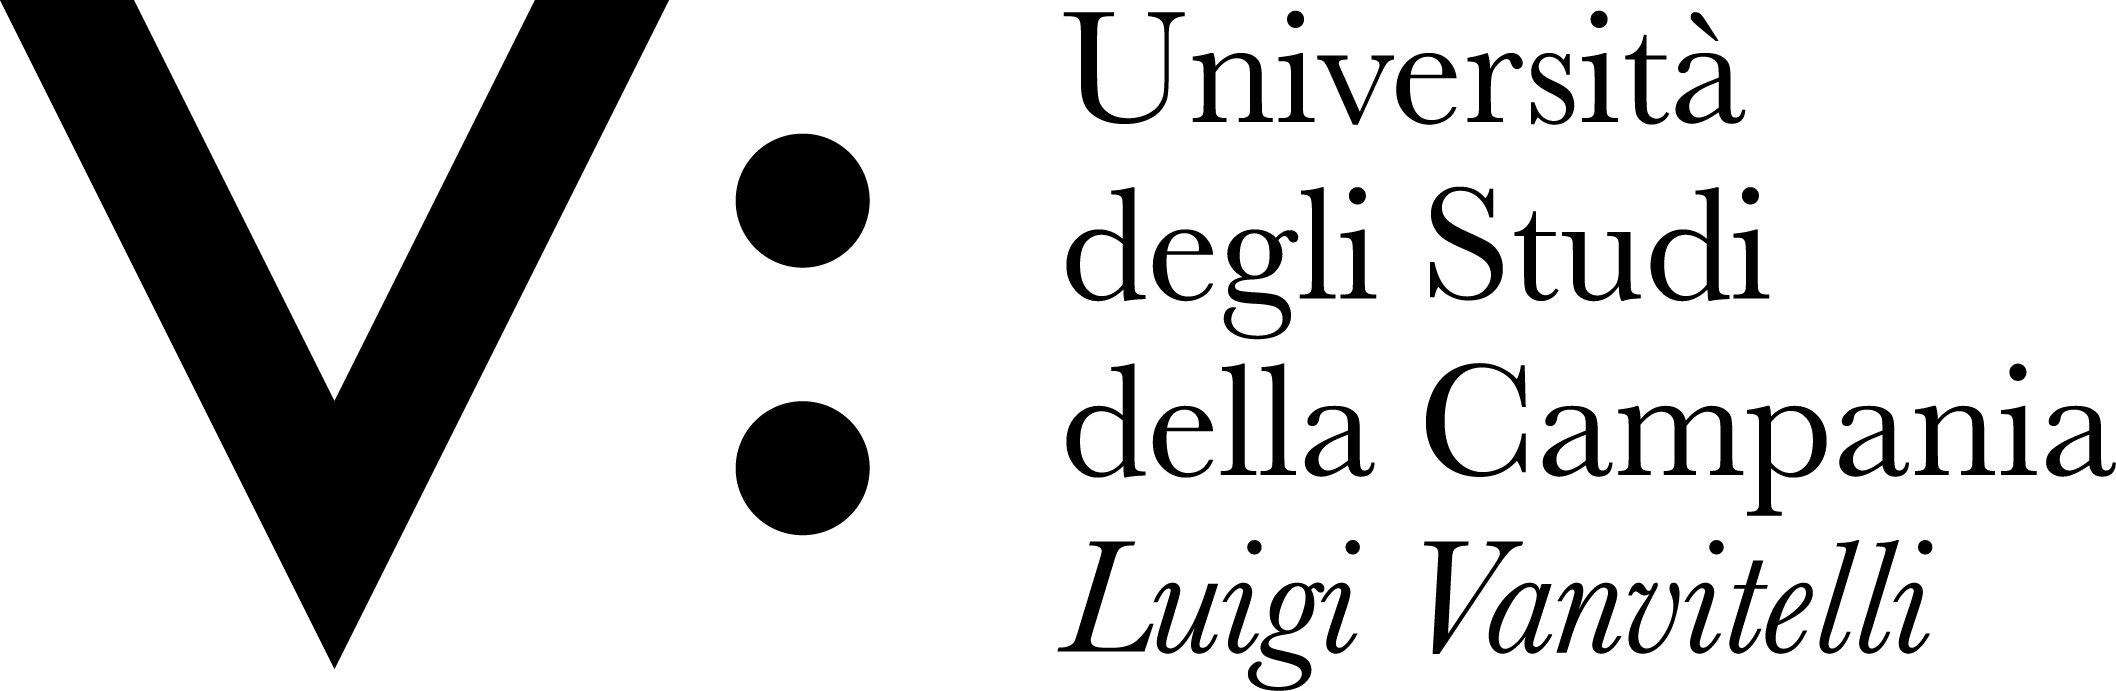
\includegraphics[scale=0.07]{logo} % University/department logo - uncomment to place it
 
%\vfill
\end{center}
\end{titlepage}

%----------------------------------------------------------------------------------------
%	DECLARATION PAGE
%----------------------------------------------------------------------------------------

\begin{declaration}
\addchaptertocentry{\authorshipname} % Add the declaration to the table of contents
\noindent I, \authorname, declare that this thesis titled, \enquote{\ttitle} and the work presented in it are my own. I confirm that:

\begin{itemize} 
\item This work was done wholly while in candidature for a research degree at \univname.
%\item Where any part of this thesis has previously been submitted for a degree or any other qualification at this University or any other institution, this has been clearly stated.
\item Where I have consulted the published work of others, this is always clearly attributed.
\item Where I have quoted from the work of others, the source is always given. With the exception of such quotations, this thesis is entirely my own work.
\item I have acknowledged all main sources of help.
%\item Where the thesis is based on work done by myself jointly with others, I have made clear exactly what was done by others and what I have contributed myself.\\
\end{itemize}
 
\noindent Signed:\\
\rule[0.5em]{25em}{0.5pt} % This prints a line for the signature
 
\noindent Date:\\
\rule[0.5em]{25em}{0.5pt} % This prints a line to write the date
\end{declaration}

\cleardoublepage

%----------------------------------------------------------------------------------------
%	QUOTATION PAGE
%----------------------------------------------------------------------------------------

\vspace*{0.2\textheight}

\noindent\enquote{\itshape 
By the love of God, the nations are created, and you love them like yourself. Love people as brothers, like freedom, then truth and life are for you. 
}
\bigbreak

\hfill  Abay Qunanbayev

%----------------------------------------------------------------------------------------
%	ABSTRACT PAGE
%----------------------------------------------------------------------------------------

\begin{abstract}
\addchaptertocentry{\abstractname} % Add the abstract to the table of contents

In this work, the following light weakly bound atomic nuclei are studied: $^6$He, $^6$Li and $^9$Be. 
A three-body model $\alpha$ + 2N for $^6$He and $^6$Li, and 2$\alpha$ + N model for $^9$Be are applied. 
The wave function of the three-body system is obtained within the framework of the Stochastic Variational Model based on the Gaussian basis. 
The interaction potentials for three-body systems have a Pauli projector, which excludes forbidden states. 
An analytical expression is obtained for the density distribution function of nuclear matter using the three-body wave function. 
The root-mean-square matter radii of the $^6$He, $^6$Li, $^9$Be nuclei are calculated and given comparisons with other sources.

The interactions of $^6$He, $^6$Li and $^9$Be with the simplest particles, such as $\alpha$, $d$ are studied in detail. 
On the basis of the calculated density distribution functions of the complex projectiles nuclear matter, the folding interaction potentials are obtained
%, and the comparison with global optical potentials are performed
. 
The resulting folding interaction potential is applied to calculate the differential cross sections of elastic scattering. 
Using the Coupled Channels approach for the $^9$Be induced reactions role  of different reaction channels is studied, and deformation parameters are derived. 
Comparisons of theoretical cross sections with experimental data in inelastic channels for nuclear reaction $d$ + $^9$Be $\rightarrow$ $d$ + $^9$Be$^*$ are given. 
Within the framework of the Coupled Reaction Channels method, the cross sections for nuclear reactions of single-nucleon and cluster transfers are calculated taking into account the internal structure of the $^6$He, $^6$Li and $^9$Be nuclei. 
%Features of the internal structure of these nuclei in direct nuclear reactions are manifested in their mechanism of transfer of clusters and nucleons. 
The mechanisms are revealed providing the contribution to the transfer of clusters and nucleons in the reactions induced by the $^6$He, $^6$Li and $^9$Be.

\end{abstract}

%----------------------------------------------------------------------------------------
%	ACKNOWLEDGEMENTS
%----------------------------------------------------------------------------------------

\begin{acknowledgements}
\addchaptertocentry{\acknowledgementname} % Add the acknowledgements to the table of contents
I believe that if it were not for these people, then the thesis in the form, in which you are reading it, would not have taken place.

I am very grateful to my scientific supervisors Prof. Nunzio Itaco and Prof. Andrey Denikin, who gave a great chance to implement my scientific ideas. Their suggestions, ideas and comments always gave me goals, raised my understanding of science higher and higher.

Undoubtedly, I think it is worthwhile to thank the staff of the Department of Physics and Astronomy and the CIRCE laboratory: Prof. D'Onofrio, Prof. Gialanella, Giuseppe Porzio, Liz, and all members.

In addition, I would like to express my gratitude to Prof. Vladimir Kukulin (Moscow Sate University), who gave advice on a scientific career, Prof Sayabek Sakhiyev (Abay State University), who gave not only scientific guides but also about life.

I also want to thank my dear friends Riccardo Mancino and Felice Pignatelli, without whom I could not just cope with simple life questions in Caserta.

Thanks to Prof. Ian Thompson (LLNL) for explaining the input file for the FRESCO code, Prof. Alexandr Volya (MSU), for providing the values of the spectroscopic amplitudes of alpha particles for p-shell nuclei.

I also dedicate my big thanks to my wife Mervet, who has always supported me at all stages of my scientific career, and my newborn daughter Dina, who has been a source of strength and positiveness.
\end{acknowledgements}

%----------------------------------------------------------------------------------------
%	LIST OF CONTENTS/FIGURES/TABLES PAGES
%----------------------------------------------------------------------------------------

\tableofcontents % Prints the main table of contents

\listoffigures % Prints the list of figures

\listoftables % Prints the list of tables

%----------------------------------------------------------------------------------------
%	ABBREVIATIONS
%----------------------------------------------------------------------------------------

\begin{abbreviations}{ll} % Include a list of abbreviations (a table of two columns)

NCSM & No Core Shell Model \\
RGM & Resonating Group Method \\
GCM & Generator Coordinate Method  \\
SVM & Stochastic Variational Method \\
DWBA & distorted wave Born approximation\\
CRC & coupled reaction channels \\
OM & optical model\\
DF & double folding\\
CC & coupled channel \\
SA & spectroscopic amplitude \\
cm & center of mass \\
rms & root-mean-square \\


\end{abbreviations}

%----------------------------------------------------------------------------------------
%	PHYSICAL CONSTANTS/OTHER DEFINITIONS
%----------------------------------------------------------------------------------------

\begin{constants}{lr@{${}={}$}l} % The list of physical constants is a three column table

% The \SI{}{} command is provided by the siunitx package, see its documentation for instructions on how to use it
%Constant Name & $Symbol$ & $Constant Value$ with units\\
Elementary electric charge & $e$ & 1.602 $\cdot~10^{-16}$ C \\
Reduced Planck constant & $\hbar$ & 6.582$ \cdot~10^{-16}$ eV$\cdot$s


\end{constants}

%----------------------------------------------------------------------------------------
%	SYMBOLS
%----------------------------------------------------------------------------------------

\begin{symbols}{lll} % Include a list of Symbols (a three column table)

%$P$ & power & \si{\watt} (\si{\joule\per\second}) \\
Symbol & Name & Unit \\

\addlinespace % Gap to separate the Roman symbols from the Greek

$r$ & distance & fm \\
$k$ & wavenumber & fm$^{-1}$ \\
$E$ & energy & MeV \\
$\rho(r)$ & density function  & fm$^{-3}$ \\
$A$ & atomic mass & u \\
$\sigma$ & cross section & mb\\
%$\Omega$ & angular frequency & \si{\radian} \\
${d \sigma \setminus d \Omega}$ & differential cross section & ${\rm{mb}}\setminus{\rm{sr}}$ 


\end{symbols}

%----------------------------------------------------------------------------------------
%	DEDICATION
%----------------------------------------------------------------------------------------

\dedicatory{to my mom \\~ \\ whom we had immeasurable love of mother and child\ldots} 

%----------------------------------------------------------------------------------------
%	THESIS CONTENT - CHAPTERS
%----------------------------------------------------------------------------------------

\mainmatter % Begin numeric (1,2,3...) page numbering

\pagestyle{thesis} % Return the page headers back to the "thesis" style

% Include the chapters of the thesis as separate files from the Chapters folder
% Uncomment the lines as you write the chapters

%\doublespacing

\chapter*{Introduction} % Main chapter title

\addchaptertocentry{Introduction}

Humanity has always been interested in the structure of the Universe - how it works, what it consists of. 
The understanding and naming of modern objects such as molecules and atoms began in ancient antiquity.
 The meaning of the word atom, in Greek $\alpha \tau o \mu o \varsigma$, is an indivisible, or uncut particle of matter. 
 Modern science has gone much deeper and determined that the atom is actually a complex particle. 
 According to the standard model, the fundamental particles are now six quarks, six leptons and their corresponding anti-particles and so on (for more details, see \cite{donoghue2014dynamics, griffiths2020introduction, ramond1999journeys}).  
All this is due to the development of integrated complex technology and detection systems designed to detect even the smallest details in fundamental interactions.
Particularly, in the modern nuclear physics the experimental techniques have also been successfully developed in the field of the production of secondary beams. 
Secondary beams, being rare and unstable nuclei, allow studying the properties and characteristics of the dripline nuclei, challenging the nuclear physics.

In recent years, the study of light weakly bound nuclei  has not lost interest due to the successful development of experimental facilities \cite{ter2004radioactive, yano2007riken, gade2016nscl, hong2014plan, fukuda2013identification}. 
It is known that in nuclei the nucleons tend to group into clusters. 
%A simple example that the cluster structure can be in heavy nuclei is the $\alpha$ decay of $^{238}$U, first experimentally discovered by Rutherford \cite{rutherford1899viii}. 
A well known manifestation of the cluster structure in heavy nuclei is the $\alpha$-decay of $^{238}$U, first experimentally discovered by E. Rutherford \cite{rutherford1899viii}. 
The $\alpha$-decay means that it can be formed in the uranium nucleus as an individual  subsystem.
The first quantitative theory of  $\alpha$-decay was developed by G. Gamov (see \cite{stuewer1986gamow}). In addition to $\alpha$-decay, there is also the cluster decay, where the emitted particle can be a heavy nucleus, for example -- $ ^ {12}$C \cite{poenaru2012cluster}.



There are many theoretical approaches \cite{descouvemont200112be, tohsaki2001alpha, kanada1995structure, pudliner1997quantum, zhukov1993bound}  devoted to studying the structure of exotic nuclei. In particular, the nuclear excitation function for light exotic nuclei is well reproduced by the No Core Shell Model (NCSM) method \cite{navratil2009recent, forssen2005large, navratil2003ab, navratil2002ab}. 
The method uses one-particle basis function of the harmonic oscillator,  realistic NN, NNN interactions. 
This method is reduced to solving the $A$-nucleon Schr\"{o}dinger equation on a basis containing all possible configurations of $A$-nucleon oscillator functions. 
However, the size of the basis grows rapidly with the number of nucleons, the reliability of the NCSM model calculations decreases in the case of heavy nuclei. At present, the capabilities of modern computational machines make it possible to calculate with sufficient accuracy of nuclei with masses $A \le 16$.
For example, in Ref. \cite{forssen2005large} within the framework of this model, the excitation spectrum of the one-particle basis for the \be nucleus is in good agreement with the experimental data. 

The microscopic description, that is, taking into account the NN effective potential, of the break-up reaction was presented in the Resonating Group Method (RGM) \cite{horiuchi1970generator, tang1978resonating, wheeler1937mathematical}. Generalization of the RGM consists in constructing overall mathematically equivalent methods for the simultaneous calculation in the nuclear structures and nuclear reactions. 
The practical application of this method is also limited in the region of the lightest nuclei due to the lack of computational power in the antisymmetrization process.
In the work \cite{nesterov2010three} the algebraic RGM was successfully applied in describing the internal structure \he, \li and $^8$He nuclei, calculated their rms matter and proton
and neutron radii, as well as nuclear matter distribution density. Also the fusion reactions at low energies participating \he were presented.

Similar to the RGM \cite{horiuchi1970generator}, is the Generator Coordinate Method (GCM), if one takes the full model space of the basis Bloch-Brink wave functions \cite{brink1966proceedings}. 
In the framework of the GCM it is possible to carry out calculations for the nuclei with medium masses implementing many clusters. 
For scattering problems, the RGM can be applied rather straightforwardly because the inter-cluster wave function is explicitly treated. On the other hand, in the application of the GCM to scattering problems, it is necessary to connect the basis wave functions in the internal region with continuum states in the asymptotic region at a chosen channel radius \cite{descouvemont2010r}. 
 Microscopic three-body calculations for two valence neutrons around a core nucleus have been achieved by many groups to investigate the neutron halo and two-neutron correlation in drip-line nuclei such as \he and $^{14}$Be \cite{arai1999structure, descouvemont1995halo}. 
 The $^{12}$Be using the GCM has been studied \cite{descouvemont200112be}. 
 In this work a negative-parity band was found, electromagnetic transition probabilities and partial widths of molecular states were calculated.
 

In addition to the above theoretical approaches, there is the Stochastic Variational Method (SVM) \cite{kukulin1977stochastic, voronchev1994study, kukulin1986detailed, kukulin1984detailed}. 
The SVM uses the Gaussian function as a basis function, which is convenient for analytical deriving matrix elements of the Hamiltonian. 
The corresponding Hamiltonian contains a Pauli projector \cite{kukulin1978orthogonal}, that removes forbidden states. 
The variational method describes well the internal structures of \he, \li and \be \cite{kukulin1984detailed, kukulin1986detailed, voronchev1994study}. 
In particular, the electromagnetic properties, geometric parameters and configuration weights are in good agreement with the methods, where they are obtained by real solutions of three-body problems. 

To describe the elastic scattering in the field of a complex potential, one usually uses the Optical Model (OM), first presented in Ref. \cite{feshbach1958optical}. Within the framework of this model, the nucleus is considered as a transparent substance that has the ability to absorb. In practice, this method describes the experimental data well providing the direct information on the nucleus-nucleus interaction potential.
However, the ambiguity of the optical potential parameters reduces the merits of optical model.
To study the inelastic channels, transfer reactions and their use to describe experimental data the Distorted Wave Born Approximation (DWBA) method has been successfully applied \cite{satchler1960gamma}.
The DWBA method proved to be appropriate and successful in describing the cross section of nuclear reactions involving ground and low-lying excited nuclear states of single particle type as well as collective nature.
The method becomes inadequate, since the reaction leads to the broad or strongly overlapped final states.
In this case the couples channel formalism has to be applied.

\begin{figure}
\centering
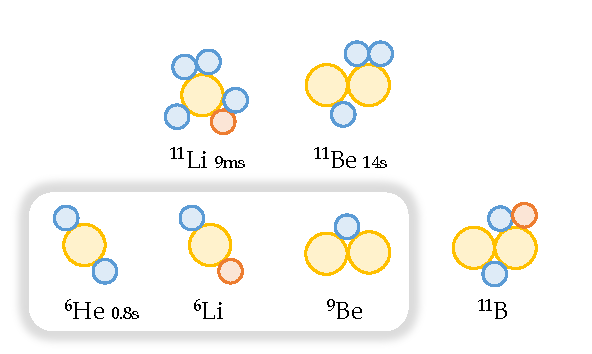
\includegraphics[scale=1]{exotic_nuclei}
\decoRule
\caption{\footnotesize Schematic representation of the cluster structure of some nuclei, and their half-life, if unstable. Alpha particle, proton and neutron are marked in yellow, red and orange, respectively. The allocation of \he, \li and \be nuclei means the selected as objects of study. Read the text for more details..}
\label{fig:exotic_nuclei}
\end{figure}

In light nuclei, the cluster structure can often be clearly manifested in the dripline region of the nuclear map. 
These series include such nuclei as \he, $^{11}$Li, $^{12}$Be and other exotic nuclei. 
However, there are also stable nuclei with prominent cluster structures. These include such nuclei as \li, \be, $ ^{11}$B and others. Numerous experimental data \cite{canto2006fusion, brown2007, papka2007} allow us to treat such nuclei as multi-cluster systems, including tightly bound $\alpha$-clusters and valence nucleons. A visual representation of how these nuclei are arranged in the cluster model is illustrated in Fig \ref{fig:exotic_nuclei}. 
For these nuclei the relative motion of internal subsystems determines the property and mechanisms of nuclear reactions. 
In the figure, we see that the simplest nuclei with a cluster structure are \he, \li and \be. 
Their structure is ideally suited to consideration within the framework of the three-body model. 
The model has well-known many works on the theoretical approach. 
Moreover, it should be noted that the interaction of pairs inside these nuclei is also well known, which can be used in constructing a solution to the Schr\"{o}dinger equation. An important factor is also the number of scattering experiments made to study these nuclei.
Therefore, the objects of studying in this work have been taken the \he, \li and \be nuclei.

Elastic scattering of the \he + $\alpha$  and \li + $\alpha$ data is available at laboratory energies 151 MeV and 166 MeV \cite{ter1998two, oganessian1999dynamics}. 
This experimental data are candidates for showing the elastic transfer phenomenon through two-neutron transfer between the two $\alpha$ core. The main motivation of these studies was to probe the relative importance of the "di-neutron" and "cigar" configurations of the valence neutrons in the \he ground state. 
The data sets show the backward angle rise in cross section.
Usually it is considered characteristic of elastic transfer. 
The DWBA analysis using the \he and \li wave functions built on hyper-spherical harmonics \cite{zhukov1993bound}, obtained good agreement with the backward angle data.
Consequently, it is concluded that the di-neutron configuration dominates the \he ground state wave function.
The more detailed study of the \he + $\alpha$ scattering data has carried out in Ref. \cite{khoa2004di} in the framework of the Coupled Reaction Channels (CRC) method. 
In this work the spectroscopic information of the di-neutron was obtained, a sequential transfer of the di-neutron was implemented in CRC calculations. It was concluded that the two valence neutron are transferred mainly simultaneously, the rising at backward angles comes due to the elastic transfer of the $2n$ cluster. 


%Scattering of the simplest projectiles, such as ${}^{1,2}$H or ${}^{3,4}$He, off a target is a standard tool for fundamental study of the structure of nuclei. This method involves measuring the angular distributions of the nuclear reaction products. It is well known that the energies and angular distributions of projectile-like particles give information about the internal structure of target-like nuclei. 
%In the works \cite{lukyanov2014, lukyanov2015, janseitov2018}, the ${}^3$He interaction with ${}^9$Be was studied and angular distributions of the reaction products were measured.
% in the following exit channels: ${}^3$He+$^9$Be, ${}^5$He+$^7$Be, ${}^5$Li+$^7$Li, ${}^6$Be+$^6$He, and ${}^6$Li+$^6$Li, were measured. 
%The obtained data were analysed within the framework of the optical-model (OM), the coupled-channel (CC) and the distorted-wave Born approximation (DWBA) approaches. The performed analysis of the experimental data showed sensitivity of the cross sections on the potential parameters in the exit channels. 
%These experiments were designed to study the breakup reactions with ${}^9$Be in an attempt to determine contributions of the channels with the ${}^8$Be+n  and  ${}^5$He+$\alpha$ structure to the inclusive measurements. It was found that these two channels contribute in the ratio of 2.7~to~1, respectively. The determined value justifies that the ${}^5$He+$\alpha$ breakup channel plays an important role as well.

Based on the Borromean structure of ${}^9$Be, special attention was focused on the breakup processes resulting from the ${}^9$Be($^6$Li, ${}^6$Li$^\prime$)$^9$Be$^*$ nuclear reaction \cite{brown2007, papka2007}. The excited nucleus ${}^9$Be$^*$ can decay either directly into the $\alpha+\alpha+n$ three-body system or through one of the unstable nuclei, such as ${}^5$He and ${}^8$Be. These relatively recent experimental studies explicitly confirm the cluster structure of ${}^9$Be.
The calculated branching ratios show that the low-lying excited states, at E$_x <$~4.0 MeV, are mostly populated with the ${}^8$Be+n configuration. In other conditions, the ${}^5$He+$\alpha$ configuration plays a significant  role.
Another aspect of finding the cluster structure is its  effect on the nuclear reaction mechanisms. Indeed, since the papers \cite{detraz1970, detraz1974}, the multi-particle-multi-hole structures have been expected at rather low excitation energies in nuclei. In such a case, it can be understood that the correlated nucleons are transferred as a whole strongly correlated cluster, which has the internal quantum numbers of a free particle.

In the present work, the three-body structure of nuclei and their role in the mechanisms of nuclear reactions are investigated.
 Usually, in the descriptions of the cross sections for nuclear reactions, the intrinsic structure of colliding nuclei in the interaction potentials is neglected, taking them in a phenomenological way. 
 For example, in Gaussian form, or in the form of the Woods-Saxon potential \cite{oganessian1999dynamics}.
 In such cases, one should take the potential corresponding to realistic shapes of colliding nuclei.
 To describe direct nuclear reactions, we proceed from realistic shape of colliding nuclei within the three-body model.
 Therefore, the motivation for this work is to minimize the number of free parameters in the calculations of nuclear reactions as much as possible, and to use the densities distribution functions of nuclear matter based on the three-body model. And also the main goal of this work is to understand how the mechanisms of interaction of nuclear reactions with the participation of the weakly bound nuclei \he, \li and \be occur. 

This work is organized as follows. The first chapter is devoted to an introduction to the three-body model based on the SVM method. This chapter details the advantage of using the Gaussian basis function, the Hamiltonian, which includes the Pauli principle, the transformation of the basis function, and provides formulas for calculating the density function of nuclear matter within the three-body model. 
The next chapter presents widely used theoretical approaches to describe the scattering wave function. 
Methods for calculating differential cross sections  are presented. For elastic scattering -- Optical model, inelastic scattering -- Coupled channel, and nuclear transfer reactions -- Coupled Reactions Channels. 
For a complete understanding of how one-particle spectroscopic amplitudes (SA) are calculated within the framework of the shell model used in CRC calculations, a separate section is devoted.
Details of building the potential of interaction in the framework of double folding are presented.
The last third chapter presents the results of calculations. 
In this chapter the geometric structure of the obtained three-body wave function is illustrated. 
The density distribution functions of nuclear matter for the \he, \li and \be nuclei are presented in the framework of a three-body model. 
Comparisons of the calculated differential cross sections with experimental data for the elastic scatterings, \he + $\alpha$ at the laboratory energy 151 MeV  and \li + $\alpha$ at 166 MeV, are given. 
%A detailed analysis of the interaction of deuteron with the nucleus of \be is given.
The next section is devoted to the investigation of the cluster structure of the ${}^9$Be nucleus through studying the nuclear reactions caused by a deuteron beam at 19 MeV and 35 MeV incident energies. 
A comparative analysis of experimental data and theoretical calculations has been performed.
Finally, the main finding are presented in the conclusion.

\label{Chapter1} % For referencing the chapter elsewhere, use \ref{Chapter1} 

%----------------------------------------------------------------------------------------

% Define some commands to keep the formatting separated from the content 
\newcommand{\keyword}[1]{\textbf{#1}}
\newcommand{\tabhead}[1]{\textbf{#1}}
\newcommand{\code}[1]{\texttt{#1}}
\newcommand{\file}[1]{\texttt{\bfseries#1}}
\newcommand{\option}[1]{\texttt{\itshape#1}}

%----------------------------------------------------------------------------------------

\chapter{The three body model}
The wave function for the three-body system in the current work was calculated within the model proposed in Ref. \cite{kukulin1977stochastic}.
 The work based on the three body model provides great progress in understanding the structure and properties of the light weakly bound nuclei, like $^6$He, $^6$Li, $^9$Be nuclei. 
 In addition, a lot of research has been done in different directions of physics \cite{kukulin1977stochastic, golovkov1981cross, kukulin1984detailed, glozman1984study, kukulin1986detailed, voronchev1994study, zhusupov1994elastic, kukulin2010, seksembayev2018, kakenov2020properties} using this wave function. Below we list some of them:
\begin{itemize}
\item electromagnetic properties;
\item  low lying excitation spectra;
\item root-mean-square charge radii $\langle r_{ch}^2\rangle^{1/2}$,  magnetic $\mu$, quadrupole $Q$ and octupole $\Omega$  moments;
\item processes of $^6$Li interaction with hadrons, including quasi-elastic scattering ($ \alpha $, 2$\alpha $), ($ p $, $ d $) and ($p$, $p\alpha$);
\item high energy proton and the lightest nuclei scattering on $^6$Li
\item scattering of $\pi^{\pm}$-mesons and $\mu$-capture by $^6$Li
\item parameters of $\beta$-decay of $^6$He;
\item the thermonuclear reactions in the D-$^3$He-$^9$Be plasma;
\item properties of the six-quark dibaryons in nuclei with $A$=6 and \textit{etc}.
\end{itemize}
Since this wave function was widely used, we chose it as the wave function to describe the three-body system in this work.



\section{Basis function}
Consider the three body system containing a boson $k$ and two fermions, $p$ and $q$. 
 A total wave function of this system with total spin $ J $ and spin projection $ M $ can be represented as
 \begin{equation}
 \Psi^{JM}_{tot}
 = \psi\left( k \right) 
 \Psi^{JM}\left( {\bf x}_k, {\bf y}_k \right).
 \label{totwf}
 \end{equation}
Here, $\psi\left( k \right)$ -- internal wave function of the $k$-particle, $\Psi^{JM}\left( {\bf x}_k, {\bf y}_k \right)$ -- wave function of the relative motion depending on the Jacobi coordinates $ {\bf x}_k $ and $ {\bf y}_k $. The vector $ {\bf x}_k $ is a vector of the relative distance between the pair of particles $ pq $ and $ k $, and $ {\bf y}_k $ is the vector of the relative distance between the center of mass of the pair $ pq $ and the particle $ k $ (see Fig. \ref{fig:jacobiSet}). The wave function of relative motion may be expanded into a components as
\begin{equation}
\Psi^{JM}\left( {\bf x}_k, {\bf y}_k \right)=\sum_\gamma\Psi^{ J M}_\gamma\left( {\bf x}_k, {\bf y}_k \right),
\end{equation}
where  $\gamma \equiv \{\lambda l L S\}$.
The momenta $ \lambda $, $ l $ are the orbital momenta conjugated to the coordinates $ {\bf x} _k $ and $ {\bf y} _k $ respectively, $ L $ is the total orbital momentum of the system and $S$ is the total spin of the pair $pq$.  
The each component defines spatial and spin parts as follow
\begin{align}
\Psi^{ J M}_\gamma\left( {\bf x}_k, {\bf y}_k \right) = & \left[
\Phi^{(\lambda,l)}_L \left({\bf x}_k, {\bf y}_k \right) \otimes
\chi_S(pq)
\right]_{JM} =  \\
=& 
\sum_{M_L M_S} (LM_LSM_S | JM) ~
\Phi^{(\lambda,l)}_{LM_L}\left( {\bf x}_k, {\bf y}_k \right)~
\chi_{SM_S}(pq) \nonumber
\end{align}
The spin function of the pair ($pq$) is given by
\begin{equation}
\chi_{SM_S}(pq)=\left[ \chi_{\tfrac{1}{2}}(p) \otimes \chi_{\tfrac{1}{2}}(q)	\right]_{SM_S}.
\end{equation}
The spatial part of the wave function is chosen to be multidimensional Gaussian functions of the form
\begin{align}
\Phi^{(\lambda,l)}_{LM_L} \left({\bf x}_k, {\bf y}_k \right)=&
x^\lambda y^l 
\sum_i C_i 
\exp\left( - \alpha_i^{(k)} x^2_k - \beta_i^{(k)} y^2_k \right)~
\times \nonumber \\
& \times \left[ 
Y_\lambda \left(\hat{x}_k \right) \otimes Y_l \left(\hat{y}_k \right)
\right]_{LM_L}.
\label{spatial_part}
\end{align}
Here, the coefficients $ C_{i} $ are the parameters of the wave function expansion and are found as a result of solving the generalized eigenvalue problem. 
The linear parameters  $ \alpha^{(k)} _ {i} $, $ \beta^{(k)}_{i}$ 
make the wave function more complete, if they are represented in the following form
\begin{align}
\alpha^{(k)} _ {i} =& \alpha_0~ \tan 
\left( \frac{\pi}{2} \frac{2i-1}{2N_{\gamma}} \right),
  \\
\beta^{(k)} _ {i} =& \beta_0~  \tan 
\left( \frac{\pi}{2} \frac{2i-1}{2N_{\gamma}} \right),
~~~ i=1,~...,~N_{\gamma}.
\end{align}
Finally, the basis function for the three body system $(k,~pq)$ can be represented in form 
\begin{align}
\phi^{ J M}_{\gamma i} \left(k, pq \right)=
C_i \psi \left( k \right) 
 \varphi^{(\lambda,l)}_i(x_k,y_k) \left[ \left[ 
Y_\lambda \left(\hat{x}_k \right) \otimes Y_l \left(\hat{y}_k \right)
\right]_{L} \otimes \chi_S (pq) \right]_{JM}.
\label{basis_function_1}
\end{align}
Here, the coordinate arguments, ${\bf x}_k$ and ${\bf y}_k$,   are down for convenience, and the radial part of the basis function has form
\begin{equation}
\varphi^{(\lambda,l)}_i(x_k,y_k)=
  x^\lambda y^l \exp\left( - \tfrac{1}{2} \alpha_i^{(k)} x^2_k - \tfrac{1}{2} \beta_i^{(k)} y^2_k \right)
\end{equation}

\begin{figure}[b]
\centering
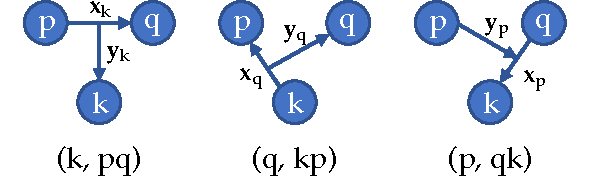
\includegraphics[scale=1.0]{pic1}
\decoRule
\caption{\footnotesize The schemes of Jacobi coordinate sets for the three body system.}
\label{fig:jacobiSet}
\end{figure}

If the three body system consisted of a fermion $k$ and two boson $(pq)$, the total wave function (\ref{totwf}) may be rewritten as follows:
\begin{equation}
\Psi^{JM}_{tot} 
 = \psi\left( p \right) 
 \psi\left( q \right) 
 \Psi^{JM}\left( {\bf x}_k, {\bf y}_k \right),
\end{equation} 
where $\psi\left( p \right)$ and $\psi\left( q \right) $ -- internal wave functions of the $p$ and $q$ particles correspondingly.
The wave function of relative motion $\Psi^{JM}\left( {\bf x}_k, {\bf y}_k \right)$ has the similar form, except the spin part $\chi(k)_{\tfrac{1}{2}m_s}$. Thus, the basis function for the three body system having only one fermion $k$ can be expressed as
\begin{align}
\phi^{ J M}_{\gamma i} \left(k, pq \right)=
\psi\left( p \right) 
 \psi\left( q \right) 
\varphi^{(\lambda,l)}_i(x_k,y_k) 
 \left[ \left[ 
Y_\lambda \left(\hat{x}_k \right) \otimes Y_l \left(\hat{y}_k \right)
\right]_{L} \otimes \chi(k)_{\tfrac{1}{2}} \right]_{JM}.
\label{basis_function_2}
\end{align}

A pair of the three body system may have forbidden states according to the principle Pauli. 
For instance, lets say, the pair $(kp)$ has the state $f$ must be excluded.  
This forbidden state $f$ is projected out by implementing the pseudo-potential \cite{kukulin1978orthogonal}:
\begin{equation}
\label{pseudopot}
\widetilde{V}_{kp}=V_{kp}+\lambda \Gamma_f,
\end{equation}
where $V_{kp}$ is  a regular interaction potential between $p$ and $k$ particles,  $\lambda$ -- a constant usually equal to $10^5$. The operator $\Gamma_f$ is given by:
\begin{equation}
\label{projector}
\Gamma(f)=~
\sum\limits_{m_f}\vert \phi_{fm_f} ({\mathbf x})\rangle~ 
 \langle  \phi_{fm_f} ({\mathbf x'}) \vert ~
 \delta({\mathbf y - \mathbf y'}).
\end{equation}
So the three body Hamiltonian including kinetic energy and pseudo potentials looks as
\begin{equation}
\label{pseudohamiltonian}
H=H_0+\sum_{k < p} \widetilde{V }_{kp}.
\end{equation}

The Pauli principle plays a huge role in the structure of the nucleus, particularly it does not allow overlapping of two constituent particles, while maintaining the Paili principle.
This approach, so-called the method of orthogonalizing pseudo-potentials, was previously developed by the group of V. Kukulin \cite{kukulin1978orthogonal}, and is widely used not only in the construction of the wave function of the bound state, but also in the scattering theory \cite{blokhintsev1993determination, tursunov2016theoretical}.

 \section{Transformation of the basis function }
The main advantage of the basis functions,  (\ref{basis_function_1}) and (\ref{basis_function_2}), is in simplicity of transformation into an alternative set of Jacobi coordinates \cite{suzuki1998stochastic}.
The transformation from the sets $(k,pq)$ to $(q,kp)$ may be accomplished as follows:
\begin{equation}
\begin{pmatrix}
{\bf x}_k \\ 
{\bf y}_k
\end{pmatrix}  = {\bf T}^{(kq)}
\begin{pmatrix}
{\bf x}_q \\ 
{\bf y}_q
\end{pmatrix},
\end{equation}
where, the ${\bf T}^{(kq)}$ matrix elements is given by  
\begin{equation}
{\bf T}^{(kq)} = 
 \begin{pmatrix}
 {\rm T}^{(kq)}_{11} & {\rm T}^{(kq)}_{12} \\
 {\rm T}^{(kq)}_{21}  &  {\rm T}^{(kq)}_{22}
 \end{pmatrix}.
\end{equation}
In this work the transformation matrices ${\bf T}^{(kq)}$ and ${\bf T}^{(kp)}$ are mostly used. Therefore, the matrix ${\bf T}^{(kp)}$ can be expressed as
\begin{equation}
{\bf T}^{(kp)} = 
 \begin{pmatrix}
 -\tfrac{m_k}{m_q+m_k} & -1 \\
-\tfrac{m_q(m_k+m_p+m_q)}{(m_q+m_k)(m_p+m_q)}  & -\tfrac{m_p}{m_p+m_q}
 \end{pmatrix}
\end{equation}
 and the matrix ${\bf T}^{(kq)}$ has form
 \begin{equation}
{\bf T}^{(kq)} = 
 \begin{pmatrix}
 -\tfrac{m_k}{m_k+m_p} & 1 \\
-\tfrac{m_p(m_k+m_p+m_q)}{(m_k+m_p)(m_p+m_q)}  & -\tfrac{m_q}{m_p+m_q}
 \end{pmatrix}.
\end{equation}
%There is no need to consider the transformation of spin part of the basis function. The reason is that the $S$ spin of the $2\alpha+n$ three-body system is defined only by the vacant nucleon, and it doesn't depend on the choice of the Jacobi coordinate. That is to say, the coupling of the vacant nucleon spin with the $\alpha-\alpha$ subsystem spin gives again the spin of the nucleon due to the $\alpha$ particles having a spin of zero.  

The transformation of the spatial part (\ref{spatial_part}) of the wave function can be expressed in the following way \cite{suzuki1998stochastic, kukulin1990dynamic}

  \begin{equation}
 \label{transform_spatial_part}
 \Phi^{(\lambda,l)}_{LM_L}\left( {\bf x}_k, {\bf y}_k \right) = \sum_{\tilde{\lambda}, \tilde{l}} A^{\tilde{\lambda} \tilde{l} \lambda l}_{{\bf T}^{(kq)} }~
  \Phi_{LM_L}^{(\tilde{\lambda},\tilde{l}) } \left(  {\bf x}_q, {\bf y}_q \right) ,
 \end{equation}
where the summation is proceeded over new quantum numbers $\tilde{\lambda},~\tilde{l}$ in condition $\lambda+l=\tilde{\lambda}+\tilde{l}$, and the new spacial part is given by
\begin{align}
 \Phi_{LM_L}^{(\tilde{\lambda},\tilde{l}) } \left(  {\bf x}_q, {\bf y}_q \right)  =  &
x^{\tilde{\lambda}}_q y^{\tilde{l}}_q 
\sum_{i=1}^{N_\gamma} C_i 
\exp\left( - \tfrac{1}{2} \alpha_i^{(q)} x^2_q -\tfrac{1}{2}  \beta_i^{(q)} y^2_q 
- \rho_i^{(q)}   {\bf x}_q \cdot {\bf y}_q 
   \right)~
\times \nonumber \\
& \times \left[ 
Y_{\tilde{\lambda}} \left(\hat{x}_k \right) \times Y_{\tilde{l}} \left(\hat{y}_k \right)
\right]_{LM_L}.
\label{new_spacial_part}
\end{align}
%, !taking into account the condition $ \tilde{\lambda} + \tilde{l} = \lambda + l $!.
where new linear parameters can be expressed as
\begin{align}
\begin{pmatrix}
\alpha_i^{(q)} & \rho_i^{(q)} \\ 
\rho_i^{(q)} & \beta_i^{(q)}
\end{pmatrix}  = \left( {\bf T}^{(kq)} \right)^{T} \times  ~
\begin{pmatrix}
\alpha_i^{(k)} & \rho_i^{(k)} \\ 
\rho_i^{(k)} & \beta_i^{(k)}
\end{pmatrix} ~ \times
  {\bf T}^{(kq)}.
\end{align}
%\nonumber \\
%\alpha^{(q)}_{i} =& \alpha^{(k)}_{i} T_{11}^2 + \beta^{(k)}_{i} T_{21}^2 
%\nonumber \\
%\beta^{(q)}_{i} =& \alpha^{(k)}_{i} T_{12}^2 + \beta^{(k)}_{i} T_{22}^2 
%\nonumber \\
%\rho^{(q)}_{i} =& 2 \alpha^{(k)}_{i} T_{11} T_{12} + 2 \beta^{(k)}_{i} T_{21}  T_{22} 
Note, that for the initial  coordinate set $(k,pq)$ the radial wave function (\ref{spatial_part}) does not include the scalar product ${\bf x}_k \cdot {\bf y}_k$, which means $\rho_i^{(k)}=0$.  

The coupling coefficient $A^{\tilde{\lambda} \tilde{l} \lambda l}_{{\bf T}^{(kq)} }$  given in ~(\ref{transform_spatial_part}) is defined as follows
 \begin{align}
 A^{\tilde{\lambda} \tilde{l} \lambda l}_{{\bf T}^{(kq)} } = & \sum_{\lambda_1 \lambda_2 l_1 l_2} 
\left({\rm T}_{11}^{(kq)} \right)^{\lambda_1} 
\left({\rm T}_{12}^{(kq)} \right)^{\lambda_2} 
\left({\rm T}_{21}^{(kq)} \right)^{l_1} 
\left({\rm T}_{22}^{(kq)} \right)^{l_2} 
\times \nonumber
\\
& \times {E}^{\lambda_1 \lambda_2 \lambda l_1 l_2 l L}_{\tilde{\lambda} \tilde{l} } \mathcal{D}(\lambda,\lambda_1,\lambda_2) \mathcal{D}(l,l_1,l_2).    
\label{trans_coef}
\end{align}
Here, the summation is satisfied to the conditions $\lambda_1+\lambda_2=\lambda$, $l_1+l_2=l$, $\lambda+l=\tilde{\lambda}+\tilde{l}$, the coefficients ${E}^{\lambda_1 \lambda_2 \lambda l_1 l_2 l L}_{\tilde{\lambda} \tilde{l} }$ and $\mathcal{D}(\lambda,\lambda_1,\lambda_2)$ come from re-coupling of the solid spherical harmonics , which are given in Appendix \ref{AppendixA}. Switching into the Jacobi set $(p,qk)$ is carried out in analogous way.

The spin part $\chi_{SM_S}(pq)$ of the wave function transforms as
\begin{equation}
\chi_{SM_S}(pq) = (-1)^{s_p+s_q-S} \chi_{SM_S}(qp).
\end{equation}
As for the one fermionic system the spin part remains unchanged.

\section{Overlap matrix elements}
The overlap matrix elements for the basis function (\ref{basis_function_1}) is expressed as follows
\begin{align}
\langle \phi^{ J M}_{\gamma i}\left(k, pq \right) \vert 
\phi^{ J M}_{\gamma^{\prime}j}\left(k, pq \right) \rangle=&
 \int \int d{\bf x}_k d{\bf y}_k 
 ~\phi^{ J M}_{\gamma i}\left(k, pq \right) 
 \left( \phi^{ J M}_{\gamma^{\prime} j}\left(k, pq \right) \right)^{*}
 = \label{overlap_in_basic_set}
\\ 
=\int_0^\infty \int_0^\infty  dx_k dy_k~ & x_k^{2\lambda+2}y_k^{2 l +2} {\rm exp}\left( - \tfrac{1}{2}\alpha^{(k)}_{ij} x^2_k - \tfrac{1}{2} \beta^{(k)}_{ij} y^2_k \right) \delta_{\gamma \gamma'} =
 \nonumber \\ 
=&~ 
 C_i C_j
\mathcal{I} \left( 2\lambda+2,\alpha_{ij}^{(k)} \right)~ \mathcal{I} \left(2l+2,\beta_{ij}^{(k)} \right) ,\nonumber
\end{align} 
where
$
\alpha_{ij}^{(k)}=\alpha_{i}^{(k)}+\alpha_{j}^{(k)}$ and $
\beta_{ij}^{(k)}=\beta_{i}^{(k)}+\beta_{j}^{(k)}
$,
the table integral $\mathcal{I}(\lambda, \alpha)$ is  
\begin{equation}
\mathcal{I} \left( \lambda,\alpha\right)=
 2^{1+\lambda}\frac{\Gamma \left( 1+\lambda \right)  }{ \left( \alpha \right) ^{1+\lambda}} .
\label{table_integral_1}
\end{equation}

It is also useful to give an expression of overlap matrix elements for alternative Jacobi coordinate set. For instance, the matrix elements for the $(q,kp)$ three body system may be given as follows
\begin{equation}
\langle \phi^{ J M}_{\gamma i}\left(k,pq \right) \vert 
\phi^{ J M}_{\gamma^{\prime}j}\left(k,pq \right) \rangle
=
\sum_{\tilde{\gamma} \tilde{\gamma}'}
A^{\tilde{\lambda}' \tilde{l}' \lambda' l'}_{{\bf T}^{(kq)} }
A^{\tilde{\lambda} \tilde{l} \lambda l}_{{\bf T}^{(kq)} }
\langle \phi^{ J M}_{\tilde{\gamma}i}\left(q,kp \right) \vert 
\phi^{ J M}_{\tilde{\gamma}^{\prime}j}\left(q,kp \right) \rangle
\label{overlap_alternative}
\end{equation}
The Jacobian  matrix ${\bf J}^{(kq)}$ for transformation from the ${\bf x}_k, {\bf y}_k$ coordinates to the ${\bf x}_q, {\bf y}_q$ coordinates gives the ${\bf T}^{(kq)}$ matrix
\begin{equation}
{\bf J}^{(kq)} = 
\begin{pmatrix}
\frac{\partial {\bf x}_k \left({\bf x}_q,{\bf y}_q \right)}{ \partial {\bf x}_q }  
& \frac{\partial {\bf x}_k \left({\bf x}_q,{\bf y}_q \right)}{ \partial {\bf y}_q } \\
\frac{\partial {\bf y}_k \left({\bf x}_q,{\bf y}_q \right)}{ \partial {\bf x}_q }  
& \frac{\partial {\bf y}_k \left({\bf x}_q,{\bf y}_q \right)}{ \partial {\bf y}_q } 
\end{pmatrix} = {\bf T}^{(kq)}.
\end{equation}
Accordingly, the determinant $\vert {\bf J}^{(kq)} \vert$ is a determinant of the ${\bf T}^{(kq)}$ matrix, which equals to $1$:
\begin{equation}
\vert {\bf J}^{(kq)} \vert = \vert {\bf T}^{(kq)} \vert =1.
\end{equation}
  Therefore, the integration variables in Eq.~(\ref{overlap_alternative}) can be changed without any factorization. 

The spacial part (\ref{new_spacial_part}) in the alternative coordinate set has the scalar product, $\exp \left(- \alpha_i^{(q)} \beta_i^{(q)}  {\bf x}_q \cdot {\bf y}_q  \right)$. With this form the overlap matrix elements can be calculated directly, using the expansion of the exponential function \cite{suzuki1998stochastic}. However it is possible  to project the scalar product into ${\bf T}$ matrix \cite{kukulin1990dynamic} as follows:
 \begin{equation}
{\bf Q}_i^{(kq)}= {\bf T}^{(kq)} \times
\begin{pmatrix}
1 &  0 \\ 
-\tfrac{\rho^{(q)}_{i}}{\alpha^{(q)}_i} & 1
\end{pmatrix} .
\label{q_rotation_matrix}
\end{equation}
Consequently, the radial part (\ref{new_spacial_part}) of the wave function can be rewritten without the scalar product term as
\begin{align}
 \Phi_{LM_L}^{(\tilde{\lambda},\tilde{l}) } \left(  {\bf x}_q, {\bf y}_q \right)  =  &
x^{\tilde{\lambda}}_q y^{\tilde{l}}_q 
\sum_{i=1}^{N_\gamma} C_i 
\exp\left( - \tfrac{1}{2} 
{\alpha'}^{(q)}_{i}
 x^2_q -\tfrac{1}{2}  \beta_i^{(q)} y^2_q \right)
\times \nonumber \\
& \times \left[ 
Y_{\tilde{\lambda}} \left(\hat{x}_k \right) \times Y_{\tilde{l}} \left(\hat{y}_k \right)
\right]_{LM_L}.
\label{new_spacial_part}
\end{align}
with 
\begin{equation}
{\alpha'}^{(q)}_{i}=
\alpha^{(q)}_{i}-\frac{\left(\rho^{(q)}_{i}{}\right)^2}{\beta^{(q)}_{i}}
\end{equation}
One can get easily then an expression for the overlap matrix element in alternative Jacobi coordinate set as follows
\begin{align}
\langle \phi^{JM}_{\tilde{\gamma}i}\left(q,kp \right) & \vert 
\phi^{JM}_{\tilde{\gamma}^{\prime}j}\left(q,kp \right) \rangle =
 \label{matrix_element_alter_set} \\
=& 
 C_i C_j
 \mathcal{I} \left( 2 \tilde{\lambda}+2,~
\alpha'^{(q)}_{ij}
  \right)
\mathcal{I} \left( 2 \tilde{l}+2, ~
\beta_{ij}^{(q)} \right)
  \delta_{\tilde{\gamma}\tilde{\gamma}^{\prime}}. \nonumber
\end{align}

Taking into account Eq.(\ref{matrix_element_alter_set}) the matrix element (\ref{overlap_alternative}) can be then rewritten  as follows
\begin{align}
\langle \phi^{ J M}_{\gamma i}\left(k,pq \right) \vert 
\phi^{ J M}_{\gamma^{\prime}j}\left(k,pq \right) \rangle
= \label{overlap_to_q}
\sum_{\tilde{\gamma} \tilde{\gamma}'}
A^{\tilde{\lambda}' \tilde{l}' \lambda' l'}_{{\bf T}^{(kq)} }
A^{\tilde{\lambda} \tilde{l} \lambda l}_{{\bf T}^{(kq)} }
\langle \phi^{ J M}_{\tilde{\gamma} i}\left(q,kp \right) \vert 
\phi^{ J M}_{\tilde{\gamma}^{\prime}j}\left(q,kp \right) \rangle= 
 \nonumber  \\
=
\sum_{\substack{\tilde{\gamma} \tilde{\gamma}'\\i=1..N_\gamma \\j=1..N_{\gamma'}}}
A^{\tilde{\lambda}' \tilde{l}' \lambda' l'}_{{\bf Q}^{(kq)}_{ij} }
A^{\tilde{\lambda} \tilde{l} \lambda l}_{{\bf Q}^{(kq)}_{ij} }
 C_i C_j
 \mathcal{I} \left( 2 \tilde{\lambda}+2,~
\alpha'^{(q)}_{ij}
  \right)
\mathcal{I} \left( 2 \tilde{l}+2, ~
\beta_{ij}^{(q)} \right)
  \delta_{\tilde{\gamma}\tilde{\gamma}^{\prime}}.  \nonumber \\
  {}
\end{align}
Notably, the coefficient $A^{\tilde{\lambda} \tilde{l} \lambda l}_{ \tiny {\bf Q}^{(kq)}_{ij} }$ should now become depended on the rotation matrix ${\bf Q}^{(kq)}_{ij}$. For simplicity the indexes of the rotation matrix are down in the next sections, consequently, the recoupling coefficient turns $A^{\tilde{\lambda} \tilde{l} \lambda l}_{  {\bf Q} }$.


\section{Normalization and correlation density function}
By means of the overlap matrix elements (\ref{overlap_in_basic_set})  the weight of the component $\gamma$ may be represented as follows
\begin{equation}
\mathcal{N}_{\gamma} =  
\sum_{\substack{i=1..N_\gamma \\j=1..N_{\gamma}}} 
C_i C_j 
 \mathcal{I} \left( 2\lambda+2,~\alpha_{ij}^{(k)} \right)
 \mathcal{I} \left( 2l+2,~\beta_{ij}^{(k)} \right).
\end{equation}
This, in turn, gives the the normalization of the total three-body wave function as follows
\begin{equation}
\mathcal{N}  = \sum_{\gamma} \mathcal{N}^{(k)}_{\gamma}.    
\end{equation}


A correlation density function of the total wave function (\ref{totwf})  can be expressed in the following way
\begin{equation}
W\left( x_k,y_k \right) =
\int \int x_k^2 y_k^2 d\hat{x}_k~ d\hat{y}_k~ \vert \Psi^{JM}_{tot} \vert^2
=
 \sum_{\gamma}  W_{\gamma}\left( x_k,y_k \right)
\end{equation}
with 
\begin{equation}
W_{\gamma}\left( x_k,y_k \right) = \sum_{ij} C_i C_j x^{2+2\lambda}_k y^{2+2l}_k \text{exp}\left( - \tfrac{1}{2} \alpha^{(k)}_{ij} x_k^2 -  \tfrac{1}{2} \beta^{(k)}_{ij} y_k^2 \right) .
\end{equation}
Here, the summation goes over $i=1,..,N_\gamma$ and $j=1,..,N_\gamma$.


\section{Density distribution functions}
\label{section_density_function}

The density distribution function of nuclear matter within the three body model can be expressed as follows
\begin{equation}
\rho({\bf R}) = \sum_{\iota=\{kpq\}} \rho^{(\iota)} ({\bf R})
\end{equation}
where $\iota=\{k,p,q\}$.
The density function of a cluster is given by
\begin{equation}
\rho^{(\iota)}({\bf R})=
\langle~ \Psi_{tot}^{JM} ~\vert~ \hat{\rho}_i~ \vert~ \Psi_{tot}^{JM} ~\rangle,
\end{equation}
here, the operator of density is defined as
\begin{equation}
\hat{\rho}_i\equiv
\begin{cases}
\delta \left( {\bf y}_i - y_0^{(i)} {\bf R} \right) 
& ~{\rm for}~ i{\rm \text -th~nucleons} , \\
\rho_{\alpha} \left( {\bf y}_i - y_0^{(i)} {\bf R} \right)  & 
~{\rm for}~ i{\rm \text -th~\alpha\text -clusters},
\end{cases}
\end{equation}
where $\delta({\bf z})$ -- delta function, $\rho_\alpha({\bf r})$ -- internal density distribution function of $\alpha$-cluster:
\begin{equation}
\rho_{\alpha}({\bf r}) = \rho_0 \exp \left( - \gamma_0 {\bf r}^2 \right)
\end{equation}
The $\alpha$-particle density function is normalized to unity with the following parameters
\begin{equation}
\gamma_0=\frac{3}{2} \frac{1}{<r_\alpha^2>},~~~\rho_0=\left( \frac{\gamma_0}{\pi} \right)^{\tfrac{3}{2}}.
\label{rho_alpha_parameters}
\end{equation}
Here,  the square root of $<r_\alpha^2>$ -- rms matter radius of $\alpha$-particle, which equals to 1.461 $fm$ \cite{satchler1979folding}.

%\begin{figure}[t]
%\centering
%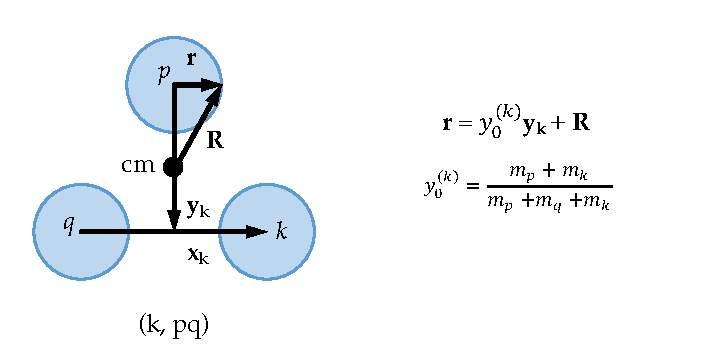
\includegraphics[scale=0.8]{density_scheme_1}
%\decoRule
%\caption{\footnotesize The (k, pq) scheme of Jacobi coordinate %sets for calculation of the density distribution function of %nuclear matter in the framework of  the three body system.}
%\label{fig:density_scheme_1}
%\end{figure}


Write a matrix element of the nucleon operator $\delta \left( {\bf y}_k-y^{(k)}_0 {\bf R} \right)$ via the basis functions:
\begin{align}
&\langle \phi^{JM}_{\gamma i} (k,pq) \vert 
\delta \left( {\bf y}_k-y^{(k)}_0 {\bf R} \right)
\vert \phi^{JM}_{\gamma' j} (k,pq) \rangle = 
 \label{me_delta_k}\\
& =C_i C_j  \int \int d{ x}_k d{ y}_k ~x_k^{2} ~y^{2}_k
~\varphi^{(\lambda,l)}_i(x_k,y_k) 
~\varphi^{(\lambda,l)}_j (x_k,y_k)
\frac{\delta \left( { y}_k-y^{(k)}_0 { R} \right)}{y_k^2} ~
 \delta_{\gamma \gamma'}~ =
 \nonumber \\
&=
C_iC_j  
\left( y_0^{(k)} \right)^{2l}
R^{2l} 
\exp \left( -\tfrac{1}{2} {y_0^{(k)}}^2 \beta^{(k)}_{ij} R^2 \right)
\mathcal{I}\left( 2\lambda+2, \tfrac{1}{2} \alpha_{ij}^{(k)} \right)  \delta_{\gamma \gamma'}.~
\nonumber
 \end{align}
Based on this expression the density function $\rho_k(R)$ of the nucleon $k \equiv N_k$ has form
\begin{align}
\rho^{(N_k)}(R)=&\sum_{\gamma} \rho^{(N_k)}_\gamma(R),
\label{rho_nk}
\end{align}
where
\begin{align}
\rho^{(N_k)}_\gamma(R)=\sum_{ij} 
C_iC_j  
\left( y_0^{(k)} \right)^{2l}
R^{2l} 
&\exp \left( -\tfrac{1}{2} {y_0^{(k)}}^2 \beta^{(k)}_{ij} R^2 \right)
\mathcal{I}\left( 2\lambda+2, \tfrac{1}{2} \alpha_{ij}^{(k)} \right).
\nonumber
\end{align}
If the cluster $k$ is $\alpha$-particle, a relevant matrix element has form
\begin{align}
&\langle \phi^{JM}_{\gamma i} (k,pq) \vert 
\rho_\alpha \left( {\bf y}_k-y^{(k)}_0 {\bf R} \right)
\vert \phi^{JM}_{\gamma' j} (k,pq) \rangle = 
\label{me_rho_alpha}
\\
\nonumber
& = \rho_0 C_i C_j \exp\left(-\gamma_0 R^2 \right)
 \int \int d{ x}_k d{ y}_k ~x_k^{2} ~y^{2}_k
~\varphi^{(\lambda,l)}_i(x_k,y_k) 
~\varphi^{(\lambda,l)}_j (x_k,y_k) \times \\
& \times \exp \left(-\gamma_0 {y_0^{(k)}}^2 y^2_k \right)
i_0(2\gamma_0 y_0^{(k)} y_k R) \delta_{\gamma \gamma'},
\nonumber
\end{align} 
where, $i_0(x)$ is the modified spherical Bessel function of the first kind.
With the aid of this matrix element and using the explicit form of the integral (see. Appendix \ref{AppendixA}), the density function of the $\alpha$-particle $k$ is built as follows
\begin{equation}
\rho^{(\alpha_k)}(R)=\sum_\gamma \rho^{(\alpha_k)}_{\gamma}(R),
\label{rho_alphak}
\end{equation}
where
\begin{align}
\rho^{(\alpha_k)}_\gamma(R)= 
4 \pi \rho_0 \exp\left(-\gamma_0 R^2 \right)
\sum_{ij} C_i C_j 
 \mathcal{I}\left( 2\lambda+2, \tfrac{1}{2} \alpha^{(k)}_{ij}\right) \times \\
 \times \mathcal{I}\left( l,0,\beta_{ij}^{(k)}+2{y^{(k)}_0}^2 \gamma_0,2\gamma_0 y^{(k)}_0 R \right). \nonumber
\end{align}

Let's turn to the density functions of $q$ particles.
 In order to calculate the matrix elements for these particle, one must switch basis functions into $(q,kp)$ Jacobi coordinate set, as in the case with overlap matrix element (\ref{overlap_alternative}). 
In particular, the matrix element for the nucleon $q$ may be represented in the form
\begin{align}
&\langle \phi^{JM}_{\gamma i} (k,pq) \vert 
\delta \left( {\bf y}_q-y^{(q)}_0 {\bf R} \right)
\vert \phi^{JM}_{\gamma' j} (k,pq) \rangle = 
\\
&\sum_{\tilde{\gamma} \tilde{\gamma}'}
A^{\tilde{\lambda}' \tilde{l}' \lambda' l'}_{{\bf Q} }
A^{\tilde{\lambda} \tilde{l} \lambda l}_{{\bf Q} }
\langle \phi^{ J M}_{\tilde{\gamma} i}\left(q,kp \right) \vert 
\delta \left( {\bf y}_q-y^{(q)}_0 {\bf R} \right) \vert
\phi^{ J M}_{\tilde{\gamma}^{\prime} j}\left(q,kp \right) \rangle.
\nonumber
\end{align}
Analogously to the  Eq. (\ref{me_delta_k}) the density function of the nucleon $q$ may be represented as follows
\begin{equation}
\label{rho_nq}
\rho^{(N_q)}(R)=\sum_{\gamma} \rho_\gamma^{(N_q)} (R),
\end{equation}
where the component $\gamma$ is
\begin{align}
&\rho_\gamma^{(N_q)}=
\sum_{\tilde{\gamma}ij} 
{A^{\tilde{\lambda} \tilde{l} \lambda l}_{{\bf Q} }}^2
C_iC_j  
\left( y_0^{(q)} \right)^{2\tilde{l}}
R^{2\tilde{l}} 
\exp \left( -\tfrac{1}{2} {y_0^{(q)}}^2 \beta^{(q)}_{ij} R^2 \right) \times 
\\ \nonumber 
& \times
\mathcal{I}\left( 2\tilde{\lambda}+2, \tfrac{1}{2} {\alpha'}_{ij}^{(q)} \right).
\end{align}
Here, it should be reminded that the rotation matrix ${\bf Q}$ also depends on $ij$ indexes (see. Eq. (\ref{q_rotation_matrix}) and (\ref{overlap_to_q})).
And, the matrix element of the density operator for $\alpha$-cluster $q$ may be introduced in the following expression
\begin{align}
&\langle \phi^{JM}_{\gamma i} (k,pq) \vert 
\rho_\alpha \left( {\bf y}_q-y^{(q)}_0 {\bf R} \right)
\vert \phi^{JM}_{\gamma' j} (k,pq) \rangle = 
\\
&\sum_{\tilde{\gamma} \tilde{\gamma}'}
A^{\tilde{\lambda}' \tilde{l}' \lambda' l'}_{{\bf Q} }
A^{\tilde{\lambda} \tilde{l} \lambda l}_{{\bf Q} }
\langle \phi^{ J M}_{\tilde{\gamma} i}\left(q,kp \right) \vert 
\rho_\alpha \left( {\bf y}_q-y^{(q)}_0 {\bf R} \right) \vert
\phi^{ J M}_{\tilde{\gamma}^{\prime} j}\left(q,kp \right) \rangle.
\nonumber
\end{align}
Following simple derivations one may write the density function of the $\alpha$-cluster of three body system in the scheme ${(q,kp)}$  as
\begin{equation}
\rho^{(\alpha_q)}(R)=\sum_{\gamma}\rho^{(\alpha_q)}_{\gamma}(R),
\label{rho_alpha_q}
\end{equation}
where the function $\rho^{(\alpha_q)}_{\gamma}(R)$ is
\begin{align}
&\rho_\gamma^{(\alpha_q)}(R)=
4 \pi \rho_0 \exp\left(-\gamma_0 R^2 \right)
\sum_{\tilde{\gamma}ij} 
{A^{\tilde{\lambda} \tilde{l} \lambda l}_{{\bf Q} }}^2
  C_i C_j 
 \mathcal{I}\left( 2\tilde{\lambda}+2, \tfrac{1}{2} {\alpha'}^{(q)}_{ij}\right) \times \\
 & \times \mathcal{I}\left( \tilde{l},~0,~\beta_{ij}^{(q)}+2~{y^{(q)}_0}^2 \gamma_0, ~2 \gamma_0 y^{(q)}_0 R \right).
 \nonumber
\end{align}

Density functions for the nucleons $N_p$ and $\alpha$-clusters $\alpha_p$ are obtained in the similar way, as with density functions for the nucleon $N_q$ and $\alpha$-cluster $\alpha_q$.



\section{Root mean square radii}
The above deduced density functions are useful for deriving the root mean square (rms) radii. Moreover, the explicit form of some integrals allows to express the rms radius in a convenient form. This would enable the exact value than the value obtained numerically.

The matter rms radius of in the framework of three body system in this work are defined as follows
\begin{equation}
\langle r^2 \rangle_m = 
\frac{m_k}{m} \langle r^2_k \rangle 
+ \frac{m_p}{m} \langle r^2_p \rangle 
+\frac{m_q}{m} \langle r^2_q \rangle, ~~~m=m_k+m_p+m_q,
\end{equation}
while the charge radius is
\begin{equation}
\langle r^2 \rangle_{ch} = 
\frac{z_k}{z} \langle r^2_k \rangle 
+ \frac{z_p}{z} \langle r^2_p \rangle 
+\frac{z_q}{z} \langle r^2_q \rangle,~~~z=z_k+z_p+z_q,
\end{equation}
where $z$ -- charge of the three body system, the rms radii in general way are determined as follows
\begin{equation}
\langle r^2_i \rangle = 
\int_0^{\infty} dr~ r^{4} \rho^{(i)}(r),~~~i\equiv\{k,~p,~q\}.
\label{rms_general}
\end{equation}

In particular, using the Eq.~(\ref{rho_nk}) the rms radius $\langle r_{N_k} \rangle$ for the nucleon $k\equiv N_k$  is defined as follows
\begin{align}
\langle r_{N_k}^2 \rangle =\sum_{\gamma ij} 
C_iC_j  
\left( y_0^{(k)} \right)^{2l+3}
 \mathcal{I}(2l+4, ~\tfrac{1}{2} {y_0^{(k)}}^2 \beta^{(k)}_{ij})~
\mathcal{I}\left( 2\lambda+2, ~\tfrac{1}{2} \alpha_{ij}^{(k)} \right). 
\end{align}
Explicit form of the integral $\mathcal{I} \left( \lambda, ~\alpha\right)$ is given in the Appendix \ref{AppendixA}.
In the case of the $\alpha$-cluster $q$, by means of the Eq. (\ref{rho_alphak}) its rms radii is calculated as follows
\begin{align}
\langle r_{\alpha_k}^2 \rangle =&4 \pi \rho_0
\sum_{\gamma ij} 
 \mathcal{I}\left( 2\lambda+2,~ \tfrac{1}{2} \alpha^{(k)}_{ij}\right) 
 \times \\
 & \times 
 \mathcal{I}\left(1, ~l,~0,~2\gamma_0,~\beta_{ij}^{(k)}+2{y^{(k)}_0}^2 \gamma_0,~2\gamma_0 y^{(k)}_0\right)
 \nonumber
\end{align}
where the integral depending on six arguments is expressed in Appendix \ref{AppendixA}.

Likewise, the rms radii for the particle $q$  in the three body system may be expressed through the density functions $\rho^{(q)}$ . For instance, putting the Eq. (\ref{rho_nq}) into the Eq. (\ref{rms_general}) we can get the rms radius $\langle r_{N_q}^2 \rangle $ for the nucleon $q$:
\begin{align}
\langle r_{N_q}^2 \rangle  = &
\sum_{\gamma \tilde{\gamma}} \sum_{ij} 
{A^{\tilde{\lambda} \tilde{l} \lambda l}_{{\bf Q} }}^2
C_iC_j  
\left( y_0^{(q)} \right)^{2\tilde{l}+3}
 \mathcal{I}(2\tilde{l}+4, ~\tfrac{1}{2} {y_0^{(q)}}^2 \beta^{(q)}_{ij})~
 \times 
\\ \nonumber 
& \times 
\mathcal{I}\left( 2\tilde{\lambda}+2, \tfrac{1}{2} {\alpha'}_{ij}^{(q)} \right).
\end{align}
Inserting Eq. (\ref{rho_alpha_q}) into Eq. (\ref{rms_general}) we obtain the rms radius $\langle r_{\alpha_q}^2 \rangle$  for the $\alpha$-cluster $q$ the following expression 
\begin{align}
\langle r_{\alpha_q}^2 \rangle=&
4 \pi \rho_0
\sum_{\gamma \tilde{\gamma}} \sum_{ij} 
{A^{\tilde{\lambda} \tilde{l} \lambda l}_{{\bf Q} }}^2
  C_i C_j 
 \mathcal{I}\left( 2\tilde{\lambda}+2, \tfrac{1}{2} {\alpha'}^{(q)}_{ij}\right) \times \\
 & \times \mathcal{I}\left(1, ~\tilde{l},~0,~2\gamma_0,~\beta_{ij}^{(q)}+2{y^{(q)}_0}^2 \gamma_0,~2\gamma_0 y^{(q)}_0\right)
 \nonumber
\end{align}

As regards for the particles $p$ in the three body system the rms radii $\langle r_q^2 \rangle$ may be extracted in analogous way as in the case with the particles $q$. 

For calculating charge radii one must use the different parametrizations $\rho_0$ and $\gamma_0$. Provided the $\alpha$-particle has Gaussian density distribution, the parameters may be obtained by using the charge rms radius $\langle r^2 \rangle^{1/2}_{ch}=1.67$ \cite{satchler1979folding} in the Eq. (\ref{rho_alpha_parameters}).

\chapter{Theoretical models describing nuclear reactions} % Main chapter title

\label{Chapter2} % For referencing the chapter elsewhere, use \ref{Chapter1} 

%----------------------------------------------------------------------------------------

\section{Description of elastic scattering}
Descriptions of the scattering of two nuclei are considered in this chapter when the interaction between them is a potential $U$ which may depend on the spins of the two nuclei but not on their internal coordinates. Thus, it cannot excite the nuclei internally or cause the transfer between them. It can only change their relative motion and, perhaps, reorient spins to each other or to the orbital motion. In general, $U$ will be complex \cite{satchler1983}. 

In the case of the colliding the  $a$ + $A$  particles without spin the potential $U\left( r \right)$ is central, depending only on the magnitude of the channel coordinate ${\bf r}$.
The corresponding Shr\"{o}dinger equation may be written explicitly
\begin{equation}
\left( E + \frac{\hbar^2}{2 \mu} {\bf \nabla}^2 - U \left( r \right) \right) 
\chi \left( {\bf r} \right) =0 
\label{es_she1}
\end{equation}
where $\mu$ is the reduced mass of the $a$+$A$ system, $E$ is the energy in the centre-of-mass system.
The $\chi \left( {\bf r} \right)$ wave function is known as distorted waves describing elastic scattering. The expression "distorted wave" is meant to denote distortion away from the plane wave form due to the presence   of the distorting potential $U \left( r \right)$ (see Fig. \ref{fig:scattering_scheme}). Asymptotically, it has the form of an incident plane wave plus outgoing (scattered) spherical waves
\begin{equation}
\chi^{(+)} \left( {\bf k}, {\bf r} \right) \rightarrow
e^{i {\bf k} \cdot {\bf r}} + f \left( \theta \right) \frac{1}{{\bf r}}
e^{i k r}, ~~  {\bf r} \rightarrow \infty
\label{es_chi_assymp_with_f}
\end{equation}
where $f \left( \theta \right)$ is the scattering amplitude. The $(+)$ superscript stands for outgoing plane wave, while incoming spherical waves is the time-reverse of the $\chi^{(+)}$
\begin{equation}
\chi^{(-)} \left( {\bf k}, {\bf r} \right) = 
\left( \chi^{(+)} \left(- {\bf k}, {\bf r} \right) \right)^{*}
\end{equation}


\begin{figure}
\centering
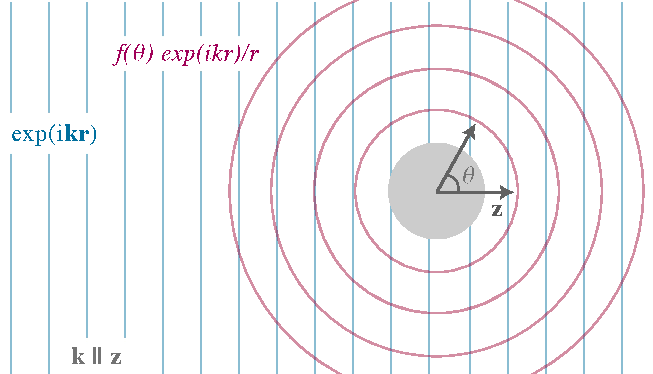
\includegraphics[scale=1]{scattering_scheme}
\decoRule
\caption{ \footnotesize An incoming plane wave scattering off a body making a distorted wave}
\label{fig:scattering_scheme}
\end{figure}

Using the partial wave expansion 
\begin{equation}
\chi^{(+)} \left( {\bf k}, {\bf r} \right) = 
\frac{4 \pi}{kr} \sum_{LM} i^{L} \chi_L \left( k,r \right) 
Y_{LM}\left( \hat{{\bf r}}\right) \left( Y_{LM}( \hat{{\bf k}})\right)^{*},
\end{equation}
A solution for Eq. (\ref{es_she1}) in the absence of any interaction potential, $U \left( r \right) = 0$, is given by 
\begin{equation}
\chi^{(+)} \left( {\bf k}, {\bf r} \right) \rightarrow
e^{i {\bf k} \cdot {\bf r}}, ~~ {\bf r} \rightarrow \infty, 
\end{equation}
for radial part only is written as
\begin{equation}
\chi_L \left( k,r \right)  \rightarrow kr~j_L \left(kr \right),
~~ r \rightarrow \infty,
\end{equation}
where $j_L \left(kr \right)$ is the usual spherical Bessel function. The $\chi_L \left( k,r \right)$ radial function satisfies the radial Shr\"{o}dinger equation
\begin{equation}
\left( \nabla_r + k^2 - \frac{L(L+1)}{r^2} - \frac{2 \mu}{\hbar^2} U \left( r \right)\right) \chi_L \left( k,r \right) =0,
\label{es_she_radial}
\end{equation}
where $k^2 = \frac{2\mu E}{\hbar^2}$.

In the case of the interaction potential has a more sophisticated form, including both Coulomb and nuclear short-range  potentials, the radial Shr\"{o}dinger equation (\ref{es_she_radial}) may be rewritten as
\begin{equation}
\left( \nabla_r + k^2 - \frac{2 \eta k}{r} - \frac{L(L+1)}{r^2} - \frac{2 \mu}{\hbar^2} U \left( r \right) \right) \chi_L \left( k,r \right) =0,
\label{es_she2}
\end{equation}
where $\eta$ is the usual Sommerfeld parameter with the $Z$ charge numbers
\begin{equation*}
\eta=\frac{Z_a Z_A e^2 \mu}{\hbar^2 k}
\end{equation*}
At the radius $r_0$, where the nuclear potential is negligible, Eq.~(\ref{es_she2}) has the solution, which can be expressed in terms of the $\text{H}_L$ outgoing  and $\text{H}_L^*$ incoming Coulomb functions, as follow
\begin{equation}
\chi_L \left( k,r \right) \rightarrow \frac{i}{2}e^{i \sigma_L} \left( \text{H}_L(kr_0)^*
-S_L \text{H}_L(kr_0)\right), 
~~ r \rightarrow r_0
\label{es_assymp_chi}
\end{equation} 
where $\sigma_L$ is the Coulomb phase shift, and it is given with the $\Gamma$ Gamma function as follow
\begin{equation*}
\sigma_L=Arg\left( \Gamma \left( L+1+i \eta \right) \right)
\end{equation*}
In practice, the radial Eq.~(\ref{es_she2}) is solved by numerical integration from $r \approx 0$, then, matched the value and the slope of the result onto the form (\ref{es_assymp_chi}) ar $r=r_0$. This procedure then gives a value for the $S_L$ scattering matrix elements. Having the $S_L$ matrix elements, the amplitude  of the elastic scattering, analogous  from Eq.~(\ref{es_chi_assymp_with_f}), for the $\chi_L \left( k,r \right)$ wave function in the Eq.~(\ref{es_she2}) is given by
\begin{equation}
f(\theta)=\frac{1}{2ik} \sum_{L} (2L+1) e^{2i\sigma_L} \left( S_L - 1 \right)
\text{P}_L(\text{cos}(\theta))
\label{es_amplitude_nuclear}
\end{equation}
where $\text{P}_L(x)$ is the Legendre polynomials, which are solutions to the Legendre differential equation.
By means of the Rutherford scattering amplitude 
\begin{equation}
f_C(\theta)=-\frac{\eta}{2 k {\text{sin}}^2 \left( \tfrac{1}{2} \theta \right) }
e^{\left( i \eta \text{ln}\left( \text{sin}^2 \left( \tfrac{1}{2} \theta \right) \right)
+2i \sigma_{0} \right)}
\end{equation}
the differential cross section of the elastic scattering has the form
\begin{equation}
\frac{\text{d} \sigma_{\alpha}}{\text{d} \Omega} = \vert f_C(\theta) + f(\theta) \vert^2.
\label{es_diff_cross_section}
\end{equation} 
The expression (\ref{es_diff_cross_section}) allows thus to provide comparison with the obtained  experimental data.   


\section{The coupled channels method for inelastic scattering}
The elastic scattering of the projectile $a$ by the nucleus $A$ has been denoted by $\alpha=a+A$. 
 Let $\alpha^{\prime}=a+A^{*}$ be an inelastic channel , in which only the $A$ nucleus has an extra excitation. In the framework of the coupled channel (CC) approach  the total wave function $\Psi$ for the system may be written as
\begin{equation}
\Psi =  \phi_\alpha \left( { x} \right) \chi_\alpha \left( {\bf r}_\alpha \right)+
\phi_{\alpha^{\prime}}  \left( { x} \right) \chi_{\alpha^{\prime}} \left( {\bf r}_{\alpha^{\prime}} \right)
\label{cc_tot_wf}
\end{equation}
 where ${\bf r}$ is the channel coordinate for the partitions $\alpha$ or $\alpha^{\prime}$, $x$ represents the corresponding internal coordinates.
 The total wave function can be part of the Shr\"{o}dinger equation kind of
 \begin{equation}
 H\Psi=E\Psi
 \label{cc_she1}
 \end{equation}
with the Hamiltonian appropriate particular for the $\alpha$ partition
\begin{equation}
H=H_\alpha + K_\alpha + V_\alpha.
\end{equation}
where $H_\alpha \equiv H_a + H_A$ is the internal Hamiltonian for the nuclei $a$ and $A$, $K_\alpha$ is the kinetic energy operator of relative motion and $V_\alpha$ is the interaction potential operator. The wave functions of ground $ \phi_\alpha \left( { x} \right) $ and excited state $ \phi_{\alpha^{\prime}}  \left( { x} \right)$, being eigenfunctions of the internal Hamiltonian $H_\alpha$
 \begin{align}
H_\alpha  \phi_\alpha \left( { x} \right) =& \varepsilon_\alpha \phi_\alpha \left( { x} \right) \nonumber \\
H_\alpha  \phi_{\alpha^{\prime}} \left( { x} \right) =& \varepsilon_{\alpha^{\prime}} \phi_{\alpha^{\prime}} \left( { x} \right),
 \end{align}
have an orthonormality property  of the form 
\begin{equation}
\int {d x} \left( \phi_\alpha \left( { x} \right)  \right)^{*} \phi_{\alpha^{\prime}} \left( { x}\right) =
\delta_{\alpha \alpha^{\prime}}.
\label{cc_orthonorm}
\end{equation}
 Using the expression of total wave function (\ref{cc_tot_wf}), multiplying Eq.~(\ref{cc_she1}) from the left by the $\phi^{*}_\alpha$ function, then, by the $\phi^{*}_{\alpha^{\prime}}$ function, the two coupled equations can be defined in the following form 
 \begin{align}
\left( E -\varepsilon_\alpha - K_\alpha - \langle \alpha \vert V_\alpha \vert \alpha \rangle \right) \chi_\alpha \left( {\bf r} \right) = & \langle \alpha \vert V_{\alpha} \vert \alpha^{\prime} \rangle \chi_{\alpha^{\prime}} \left( {\bf r} \right) 
\nonumber \\
\left( E -\varepsilon_\alpha - K_\alpha - \langle \alpha^{\prime} \vert V_\alpha \vert \alpha^{\prime} \rangle \right) \chi_{\alpha^{\prime}} \left( {\bf r} \right) =&  \langle \alpha^{\prime} \vert V_{\alpha} \vert \alpha \rangle \chi_{\alpha} \left( {\bf r} \right) 
 \end{align}
where $\langle \alpha \vert V_\alpha \vert \alpha \rangle$, or $\langle \alpha^{\prime} \vert V_{\alpha} \vert \alpha \rangle$, is  the matrix element of $V_\alpha$. In particular,  the matrix element $\langle \alpha^{\prime} \vert V_\alpha \vert \alpha \rangle$ is given by
\begin{align}
\langle \alpha^{\prime} \vert V_\alpha \vert \alpha \rangle = & \int d x \phi_\alpha^{\prime} \left( { x} \right)  V_\alpha \left( x,  {\bf r} \right) \phi_\alpha \left( { x} \right) =\nonumber \\
= & V_{\alpha^{\prime} \alpha} \left(  {\bf r} \right).
\end{align}

An expansion of the coupling potential $V_{\alpha^{\prime} \alpha} \left( {\bf r} \right)$ into the $\lambda$ multipoles can be given as follow
\begin{equation}
V_{\alpha^{\prime} \alpha} \left( {\bf r} \right) = \sum_{\lambda \mu} V^{\lambda \mu}_{\alpha^{\prime} \alpha} (r) Y_{\lambda \mu} \left( \hat{r} \right)
\end{equation}

If the potential shape has a deformation, the nuclear potential can be constructed as
\begin{equation}
V_\alpha \left( x, {\bf r}\right) \equiv U\left( r -\delta\left( \hat{r}^{\prime} \right) \right)
\label{cc_coup_pot_def}
\end{equation}
where $\hat{r}^{\prime}$ denotes angular coordinates of $(\theta,~\phi)$ referred to the intrinsic reference frame. The function $\delta\left( \hat{r}^{\prime} \right)$ is normally expanded in multipoles
\begin{equation}
\delta\left( \hat{r}^{\prime} \right) = \sum_{\lambda} \delta_\lambda Y_{\lambda 0} (\hat{r}^{\prime}).
\label{cc_delta_def}
\end{equation}


In the collective model, the ground and excited states are characterized by their angular momenta $I_i$ and $I_{f}$ with projections $M_i$ and $M_{f}$, respectively. For these state the relevant matrix element of the $V_{\alpha \alpha}^{\lambda \mu}$ operator is described using the Wigner-Eckart theorem by
\begin{equation}
\langle I_{i} M_{i} \vert V^{\lambda \mu}_{\alpha^{\prime} \alpha}  \vert I_f M_f \rangle 
= \sqrt{2I_i + 1} 
\langle I_f M_f \lambda \mu \vert I_i M_i\rangle
 \langle I^{\prime} \vert \vert V^{\lambda}_{\alpha^{\prime} \alpha} \vert \vert	 I \rangle.
 \label{cc_we}
\end{equation} 

Using the definitions, (\ref{cc_coup_pot_def}) and (\ref{cc_delta_def}), the reduced matrix element of radial multipoles from Eq.~(\ref{cc_we}) can be rewritten as follow 
 \begin{equation}
 \langle I_{i} \vert \vert V^{\lambda \mu}_{\alpha^{\prime} \alpha}  \vert \vert I_f \rangle = -\frac{\langle I_{i} \vert \vert \delta_\lambda \vert \vert I_f \rangle}{\sqrt{4 \pi}} 
 \frac{\text{d}U(r)}{\text{d}r}
 \end{equation}
 where 
\begin{equation}
\langle I_{i} \vert \vert \delta_\lambda \vert \vert I_f \rangle = \sqrt{2 I_f+1} 
\langle I_f M_f \lambda 0 \vert I_i M_i \rangle 
\langle \chi \vert \delta \vert \chi \rangle \delta_{M_i M_f}.
\end{equation}
The matrix element $\langle \chi \vert \delta \vert \chi \rangle$ is the expectation value of the operator $\delta_\lambda$ in the internal state of the  deformed nucleus. In the framework of the rotational model it can be given with the deformation length $\beta_\lambda$ as follow
\begin{equation}
\langle \chi \vert \delta \vert \chi \rangle = R_0 \beta_\lambda
\end{equation}
where $R_0$ is an average radius of the interaction potential.

The general asymptotic behaviour of the $\chi_{\alpha}$ elastic channel can be taken from Eq.~(\ref{es_chi_assymp_with_f}), while the inelastic channel $\chi_{\alpha^{\prime}}$ may have 
\begin{equation}
\chi_{\alpha^{\prime}} \left( {\bf r}_{\alpha^{\prime}} \right) \rightarrow 
f_{\alpha^{\prime}} \left( \theta \right)
\frac{e^{i k r_{\alpha^{\prime}}}}{r}, 
~~ {\bf r}_{\alpha^{\prime}} \rightarrow \infty
\end{equation}
Note, that the plane wave expression doesn't not present in this equation - only outgoing wave presents. 
A relevant differential cross section for the inelastic channel is obtained from the coefficient of the outgoing wave as follow
\begin{equation}
\frac{\text{d}\sigma_{\alpha^{\prime}} \left( \theta\right)}{\text{d}\Omega} =
\frac{k_{\alpha^{\prime}}}{k_{\alpha}}
\vert f_{\alpha^{\prime}} \left( \theta \right) \vert^2.
\label{cc_dsigma_domega}
\end{equation}
The wave numbers $k_{\alpha}$ and $k_{\alpha^{\prime}}$ follow from the energy conservation 
\begin{equation}
E=\varepsilon_\alpha + \frac{\hbar^2 k_\alpha}{2 \mu} = 
\varepsilon_{\alpha^{\prime}} + \frac{\hbar^2 k_{\alpha^{\prime}}}{2 \mu}.
\end{equation}

\section{The coupled-reaction-channels method for the transfer reactions}
Consider a model for the $a+A\rightarrow b+B$ nuclear reaction, in which entrance and exit channels are denoted as $\alpha$ and $\beta$ respectively. The $\Psi$ total wave function for this model may be given as
\begin{equation}
\Psi = \chi_{\alpha} \left( {\bf r}_\alpha \right) \phi_\alpha \left( x_\alpha \right) + 
 \chi_{\beta} \left( {\bf r}_\beta \right) \phi_\beta \left( x_\beta \right).
\end{equation}
with a model Hamiltonian $H$ such that $\left( E-H \right) \Psi =0$. From the projections of this equation onto the two channels,
\begin{align}
\langle \chi_\alpha \vert \left( E-H \right) \vert \Psi \rangle = 0 \nonumber \\
\langle \chi_\beta \vert \left( E-H \right) \vert \Psi \rangle = 0
\end{align}
with the two equivalent forms of $H$,
\begin{align}
H= H_\alpha +K_\alpha + V_\alpha \nonumber \\
H= H_\beta +K_\beta + V_\beta
\end{align}
one can get a pair of coupled equations for $\chi_\alpha$ and $\chi_\beta$:
\begin{align}
\left[ ~\left(E-\varepsilon_\alpha \right)  -K_\alpha -
\langle \alpha \vert V_\alpha \vert \alpha \rangle ~\right] 
\chi_\alpha ({\bf r}_\alpha) = 
\langle \alpha \vert H-E \vert  \beta \rangle \chi_\beta \nonumber \\
\left[ ~\left(E-\varepsilon_\beta \right)  -K_\beta -
\langle \beta \vert V_\beta \vert \beta \rangle ~\right] 
\chi_\beta ({\bf r}_\beta) = 
\langle \beta \vert H-E \vert \alpha \rangle \chi_\alpha .
\label{crc_couple_eq1}
\end{align}
These are \textit{the coupled-reaction-channels} (CRC) equations. They are integro-differential equations, as may be seen more explicitly in the form
\begin{align}
\left[ ~\left(E-\varepsilon_\alpha \right)  -K_\alpha -
\langle \alpha \vert V_\alpha \vert \alpha \rangle ~\right] 
\chi_\alpha ({\bf r}_\alpha) = 
\int \text{d} {\bf r}_\beta K_{\alpha \beta} \left( {\bf r}_\alpha, {\bf r}_\beta \right) \chi_\beta \left(  {\bf r}_\beta \right)
 \nonumber \\
\left[ ~\left(E-\varepsilon_\beta \right)  -K_\beta -
\langle \beta \vert V_\beta \vert \beta \rangle ~\right] 
\chi_\beta ({\bf r}_\beta) = 
\int \text{d} {\bf r}_\alpha K_{\beta \alpha} \left( {\bf r}_\beta, {\bf r}_\alpha \right) \chi_\alpha \left(  {\bf r}_\alpha \right)
\end{align}
where the kernels are
\begin{align}
K_{\alpha \beta} \left( {\bf r}_\alpha, {\bf r}_\beta \right) = 
J_{\alpha \beta}
\int \text{d} \zeta_\alpha \phi_\alpha^* \left( x_\alpha \right)
(H-E) \phi_\beta \left( x_\beta \right) \nonumber \\
K_{\beta \alpha} \left( {\bf r}_\beta, {\bf r}_\alpha \right) = 
J_{\beta \alpha}
\int \text{d} \zeta_\beta \phi_\beta^* \left( x_\beta \right)
(H-E) \phi_\alpha \left( x_\alpha \right).
\end{align}
Here the internal coordinates have been transformed from the set $x_\alpha$ to the set $\left( \zeta_\alpha, {\bf r}_\beta \right)$, where the $\zeta_\alpha$ are independent of ${\bf r}_\beta$. Also, $J_{\alpha \beta}$ is the Jacobian of this transformation. Then $J_{\beta \alpha}$ is the Jacobian for the analogous transformation form $x_\beta$ to $\left( \zeta_\beta,{\bf r}_\alpha  \right)$.

Since the off-diagonal matrix elements of $V_\alpha$ are small, they have little effect on the elastic scattering and may be neglected on the right side. 
This implies that the elastic scattering in the entrance $\alpha$ channel is described well by the potential $\langle \alpha \vert V_\alpha \vert \alpha \rangle$, and the potential $\langle \beta \vert V_\beta \vert \beta \rangle$ describes well the elastic scattering in the $\beta$ channel.
%Furthermore, if we have one more channel, it is assumed that all couplings, except the direct coupling to the entrance $\alpha$ channel, can be neglected on the right side of the equation for the $\beta$ channel, so that the potential $\langle \beta \vert V_\beta \vert \beta \rangle$ describes well the elastic scattering in this channel. 
By doing this approximation, Eq.~(\ref{crc_couple_eq1}) may be rewritten as
\begin{align}
\left[ ~\left(E-\varepsilon_\alpha \right)  -K_\alpha -
\langle \alpha \vert V_\alpha \vert \alpha \rangle ~\right] 
\chi_\alpha ({\bf r}_\alpha) \approx & 0
 \nonumber \\
\left[ ~\left(E-\varepsilon_\beta \right)  -K_\beta -
\langle \beta \vert V_\beta \vert \beta \rangle ~\right] 
\chi_\beta ({\bf r}_\beta) \approx &
\langle \beta \vert H-E \vert \alpha \rangle \chi_\alpha
\nonumber \\
\approx &
\langle \beta \vert V_\alpha \vert  \alpha \rangle \chi_\alpha + \langle \beta \vert \alpha \rangle (H_\alpha - E_\alpha) \chi_\alpha 
\nonumber \\
\approx & \langle \beta \vert V_\alpha \vert  \alpha \rangle \chi_\alpha
\label{crc_couple_eq2}
\end{align}
 Here the prior interaction, that is the interaction of the $\alpha$ channel, is used. The non-orthogonal term $\langle \beta \vert \alpha \rangle (H_\alpha - E_\alpha) \chi_\alpha$ vanishes because of the $\chi_\alpha$ is on-shell. The usual Green function techniques may then be used to solve these equations and give \textit{the  distorted wave Born approximation transition} (DWBA) amplitude. A detailed representation of the amplitude will be done in the next section. 
% \begin{align}
 %T_{\beta \alpha}^{DWBA} =& \langle \chi_\beta^{(-)} \phi_\beta  \vert V_\alpha \vert
% \chi_\alpha^{(+)} \phi_\alpha \rangle = \nonumber \\
%= & \int \int \text{d}x_\beta \text{d}{\bf r}_\beta \chi_\beta^{(-)*} \left( {\bf r}_\beta \right)\phi_\beta^{*} \left( x_\beta \right) V_\alpha 
% \chi_\alpha^{(+)} \left( {\bf r}_\alpha \right)\phi_\alpha \left( x_\alpha \right)
% \end{align}
% where $\chi^{(+)}$ and $\chi^{(-)}$ obey the homogeneous equations
% \begin{align}
% \left[ ~\left(E-\varepsilon_\alpha \right)  -K_\alpha -
%\langle \alpha \vert V_\alpha \vert \alpha \rangle ~\right] 
%\chi_\alpha^{(+)} ({\bf r}_\alpha) = & 0 \nonumber \\
% \left[ ~\left(E-\varepsilon_\beta \right)  -K_\beta -
%\langle \beta \vert V_\beta^{\dagger} \vert \beta \rangle ~\right] 
%\chi_\alpha^{(-)} ({\bf r}_\alpha) = & 0 \nonumber
% \end{align}
%The differential cross section for the transfer channel $\beta$ can be deduced in the similar way as in Eq.~(\ref{cc_dsigma_domega})

\section{Distorted Wave Born Approximation}
Let consider the nuclear reaction of transfer $\nu$ particle from a $A$ nucleus into a $B$ nucleus:  
\begin{align}
A+b \rightarrow a + B \nonumber \\
A= a + \nu, ~ B=b+\nu
\end{align}
In the case of weak coupling between intermediate channels, it is reasonable to evaluate the transition amplitude in Born Approximation.

In the rearrangement reactions there are few ways to describe the interaction between the different fragments, one for each partition. 
For example,if we choose to describe the scattering in terms of the nuclei of the entrance partition, the projectile-target interaction will be written as
\begin{equation}
V_{Ab}=V_{\nu b} + U_{ab}.
\end{equation}
Here, $V_{\nu b}$ -- a binding potential of the $\nu$ valence particle with the $b$ core, and it is real potential, $U_{ab}$ -- a complex optical potential describing the scattering state of the $a+b$ system.  
In this representation, known as prior mode, the transition amplitude for the transfer process is given by
 \begin{align}
 T_{prior} =& \langle \chi_\beta^{(-)} \phi_a \phi_B  \vert
  V_{\nu b}+U_{ab}-U_{\alpha} \vert
   \chi_\alpha^{(+)} \phi_A \phi_b \rangle = 
   \nonumber \\
= & \int \int d {\bf r}_\alpha  d {\bf r}_\beta
\chi^{-}_\beta \left( {\bf r}_\beta \right)^* 
I_{\beta \alpha}  \left( \left( {\bf r}_\beta ,  {\bf r}_\alpha \right) \right)
\chi^{+}_\alpha \left( {\bf r}_\alpha \right),
 \end{align}
where ${\bf r}_\alpha$ and ${\bf r}_\beta$ -- the radius vectors, illustrated in Fig.\ref{fig:dwba_scheme}, describing relative distance of the $b+A$ and $a+B$ systems respectively,  $U_\alpha$ -- the optical potential describing elastic scattering of $\alpha$-channel, and $I_{\beta \alpha}$ is the kernel function having form
\begin{equation}
I_{\beta \alpha}  \left( \left( {\bf r}_\beta ,  {\bf r}_\alpha \right) \right) =
\left( \phi_a \phi_B  \vert 
 V_{\nu b}+U_{ab}-U_{\alpha} \vert
 \phi_A \phi_b  \right).
\end{equation}
 
\begin{figure}[tp]
\centering
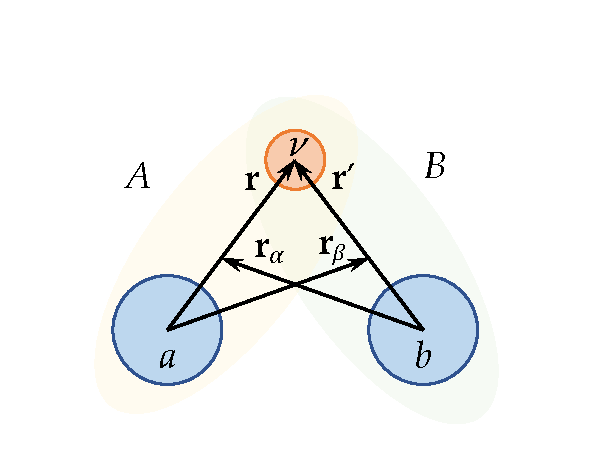
\includegraphics[scale=0.8]{dwba_scheme}
\decoRule
\caption{ \footnotesize The arrangement of radial vectors in the DWBA 
on example of the $A+b \rightarrow a + B$ nuclear reaction. Here $A=a+\nu$ 
and $B=b+\nu$. }
\label{fig:dwba_scheme}
\end{figure} 
 
 Analogously, for the exit channel with $V_{aB}= V_{a \nu}+U_{ab}$ the transition amplitude turns to
\begin{equation}
T_{post}=  \langle \chi_\beta^{(-)} \phi_a \phi_B  \vert
  V_{a \nu}+U_{ab}-U_{\beta} \vert
   \chi_\alpha^{(+)} \phi_A \phi_b \rangle.
\end{equation}
Here, $U_\beta$ stands for the optical potential corresponding to $\beta$ elastic channel. 
 
 The differential cross section for the rearrangement nuclear reaction within the DWBA, in particular for prior form, may be written as
 \begin{equation}
 \frac{d \sigma}{d \Omega}_{DWBA} = \frac{\mu_\beta \mu_\alpha}{2 \pi \hbar^2}
 \left( \frac{k_\beta}{k_\alpha}\right)
 \vert T_{prior} \left( {\bf k}_\beta, {\bf k}_\alpha \right) \vert^2
 \end{equation}
 For the post form the differential cross section is written analogously replacing the corresponding transition amplitude.
 
 In accordance with the DWBA calculations the main ingredients are the internal wave functions for the initial $\left( \phi_A, \phi_b \right)$ and final $\left( \phi_a, \phi_B \right)$ nuclei. 
 In this scheme, the valence particle $\nu$ is bound to the $b$ core to give the composite $B$.
In the simplest picture, the valence particle can be considered a pure single-particle state. 
This means that within this model there is only one possible configuration of the core and valence particle to give the nucleus $B$. Thus, the wave function for the nucleus $B$ can be written as
\begin{equation}
\phi^{JM}_B \left( \xi,~{\bf r} \right) = 
\left[ \phi_b^I (\xi)  \times \phi_{lsj} ({\bf r}) \right]_{JM}
\end{equation}
 In a more sophisticated model, however, the state of the composite contains components of many single particle states coupled to all possible core states.
 Therefore, the wave function $\phi^{JM}_B \left( \xi,~{\bf r} \right) $ may be built as a superposition of the form
 \begin{equation}
 \phi^{JM}_B \left( \xi,~{\bf r} \right)  =
 \frac{1}{\sqrt{n_B}}
 \sum_{Ilj} \mathcal{A}_{lsj}^{IJ} 
 \left[ \phi_b^I (\xi)  \times \phi_{lsj} ({\bf r}) \right]_{JM}
 \label{eq:composite_expansion}
 \end{equation}
 where the coefficients $\mathcal{A}_{lsj}^{IJ} $ are the so called coefficients of fractional parentage or spectroscopic amplitudes. 
 More information about the SA will be introduced in the next section. 
  The squared value of the amplitude is
 \begin{equation}
 S^{IJ}_{lsj} = \vert \mathcal{A}_{lsj}^{IJ}  \vert^2,
 \end{equation}
 which is called spectroscopic factors. 
 The spectroscopic factors can be regarded as the probability of finding the valence particle $\nu$ in a single particle state $l, s, j$ coupled to the core with spin $I$.
 The quantity $n_B$ is the number of nucleons or clusters in the composite system. 
 
Note that the kernel function $I_{\beta \alpha}   \left( {\bf r}_\beta ,  {\bf r}_\alpha \right)  $ involve the overlap between the composite and core wave functions. 
Using the Eq.\ref{eq:composite_expansion} the internal variable $\xi$ in the integral can be explicitly performed giving just unity by normalization
\begin{equation}
\left( \phi^{JM}_B \left( \xi,~{\bf r} \right), \phi_b^I ( \xi ) \right)
\equiv 
\int d \xi \phi^{JM}_B \left( \xi,~{\bf r} \right)  \phi_b^I ( \xi ) = 
\frac{1}{\sqrt{n_B}}
 \sum_{Ilj} \mathcal{A}_{lsj}^{IJ}  \phi_{lsj} ({\bf r})
\end{equation}
 
 The bound wave function $ \phi_{lsj} ({\bf r})$ obey the Shr\"{o}dinger equation 
 \begin{equation}
 \left( T + V_{\nu b} ({\bf r}) + \epsilon - E \right) \phi_{lsj} ({\bf r}) = 0
 \end{equation}
 where $\epsilon$ is the binding energy of the valence particle.
 
 
 
\section{Spectroscopic Amplitudes within the Shell Model}
Spectroscopic amplitudes for nuclear reactions can be obtained by calculations within the shell model. However, this approach is limited in calculating the amount of transferred particles. The calculation of matrix elements for the creation operator is suitable only in the case of the one-particle transfers, or at best two particle transfer. In nuclear reactions with the cluster transfer, one should use other theoretical approaches, or achieve certain values by fitting for the best reproduction of the observables \cite{brown2017}.

Observables for the removal or addition of a nucleon from a specific initial state to a
specific final state are related to the matrix elements of the creation and destruction
operators.
The creation operator $a^+_{km}$ is a tensor of rank $j$ since it creates the single-particle state $\vert km \rangle$. Here, $k$ stands for the set of single-particle quantum numbers $nlj$.
 The destruction operator $a_{km}$ is not a tensor of rank $j$, however,
 \begin{equation}
 \tilde{a}_{km}=(-1)^{j+m} \left[ a^+_{k,-m} \right]^+ =
 (-1)^{j+m} a_{k,-m}
 \end{equation}
is a tensor of rank $j$. And its inverse is $ a_{km}=(-1)^{j-m}\tilde{a}_{k,-m}$. 
Corresponding matrix elements of these operators can be written as
\begin{equation}
\langle
 k^{n-1} \omega^{\prime} J^{\prime}
\vert \vert
\tilde{a}_k
 \vert \vert
 k^{n} \omega^{} J^{}
  \rangle 
  = 
  (-1)^{j+J^{\prime}-J}
  \langle
  k^{n} \omega^{} J^{}
\vert \vert
{a}^{+}_k
 \vert \vert
 k^{n-1} \omega^{\prime} J^{\prime}
  \rangle 
  \label{matrix_elements_of_sa}
\end{equation}
where $\omega$ -- the harmonic oscillator parameter chosen to reproduce the observed mean-square charge radius, $J$ -- total spin of the $n$-particle state.
All many-body matrix elements of $a^+$ can be reduced to these involving a single
$k$-state.

Wave-function expansion relations and sum-rules for the states in the $n-1$ particle system can be obtained by operating with the number operator
\begin{equation}
\hat{N}_k=\sum_m {a}^{+}_{km} {a}_{km}
\end{equation}
on the $k^n$ configuration and then inserting a complete set of states with $n-1$ particles
\begin{align}
\hat{N}_k \vert  k^{n} \omega J M   \rangle   
  &=\sum_m {a}^{+}_{km} {a}_{km} \vert  k^{n} \omega  J M \rangle
   =   n \vert  k^{n} \omega^{} J^{}   \rangle =  \nonumber \\
  &=
  \sum_{m\omega' J' M'}  {a}^{+}_{km} 
  \vert k^{n-1} \omega' J' M' \rangle
  \langle k^{n-1} \omega' J' M'  \vert
  {a}_{km} \vert k^{n} \omega J M \rangle.
\end{align}
The matrix element of $a_{k,m}$ can be reduced with the Wigner-Eckhart theorem
\begin{align}
 \langle k^{n-1} \omega' J' M'  \vert
  {a}_{km} \vert k^{n} \omega J M \rangle = &
  (-1)^{j-m+J'-M'} 
  \begin{pmatrix}
  J' & j & J \\ 
  -M' & -m & M
  \end{pmatrix} \times \nonumber \\
  & \times
  \langle k^{n-1} \omega' J' \vert \vert
  {a}_{km} \vert  \vert k^{n} \omega J  \rangle.
\end{align}
By Eq. \ref{matrix_elements_of_sa} the reduced matrix element of $\tilde{a}$ can be converted in a reduced matrix element of $a^+$ to obtain the final result:
\begin{align}
\hat{N}_k \vert  k^{n} \omega J M   \rangle   &= n \vert  k^{n} \omega J M   \rangle = 
\sum_{m\omega J M} (-1)^{-m-M'+J} 
\begin{pmatrix}
  J' & j & J \\ 
  -M' & -m & M
  \end{pmatrix} \times \nonumber \\
  & \times 
   {a}^{+}_{km} 
  \vert k^{n-1} \omega' J' M' \rangle
  \langle k^{n} \omega' J   \vert \vert
  {a}_{k}^+ 
  \vert \vert
   k^{n-1} \omega' J' M \rangle.
   \label{knmo_basis}
\end{align}
Denoting the $n$-particle wave function by
\begin{equation}
\vert k^n \omega J M \rangle \equiv Z^+ (k^n \omega J M ) \vert	 \rangle
\end{equation}
where $Z^+$ is the linear combination of $a^+$ operator which create the antisymmetric $n$-particle state,
we can thus expand the $k^n$ wave function in terms of those in the $k^{n-1}$ basis:
\begin{equation}
\vert  k^{n} \omega J M   \rangle = 
(-1)^n \sum_{\omega'J'} 
\frac{\langle k^{n} \omega' J   \vert \vert
  {a}_{k}^+ 
  \vert \vert
   k^{n-1} \omega' J' M \rangle }{n\sqrt{2J+1}}
   \left[ Z^+ (k^{(n-1)} \omega' J') \times a^+_k \right]_{JM} \vert \rangle
\end{equation}
A phase factor $(-1)^{n-1}$ arises from commuting $a^+$ with the $n-1$ particles in the state $k^{n-1}$

A sum rule for the matrix elements of $a^+$ can be obtained by multiplying both sides of Eq. \ref{knmo_basis} by $\langle k^n \omega'' J'' M'' \vert$ to obtain
\begin{align}
n \delta_{JJ''}\delta_{MM''}\delta_{\omega \omega''}  &=
\sum_{m\omega' J' M'} (-1)^{-m-M'+J} 
\begin{pmatrix}
  J' & j & J \\ 
  -M' & -m & M
  \end{pmatrix} 
  \times \nonumber \\
  \times &\langle k^n \omega'' J'' M'' \vert a^+_{km} \vert k^{n-1} \omega' J' M'\rangle
  \langle k^{n} \omega J   \vert \vert
  {a}_{k}^+ 
  \vert \vert
   k^{n-1} \omega' J'  \rangle  = \nonumber \\
   =& \sum_{m\omega' J'M'} 
   \begin{pmatrix}
  J' & j & J \\ 
  -M' & -m & M
  \end{pmatrix}
  \begin{pmatrix}
  J'' & j & J' \\ 
  -M'' & -m & M'
  \end{pmatrix} \times \nonumber \\
  \times & 
  \langle k^n \omega'' J'' \vert \vert a^+_{k} \vert \vert k^{n-1} \omega' J' \rangle
    \langle k^{n} \omega J   \vert \vert
  {a}_{k}^+ 
  \vert \vert
   k^{n-1} \omega' J'  \rangle  = \nonumber \\
   = & 
   \frac{\delta_{JJ''}\delta_{MM''}}{2J+1}
   \sum_{\omega' J'} 
   \langle k^n \omega'' J'' \vert \vert a^+_{k} \vert \vert k^{n-1} \omega' J' \rangle
    \langle k^{n} \omega J   \vert \vert
  {a}_{k}^+ 
  \vert \vert
   k^{n-1} \omega' J'  \rangle.
\end{align} 
Then, one finds the sum-rule:
\begin{equation}
\sum_{\omega' J'}
\langle k^n \omega'' J'' \vert \vert a^+_{k} \vert \vert k^{n-1} \omega' J' \rangle
    \langle k^{n} \omega J   \vert \vert
  {a}_{k}^+ 
  \vert \vert
   k^{n-1} \omega' J'  \rangle
   =
   n(2J+1) \delta_{\omega \omega''} \delta_{JJ''}
\end{equation} 
Thus:
\begin{equation}
\sum_{\omega' J'}
\vert 
\langle k^{n} \omega J   \vert \vert
  {a}_{k}^+ 
  \vert \vert
   k^{n-1} \omega' J'  \rangle
\vert^2
=
\sum_{\omega' J'} 
\vert	
\langle k^{n-1} \omega' J'   \vert \vert
  \tilde{a}_{k} 
  \vert \vert
   k^{n} \omega J  \rangle
\vert	^2
=
n(2J+1)
\end{equation}
The matrix elements in which the sum over final states is normalized to unity are historically called coefficients of fractional parentage \cite{de1963nuclear} (CFP) defined by:
\begin{equation}
\mathcal{A}^{JJ'}_{lsj}=\frac{\langle k^{n} \omega J   \vert \vert
  {a}_{k}^+ 
  \vert \vert
   k^{n-1} \omega' J'  \rangle}{\sqrt{n (2J+1)}}
\end{equation}


The reduced matrix elements of the creation and destruction operators
are used to define the SA associated with nuclear reactions.
They are also the building blocks for the more complicated operators associated with
one-body (such as electromagnetic and $\beta$-decay) and two-body transition amplitudes.

\section{Interaction potentials. The double folding model}

The numerical calculations  of the elastic scattering  can be performed in the framework of the OM with the OM potential given by:

\begin{equation}\label{eqn:OP}
\begin{array}{l}
 U(R)=-V^{V}(R)-iW^{V}(R)+V^{SO}(R)( \mathbf{l} \cdot \sigma )\\
~~~ ~~~~~~~+V^C(R),
\end{array}
\end{equation}
where $V^{V}, W^{V}, V^{SO},$ and $V^C$ are real volume,  imaginary volume, spin-orbit and Coulomb potentials, respectively. The volume potentials of colliding two spherical nuclei may be represented as parametrized function. For example, in practice the Woods-Saxon potential is often used, and it has the form
\begin{align}
V^V\left( r \right) = & V_0^V f_{r_V, a_V} \left( r \right), \nonumber \\
W^V\left( r \right) = & V_0^W f_{r_W, a_W} \left( r \right), \nonumber \\
f_{r_0, a_0} \left( r \right) = &  \frac{1}{1+ \text{exp} \left( \frac{r-r_0}{a_0} \right) },
\end{align}
where $V_0$ is depth of the potential, $r_0$ is  average distance and $a_0$ is  diffusion parameter. 

%The surface and 
The spin-orbit term of the OM potential has standard form
\begin{eqnarray}
%W^D(R) &= -4 a_D W_0^D \frac{d}{dR} f^{R_D,a_D}(R), \\
V^{SO}(r) &= V_0^{SO}\left(\frac{\hbar}{m_\pi c}\right)^2 \frac{1}{r} \frac{d}{dR} f_{R_{SO} a_{SO}}(r).
\end{eqnarray}
The Coulomb term has been taken as the interaction of a point-charge with a uniformly charged sphere
\[
\label{coul}
V^C(r)=
\begin{cases}
\frac{Z_1 Z_2 e^2}{2 r_C} \left( 3- \frac{r^2}{r_C^2} \right), &\text{  for } r \leq r_C, \\
\frac{Z_1 Z_2 e^2}{r}, & \text{ for } r > r_C .
\end{cases}
\]



The situation changes, when the colliding nuclei have sophisticated shape. Assume, that there are nuclear matter distribution of the projectile $\rho_a \left( { r}_a \right) $ and target $\rho_A \left( { r}_a \right)$, depending on internal their own radii. Folding the nucleon-nucleon interaction potential $V_{nn}$ over the density distributions of nuclear matter, in the framework of \textit{the Double folding model} an interaction potential may be constructed as follow 
\begin{align}
V^V\left( r \right) = & N_f V^{DF} \left( r \right) \nonumber \\ 
V^{DF} \left( {\bf r} \right) = & \int \int \text{d} {\bf r}_a\text{d} {\bf r}_A
\rho_a \left( {\bf r}_a \right) V_{nn} \left( r_{aA}\right)  \rho_A \left( {\bf r}_A \right). 
\label{df_potential}
\end{align}
where $r_{aA}=\vert {\bf r} + {\bf r}_A - {\bf r}_a \vert$ (see Fig.~\ref{fig:df_scheme}). The $N_f$ normalization parameter is usually fitted in accordance with the dynamics of nuclear reaction of elastic scattering.

\begin{figure}
\centering
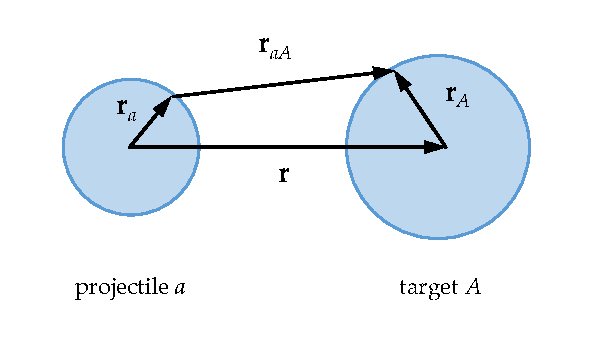
\includegraphics[scale=0.8]{df_scheme}
\decoRule
\caption{ \footnotesize Radius vectors for the double folding model. }
\label{fig:df_scheme}
\end{figure}

The DF potential may be calculated using the effective M3Y-Paris \cite{anantaraman1983effective} nucleon-nucleon potential and the nuclear-matter-densities of projectile and target nuclei. 

 The $V_{nn}$ effective nucleon-nucleon interactions usually are taken as a sum of the three Yukawa potentials, i.e. M3Y-potentials:
 % According to Ref. \cite{anantaraman1983effective, bertsch1977interactions}, for both isoscalar and isovector M3Y-potentials have a form as
 \begin{equation}
 V_{nn}(r)=\sum_{i=1}^{3} N_i \frac{\text{exp}(-\mu_i r)}{\mu_i r}.
 \end{equation}
 
 
The parameters  $N_i$, $\mu_i$ of the M3Y-Paris effective NN-potential \cite{anantaraman1983effective}, often used in the double folding calculations, are given in Tab.\ref{m3y_potpar}.

The dependence $g(E)$ of the folding potential on the collision energy and an additional dependence on the nuclear matter density in the region of their overlap $F(\rho)$ have been phenomenologically established. The folding potential is usually taken as the real part of the optical potential, adjusting its depth to better reproduce the experimental data. The imaginary part of the optical potential is selected in the form of the Woods-Saxon potential, or the same folding potential, while varying its depth.

The potential depending on the collision energy of the projectile, undergoes a change by multiplying a factor
\begin{equation}
g(E)= 1-0.003 \frac{E}{A} .
\end{equation}
An additional dependence of the $V_{nn}$ potential on the total density of colliding nuclei in the region of their overlap may given as
\begin{equation}
F(\rho)=C \left( 1+ \alpha \text{exp} \left( - \beta \rho \right) - \gamma \rho({\bf r})\right).
\label{F_dependence}
\end{equation}
with the parameters
\begin{equation}
C=0.2658 ~~ \alpha=3.8033 \beta=1.4099 ~~ \gamma=4.0
\end{equation} 

 For the particles $t$, $^3$He, $\alpha$, which have simple structure, the density distribution of nuclear matter can be represented as parametrized Gaussian function as follow
 \begin{equation}
 \rho \left( r \right) = \rho _0{\mathrm{exp}}\left( - \alpha_0 r^2 \right)
 \end{equation}
 where the parameters $\rho_0$ and $\alpha_0$ are defined in condition to reproduce the rms matter radii
 \begin{equation}
 \alpha_0 = \frac{3}{2\langle r_{m}^{2} \rangle}, 
 \rho_0 = a  \left( \frac{\alpha_0}{\pi} \right)^{3/2}
 \end{equation}
 here $a$ -- atomic number of projectile. 
 %Для ядер $^3$He величина $\langle r^2_m \rangle^{1/2}= 1.703$ фм \cite{pomerantsev2005dibaryon}.
 
 The density distributions in (\ref{df_potential}) are normalized so that
 \begin{align}
 \int \rho_a ({\bf r}) \text{d} {\bf r}  =a 
 \end{align}
 where $a$ is atomic mass of projectile. For the target nucleus $A$ normalization has the equivalent form.
 
\begin{table}[tp]
\footnotesize
\caption{\label{m3y_potpar} \footnotesize Parameters of the M3Y-Paris \cite{anantaraman1983effective}  NN-potential used in double-folding calculations.}
\begin{tabular*}{\textwidth}{lr@{\extracolsep{\fill}}rrrl}
\toprule
$i$ & $N_i$, MeV &  ~ & ~ & ~ &$\mu_i$, $fm^{-1}$ \\
~& Direct T=0~  & Exchange T=0 & Direct T=1 & Exchange T=1&  \\
 \midrule
1  & 11061.60 & -1524.25  & 313.62 & -4118.9 & 4.0000 	\\
2 & -2537.5  & -518.75 & 223.5 & 1054.75 & 2.5000  \\ 
3 & 0.0  & -7.84 & 0.0 & 2.62 & 0.7072  \\ 
\bottomrule
\end{tabular*}
\end{table}
 
  
As regards target nuclei, having cluster structure, the density distribution of nuclear matter are calculated by means of the three body wave function, and its details are set out in the Section \ref{section_density_function} .

\chapter{The three-body wave functions and their properties}

\section{The three-body wave functions}
\label{section:3bwf}
The three-body wave functions are calculated within the SVM, and obtained parameters for ground state of the $^6$He, $^6$Li and $^9$Be nuclei are listed in Application \ref{AppendixB}. 
The calculations were done using the RSC potential \cite{day1981three} for nucleon-nucleon interaction, 
the SBB potential \cite{sack1954elastic} for  $\alpha$-$N$ interaction and the BFW potential \cite{buck1977local} for $\alpha$-$\alpha$ interaction.  
In Tab. \ref{tab:variational_data} the relative weights of the ground state wave function components and eigenvalues the three body systems are listed\footnote{The obtained data of the variational calculations are not the subject of our research, since the results, perhaps better ones, have already been published and discussed. The purpose of  the section result of the three-body wave function   is to familiarize with what wave function we are dealing with, and its features will be needed in further discussions.}.

Data in Tab. \ref{tab:variational_data} show very good agreement between calculated and measured values of the ground state energy for the \be nucleus.
However, the corresponding values given for the \he and \li nuclei underestimate the experimental data approximately by ~0.5 MeV. 
The discrepancy, probably, due to the non-completeness of the basis function. 
In this work it has no symmetrization, and doesn't enfold an alternative coordinate space.
Other reasons might be in the three-body forces, which has not been included in the variational calculations, and the presence of other cluster components. 
For example, \he can consist of two cluster such as $^3$H + $^3$H, 
the \li nucleus can have $^3$He + $^3$H, and the \be nucleus can be represented as the $^5$He + $^4$He system.
These kind of structures cannot be explicitly included in our model space.
 
% Please add the following required packages to your document preamble:
% \usepackage{booktabs}
\begin{table}[p!]
\caption{ The ground state energies $E_{gs}$ of the three-body systems and the weights of the wave function components found by means of the SVM for the \he, \li and \be nuclei. The set of quantum numbers $\gamma\equiv \lambda l L S$, the dimension $D$ and the probability $P$ of each $\gamma$ are listed. }
\label{tab:variational_data}
\begin{tabular*}{\textwidth}{@{\extracolsep{\fill}}lllllllll@{}}
\toprule
\multicolumn{3}{c}{$^6$He}           & \multicolumn{3}{c}{$^6$Li}           & \multicolumn{3}{c}{$^9$Be}           \\ 
\midrule
\multicolumn{3}{c}{$E_{gs}=-0.228$} & \multicolumn{3}{c}{$E_{gs}=-3.258$} & \multicolumn{3}{c}{$E_{gs}=-1.417$} \\
\multicolumn{3}{c}{$E_{exp}=-0.970$} & \multicolumn{3}{c}{$E_{exp}=-3.70$} & \multicolumn{3}{c}{$E_{exp}=-1.570$} \\
 \midrule
$\gamma$         & $D$       & $P$       & $\gamma$         & $D      $ & $P$       & $\gamma$         & $D$       & $P$       \\
$ \lambda~l~L~S$  &  & & $\lambda~l~L~S$ & && $ \lambda~l~L~S$        &      &      \\
\begin{tabular}[t]{@{}l@{}}0 0 0 0\\ 1 1 1 1\\ 2 2 0 0\\ 3 3 1 1\end{tabular} &
  \begin{tabular}[t]{@{}l@{}}$ 9 \times  9$\\ $ 9 \times  9$\\ $ 5 \times  5$\\ $ 5 \times  5$\end{tabular} &
  \begin{tabular}[t]{@{}l@{}}0.884\\ 0.102\\ 0.010\\ 0.004\end{tabular} &
  \begin{tabular}[t]{@{}l@{}}0 0 0 1\\ 2 0 2 1\\ 1 1 1 0\\ 2 2 0 1\\ 2 2 1 1\end{tabular} &
  \begin{tabular}[t]{@{}l@{}}$ 8 \times 8 $\\ $ 7 \times 7 $\\ $ 7 \times 7 $\\ $ 5 \times 5 $\\ $ 5 \times 5 $\end{tabular} &
  \begin{tabular}[t]{@{}l@{}}0.898\\  0.073\\  0.021\\  0.005\\  0.002\end{tabular} &
  \begin{tabular}[t]{@{}l@{}}0 1 1 1 \\ 2 1 1 1\\ 2 1 2 1 \\ 2 3 1 1 \\ 2 3 2 1 \\ 4 3 1 1 \\ 4 3 2 1\end{tabular} &
  \begin{tabular}[t]{@{}l@{}}$ 7 \times 7 $\\ $ 7 \times 7 $\\ $ 7 \times 7 $\\ $ 6 \times 6 $\\ $ 5 \times 5 $\\ $ 4 \times 4 $\\ $ 4 \times 4 $\end{tabular} &
  \begin{tabular}[t]{@{}l@{}}0.403\\ 0.328\\ 0.235\\ 0.017\\ 0.004\\ 0.009\\ 0.003\end{tabular} \\ \bottomrule
\end{tabular*}
\end{table}
\clearpage



 
\begin{figure}[tp]
\centering
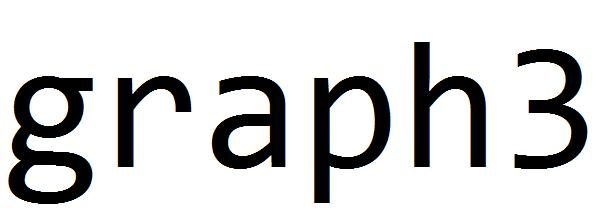
\includegraphics[scale=0.6]{he0_the3D}
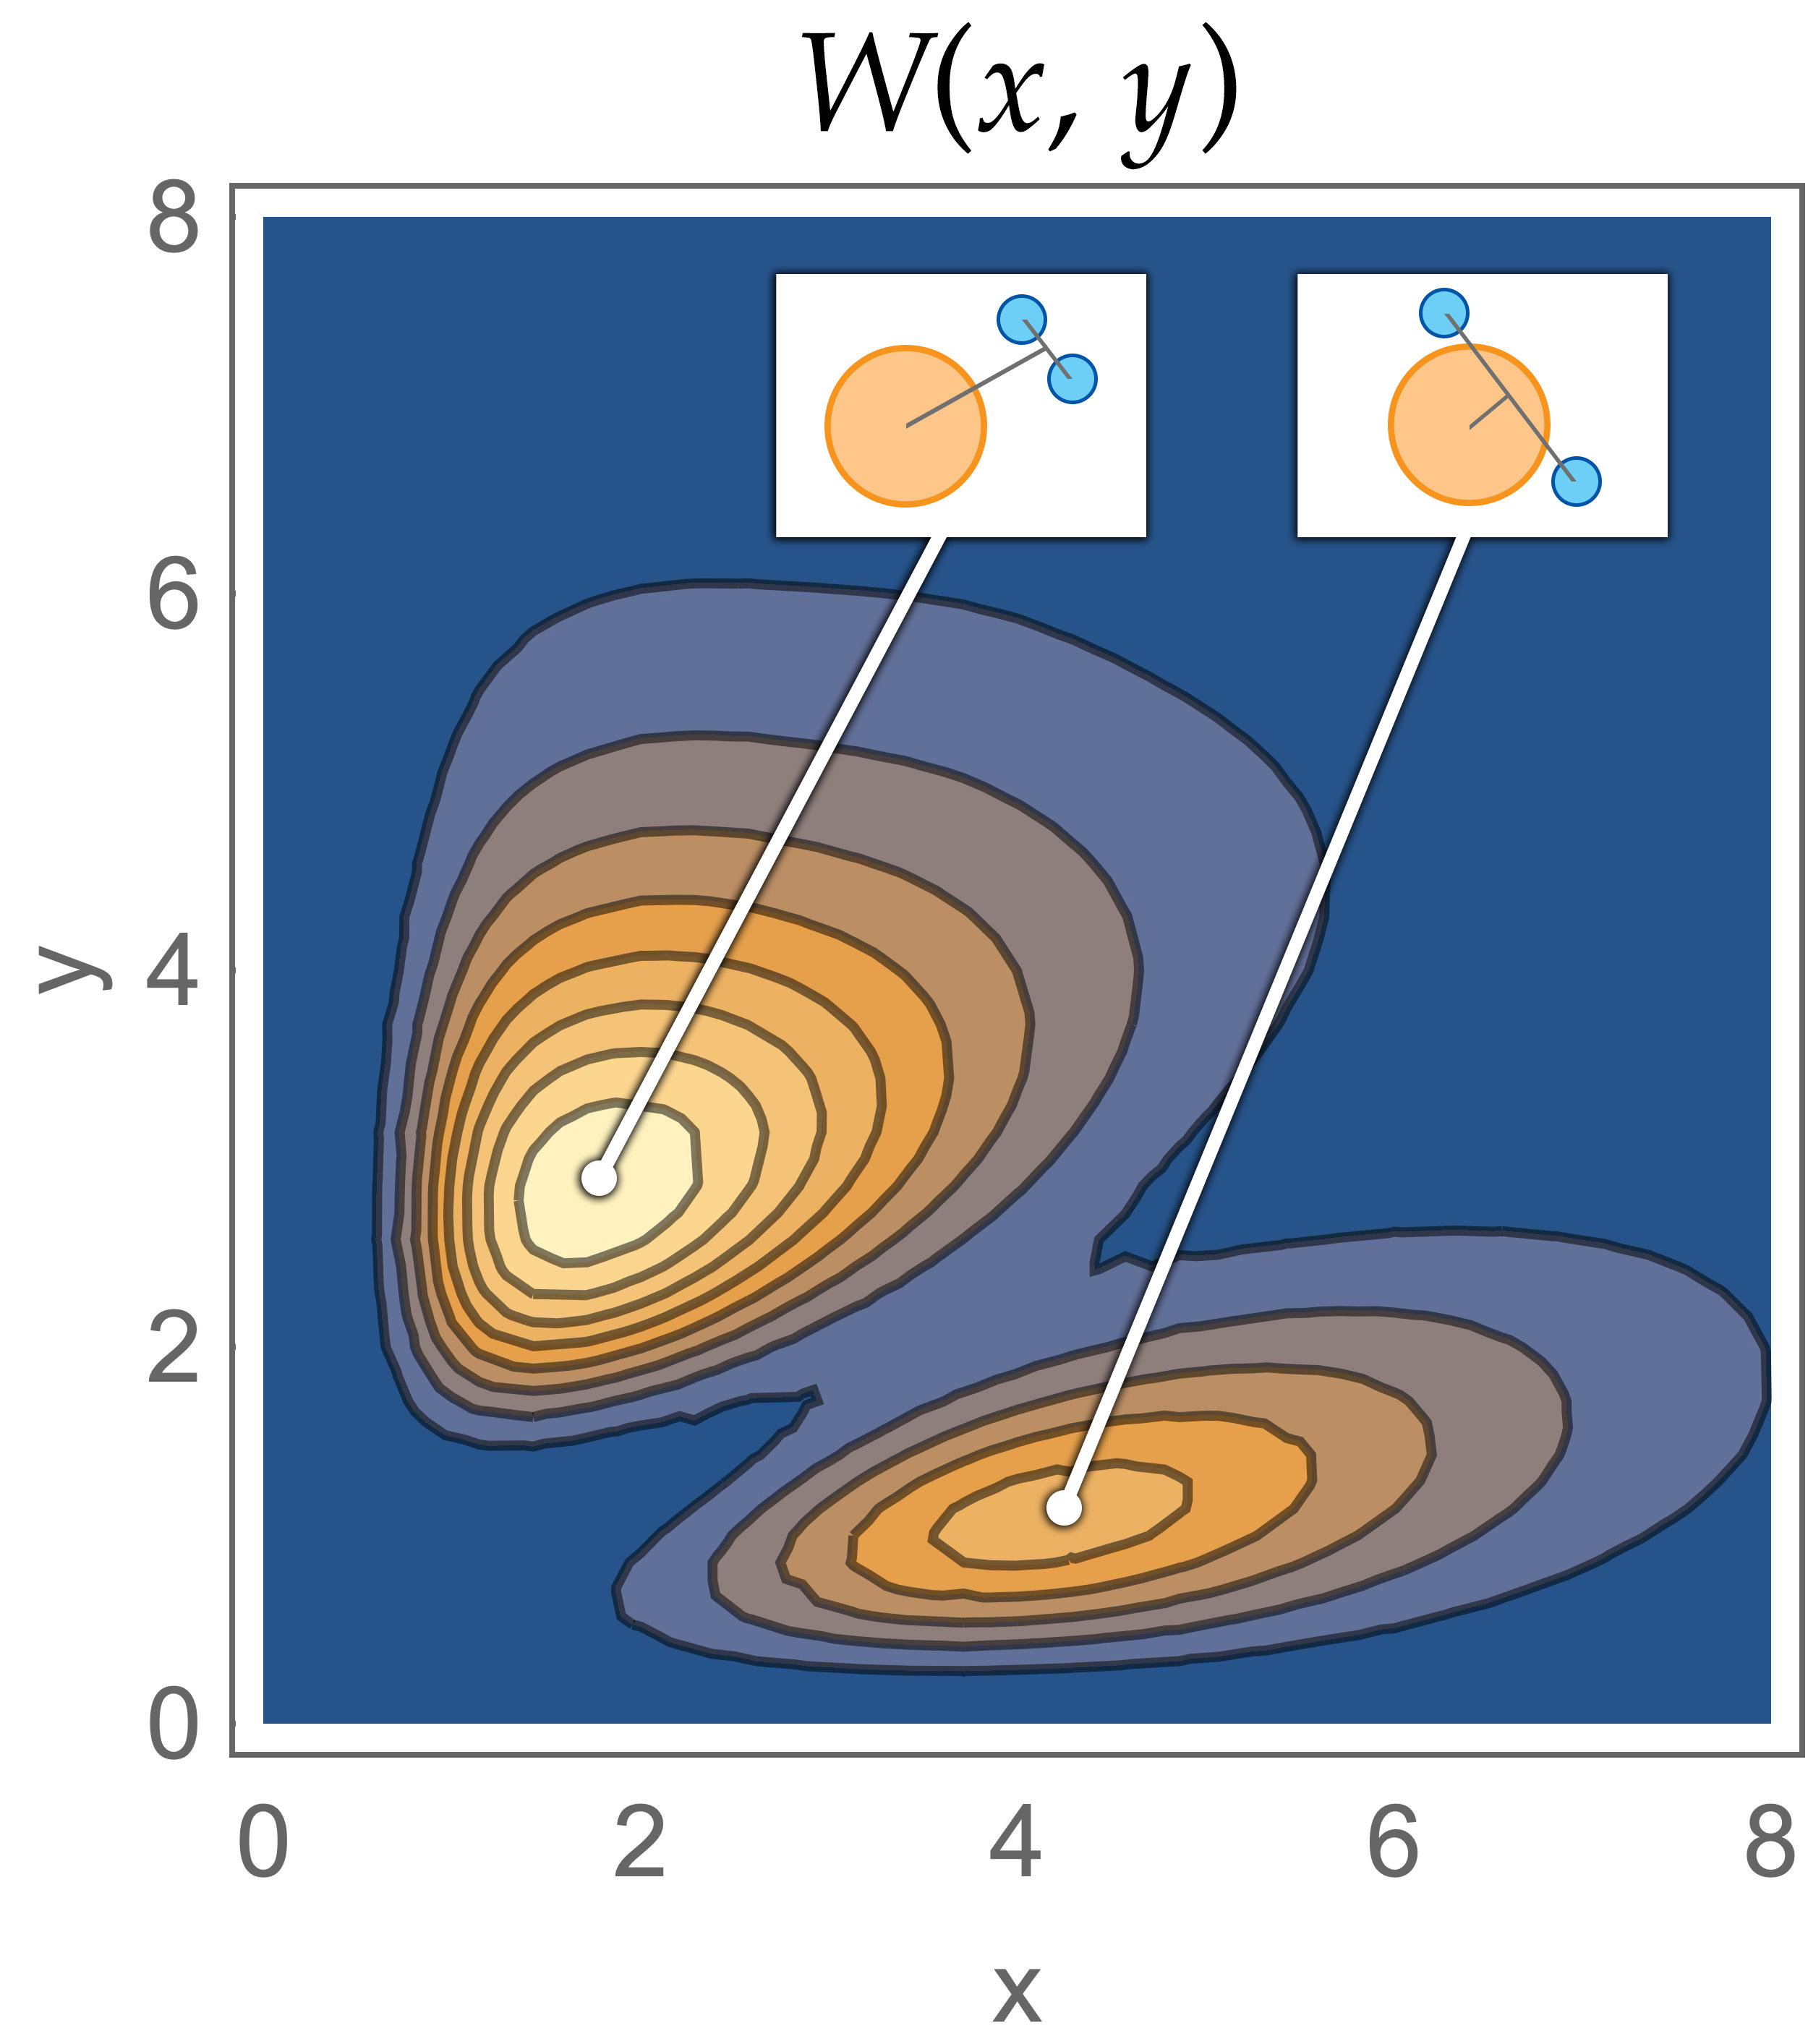
\includegraphics[scale=0.6]{he0_theCP}
\decoRule
\caption{ \footnotesize The correlation function $W(x ,y)$ for the ground state of \he.}
\label{fig:he0_the3D}
\end{figure}


In Figures \ref{fig:he0_the3D}, \ref{fig:li0_the3D} and \ref{fig:be0_the3D} the correlation densities of the three-body wave functions are illustrated in the 3D-Plot form for the $^6$He,  $^6$Li and $^9$Be nuclei. For the purpose of proper visualization the contour-plot are given along. 

\begin{figure}[bp]
\centering
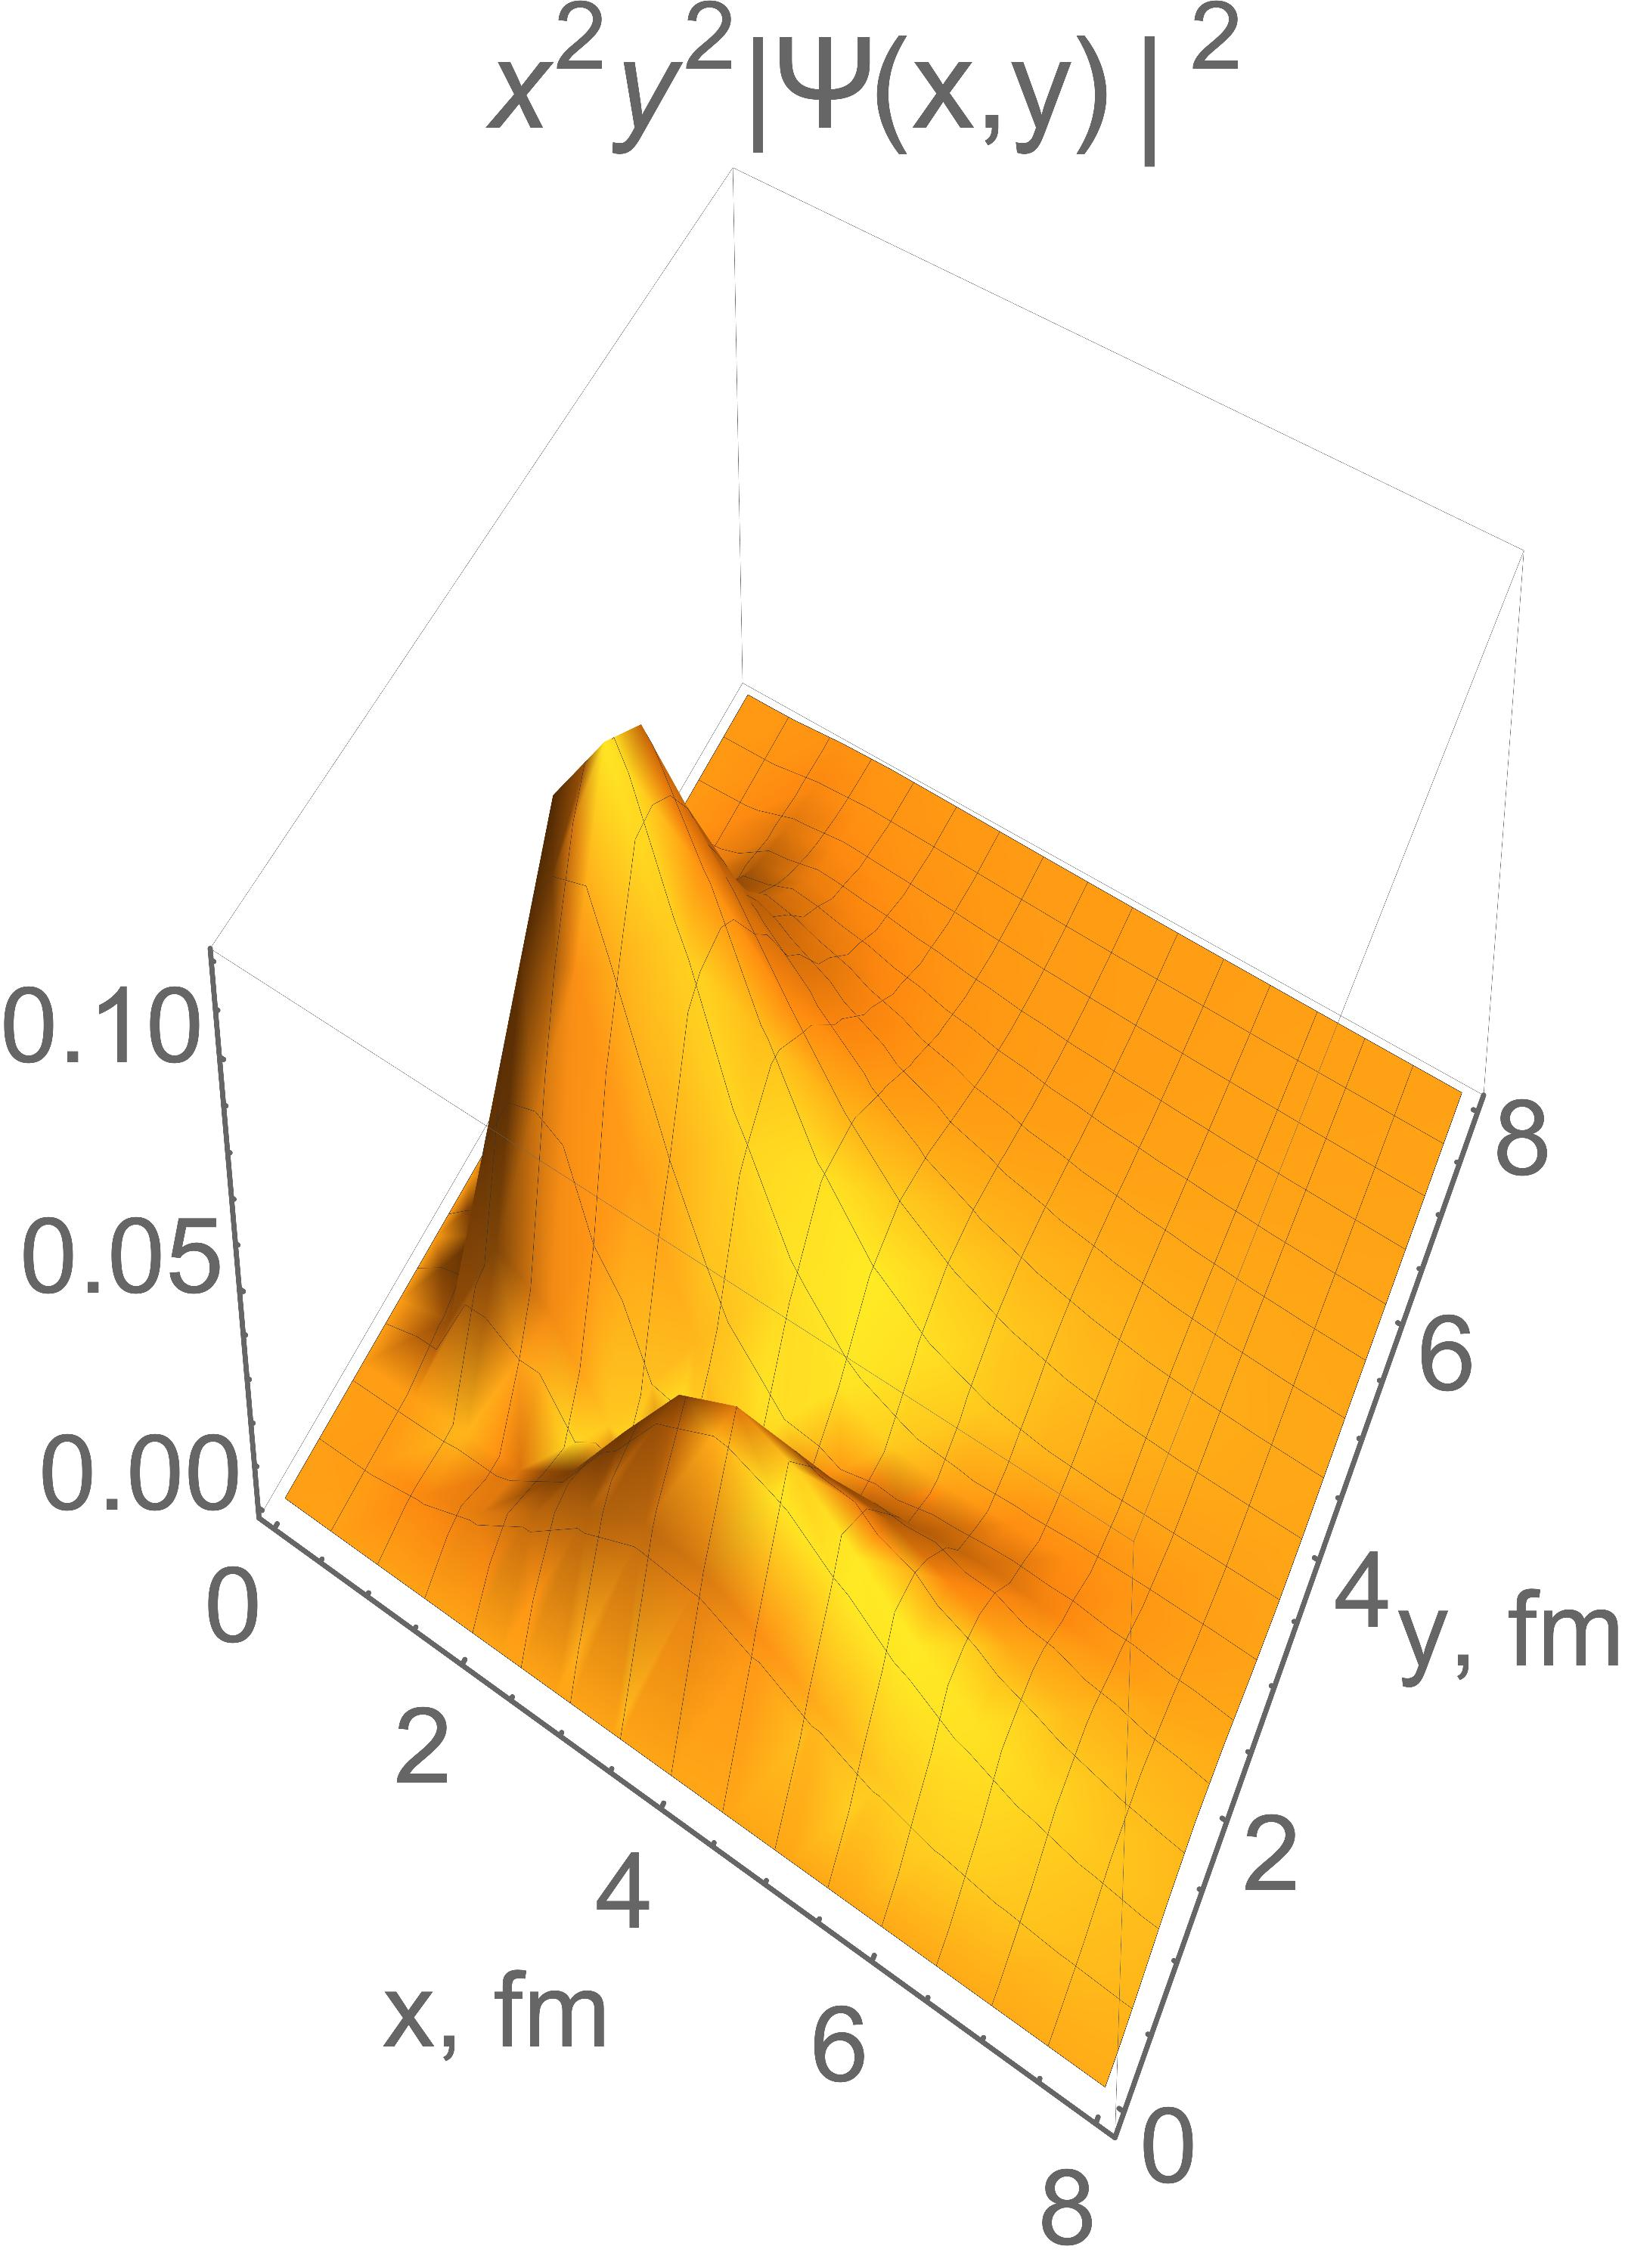
\includegraphics[scale=0.6]{li0_the3D}
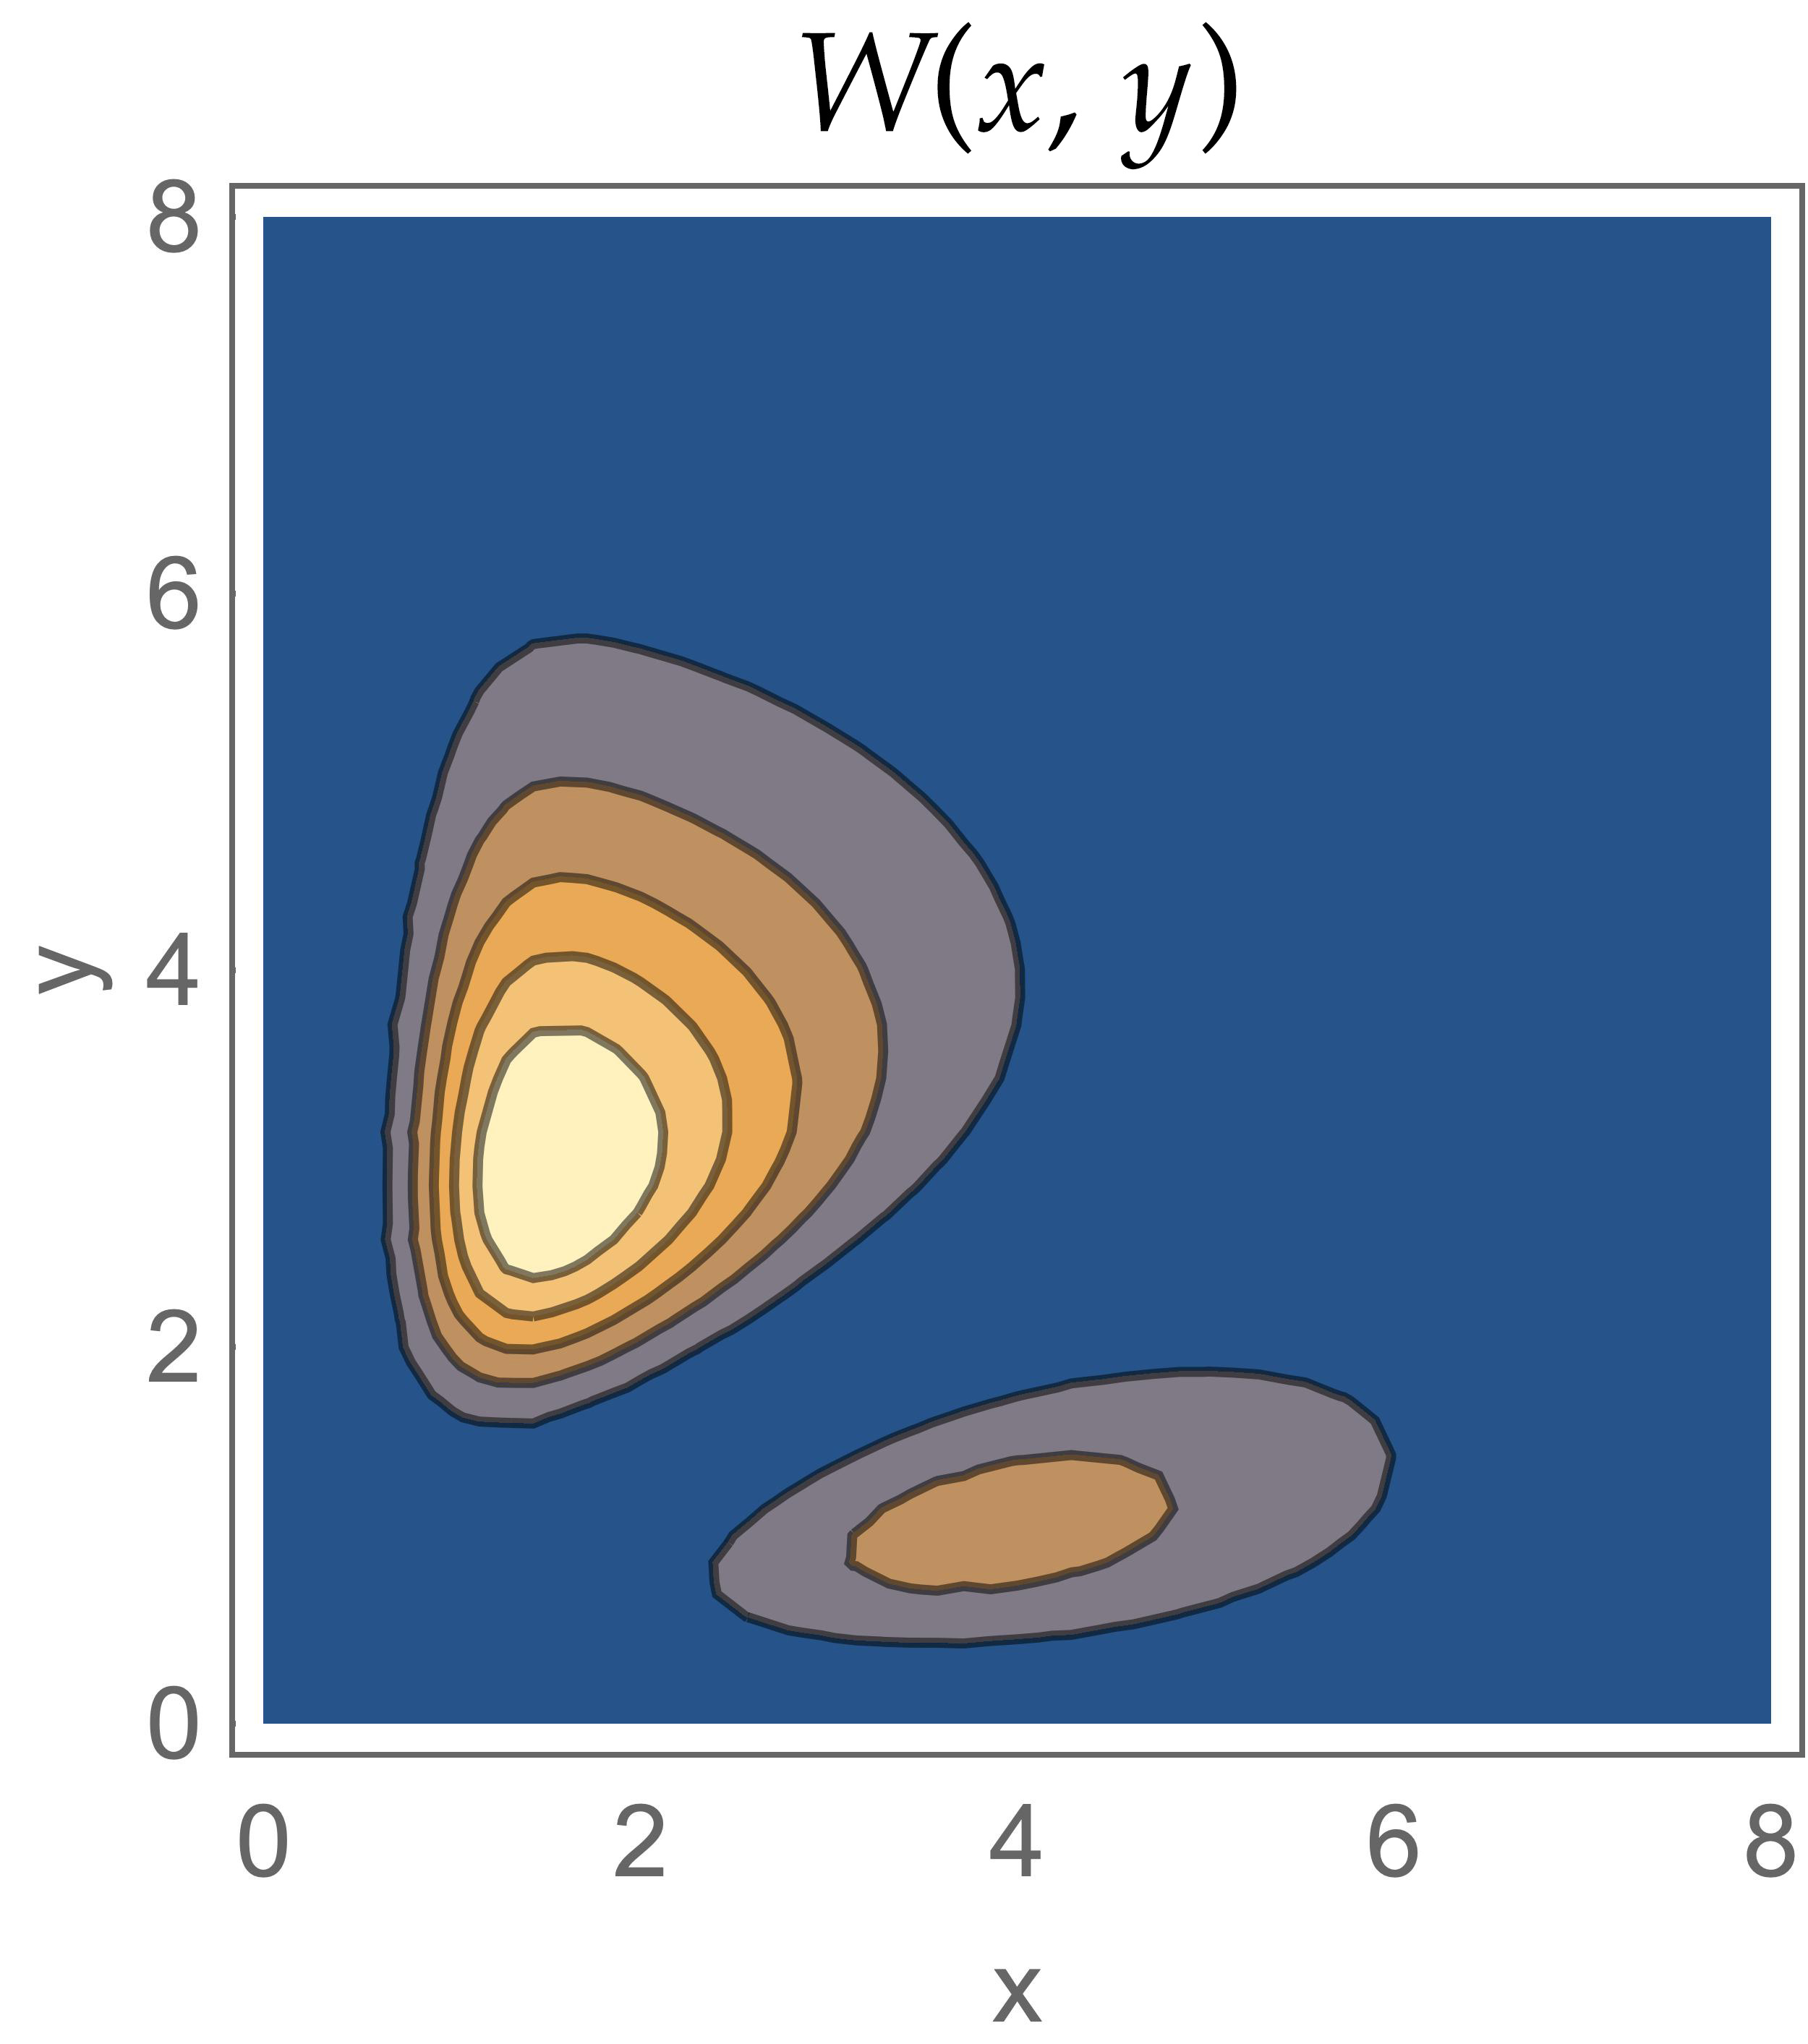
\includegraphics[scale=0.6]{li0_theCP}
\decoRule
\caption{ \footnotesize The same caption as in the Fig.\ref{fig:he0_the3D}, but for \li.}
\label{fig:li0_the3D}
\end{figure} 

In Figures \ref{fig:he0_the3D} and \ref{fig:li0_the3D}, two main geometric configurations can be distinguished, cigar-like component with maximum at the coordinates $(x_k \simeq 4.0~ fm,$ $y_k \simeq 1.0~ fm)$, and di-nucleon component around the coordinates $(1.8~ fm,$ $3.0~ fm)$, both for $^6$He and  $^6$Li nuclei. 
The striking highlight of such geometrical configurations is clear evidence of the cluster structure. 
In particular, we see that in $^6$He, the effect of pairing two nucleons stands out against the background of comparison with $^6$Li. 
Similar results were described in works \cite{kukulin1977stochastic, papadimitriou2011charge}, and were obtained in particularly within the hyperspherical harmonics method \cite{zhukov1993bound}. 

\begin{figure}[tp]
\centering
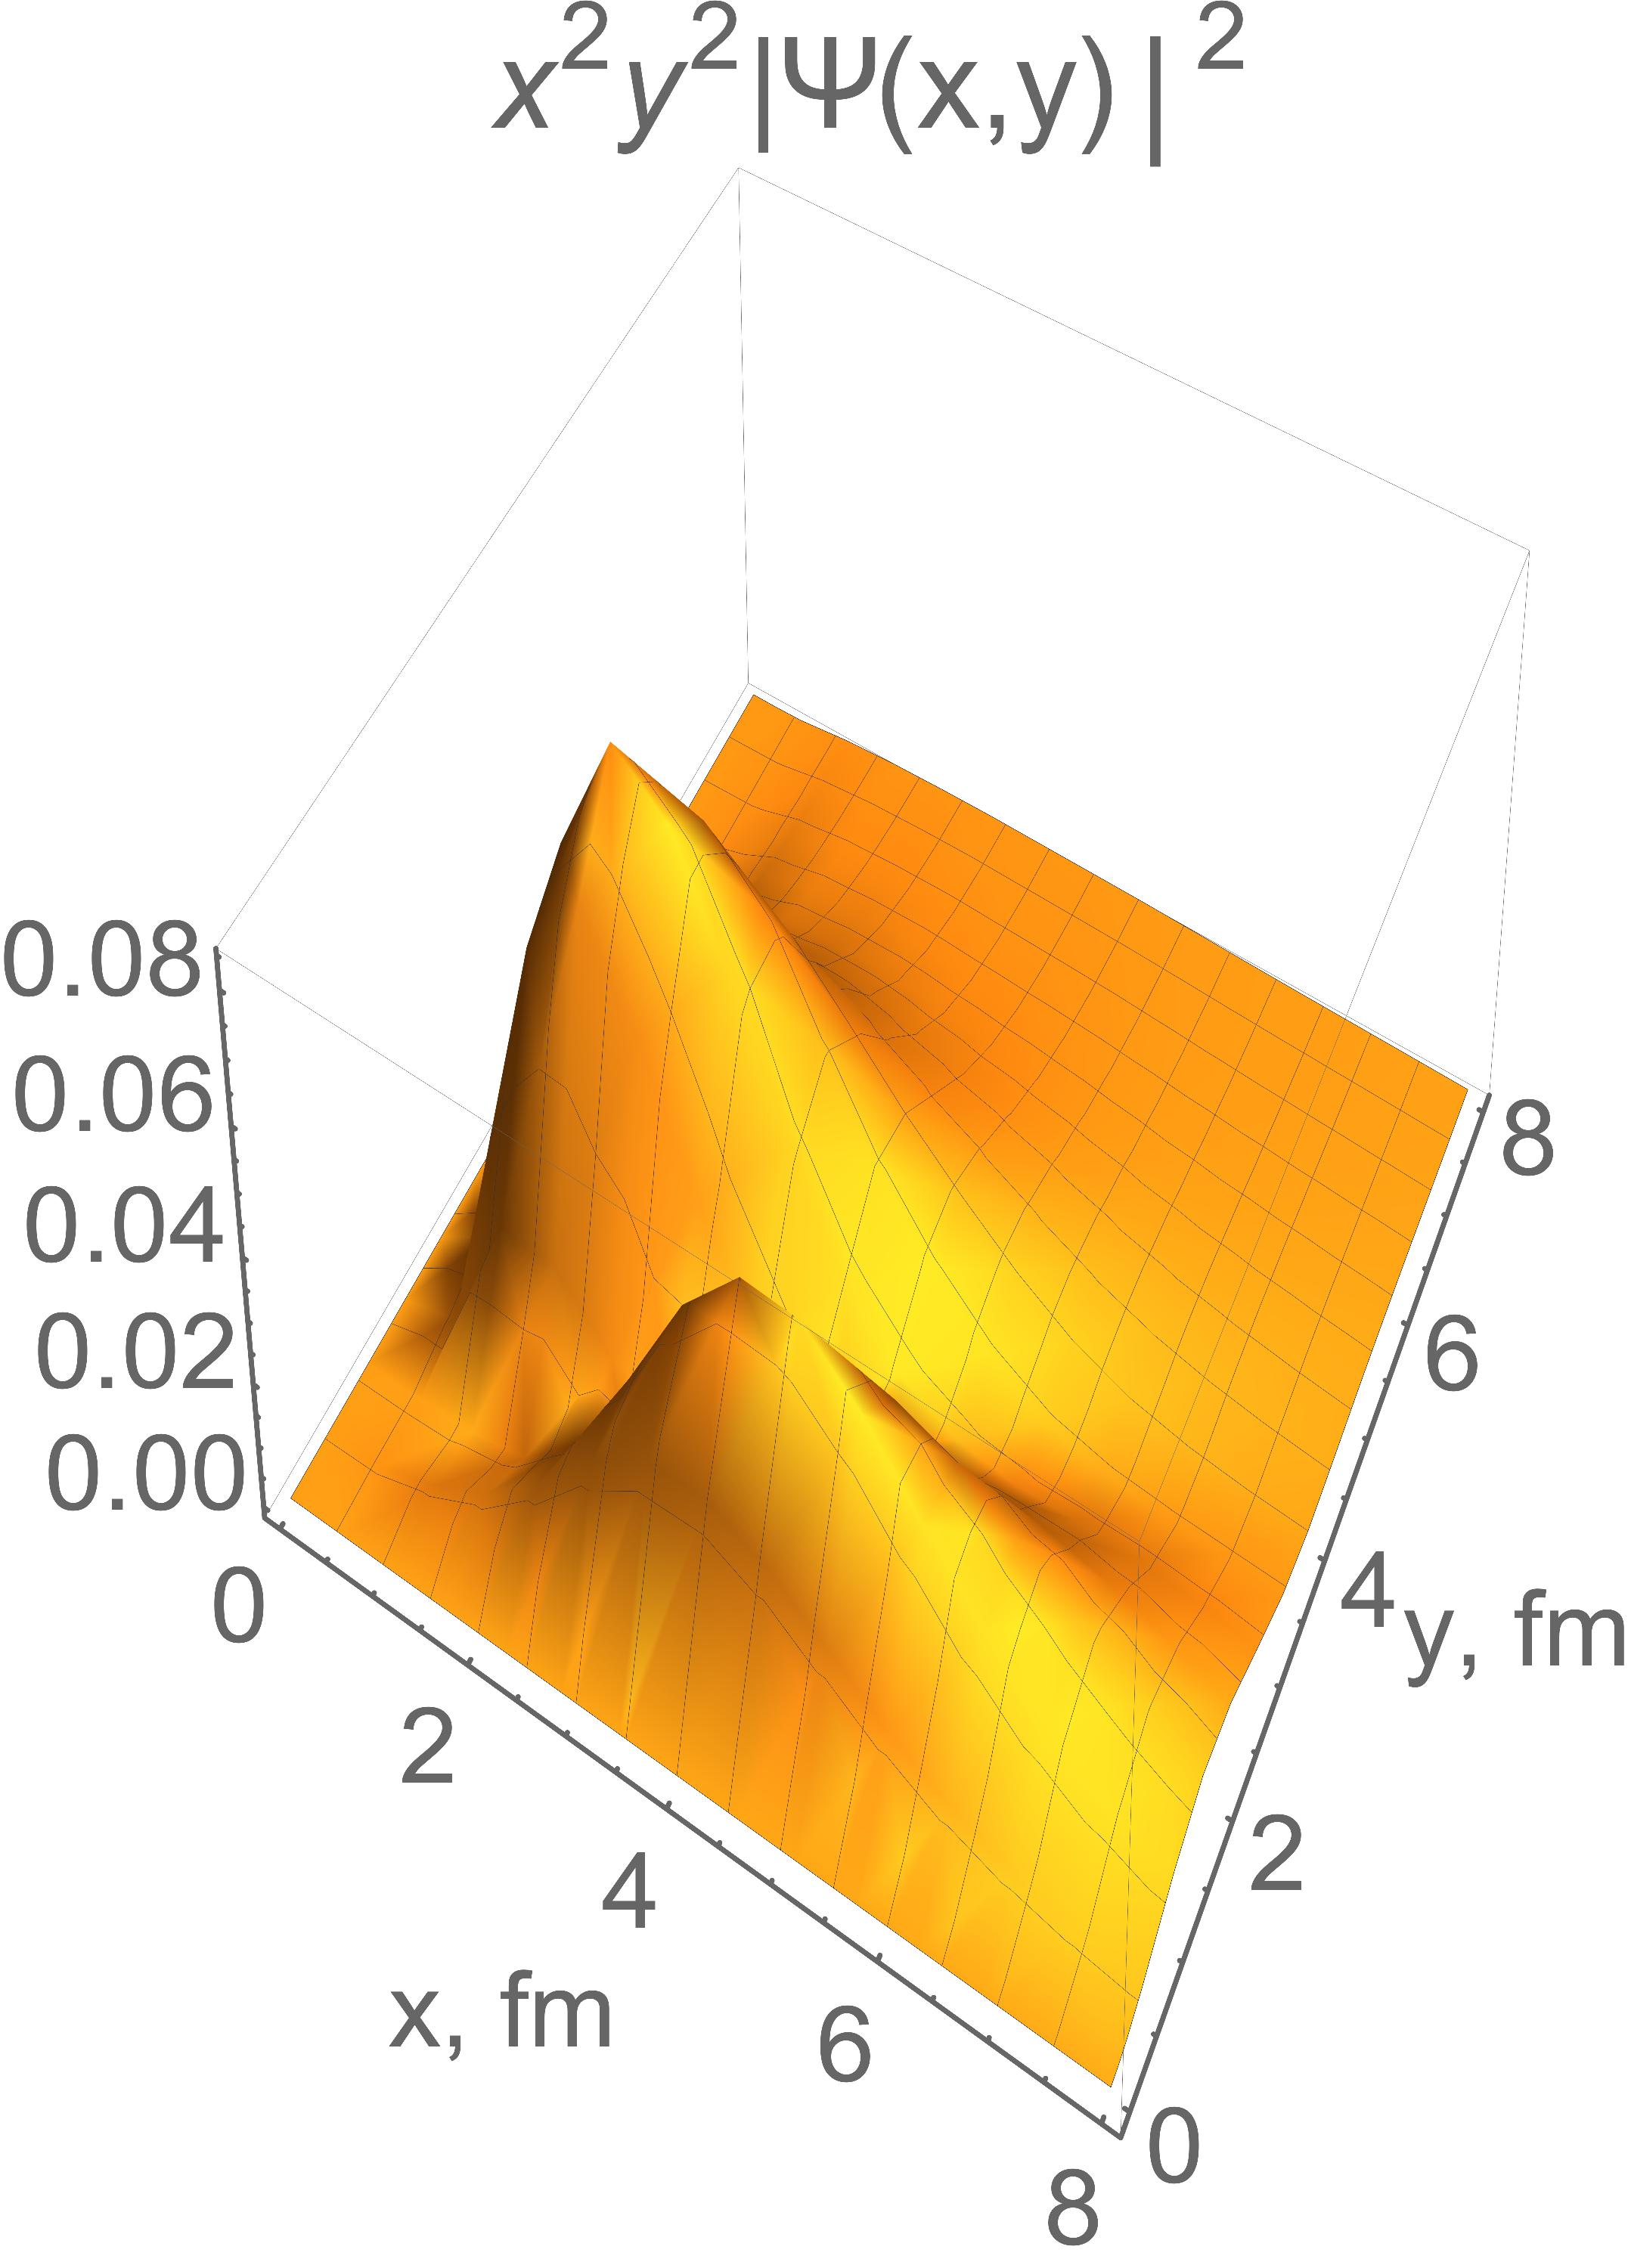
\includegraphics[scale=0.6]{be0_the3D}
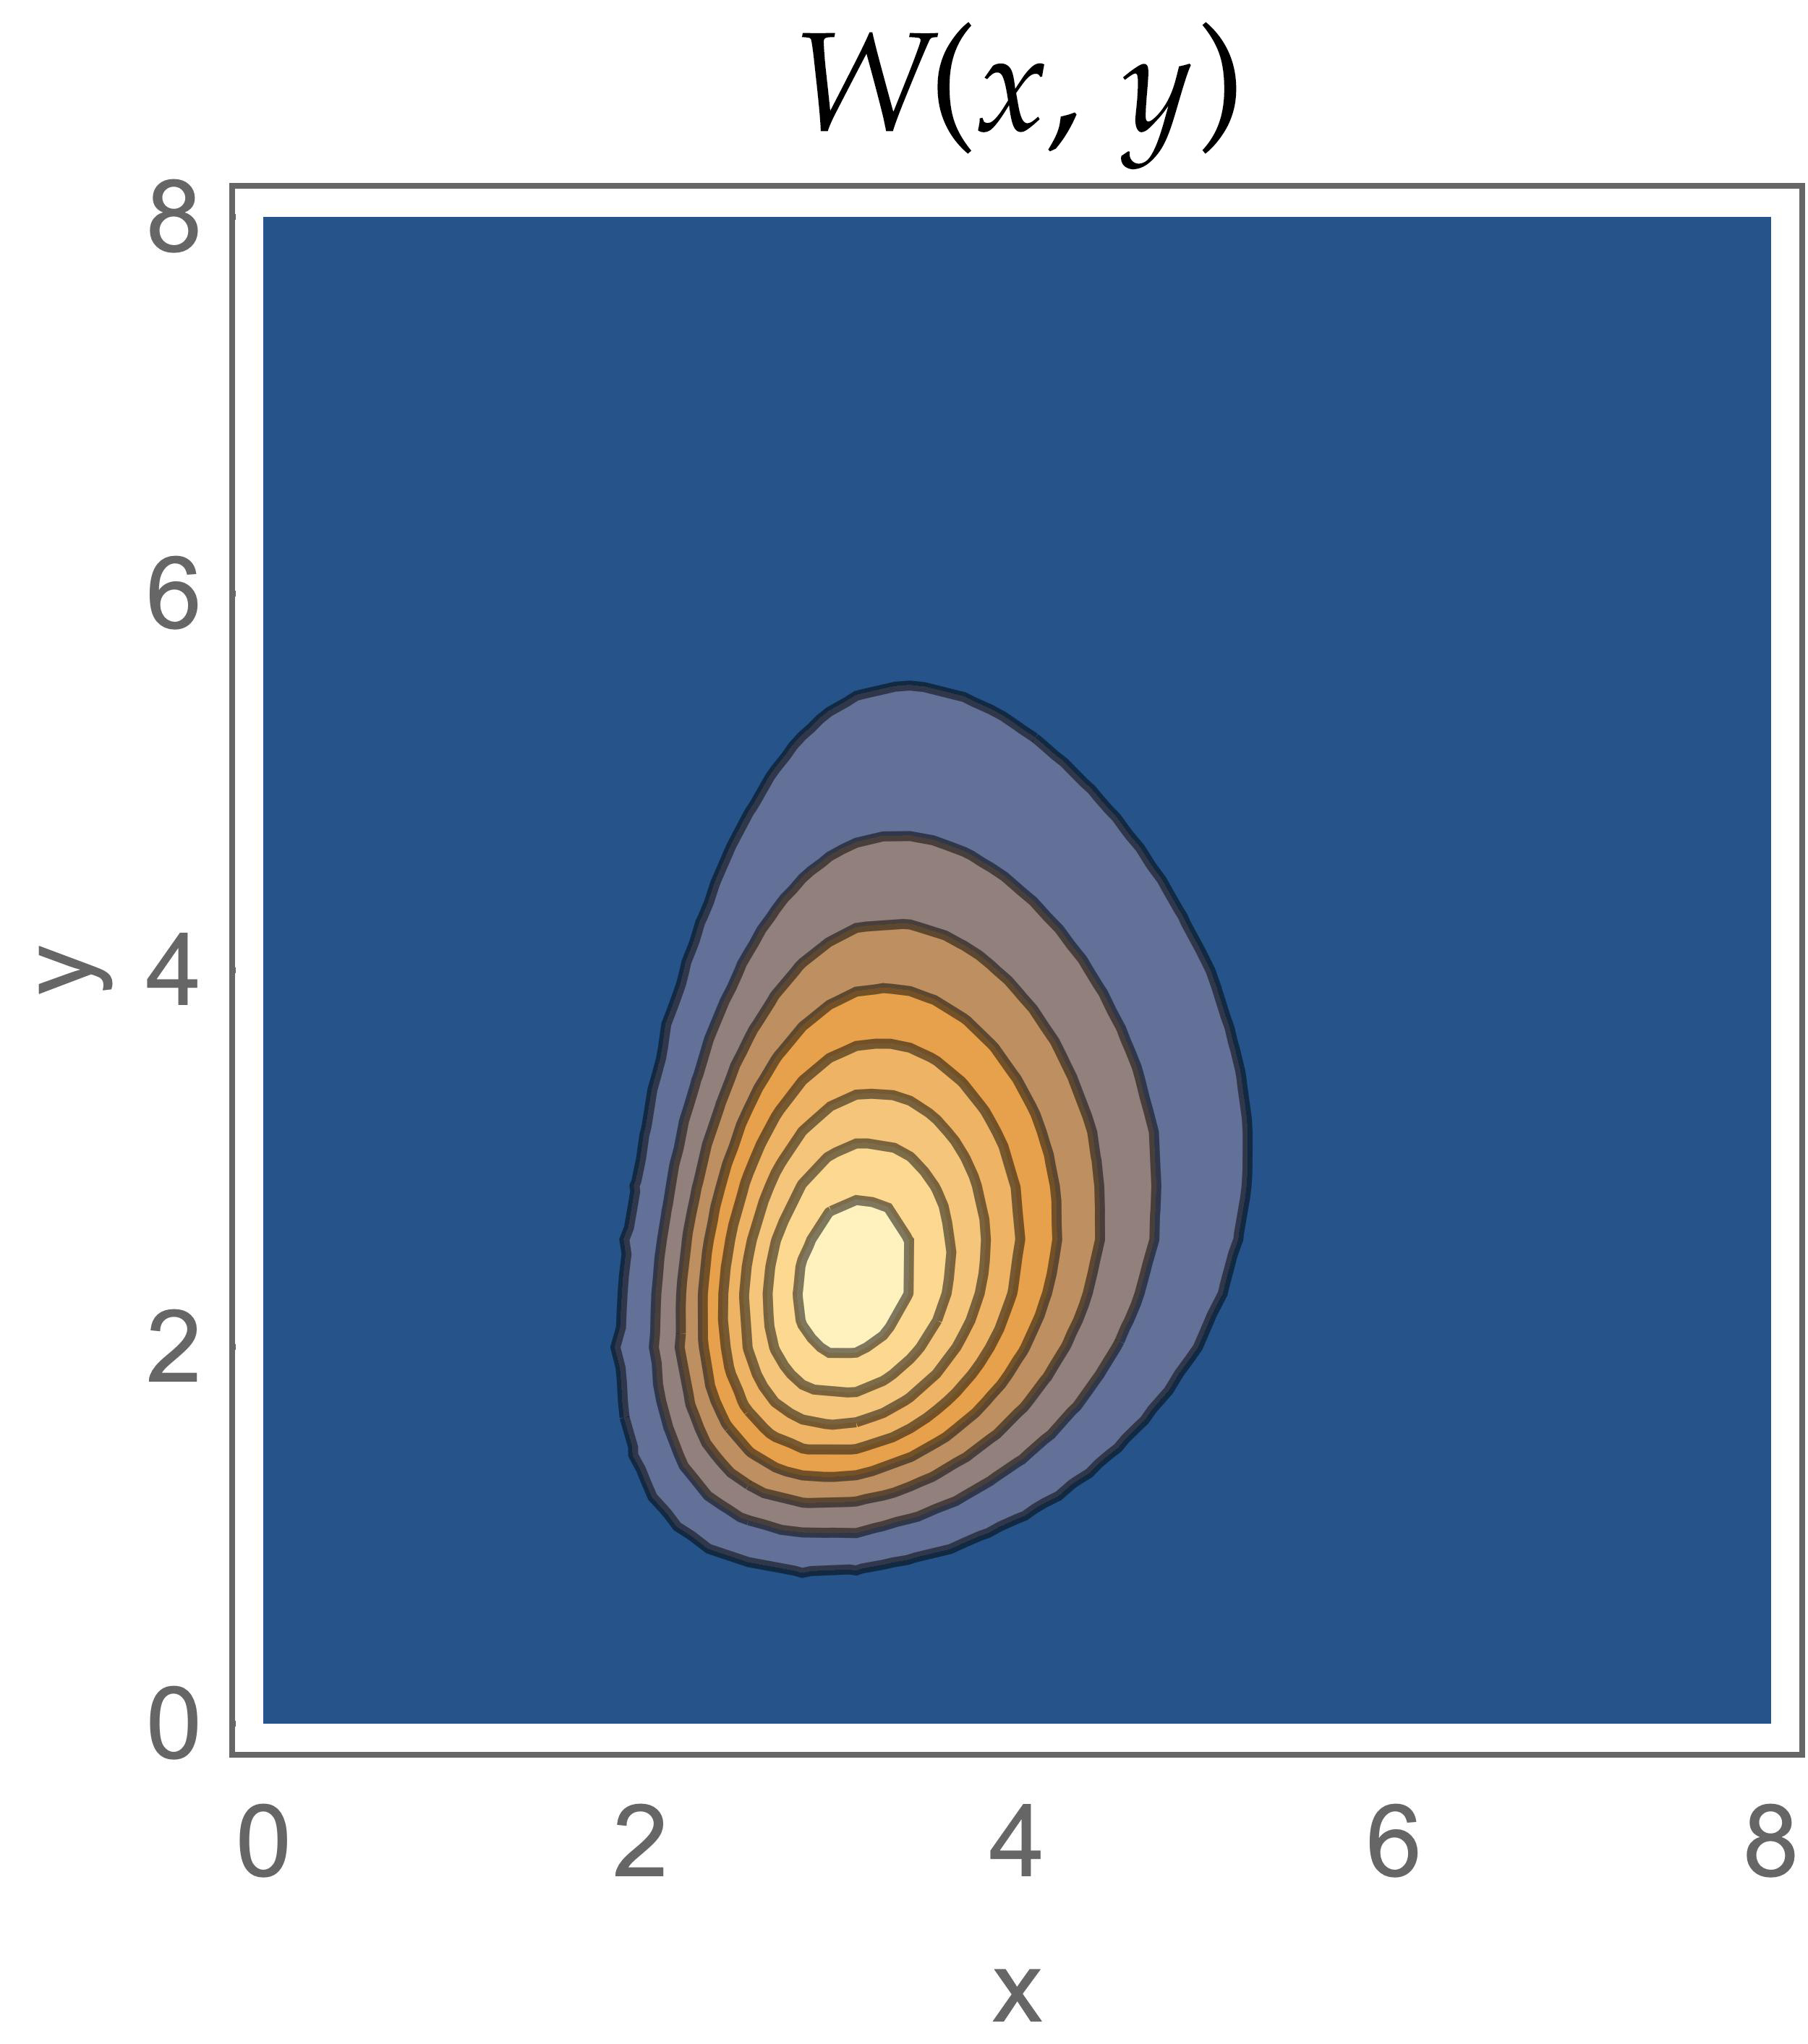
\includegraphics[scale=0.6]{be0_theCP}
\decoRule
\caption{ \footnotesize The same caption as in the Fig.\ref{fig:he0_the3D}, but for \be.}
\label{fig:be0_the3D}
\end{figure} 


The Fig. \ref{fig:be0_the3D} shows the spatial correlation function for the bound state of $^9$Be. 
The single maximum of the correlation density function is located at the coordinates $(x_k \simeq 3.0 ~fm, y_k \simeq 2.0~ fm)$. 
In contrast with the \he and \li nuclei the \be nucleus has only one pronounced spatial configuration corresponding to the two $\alpha$-clusters ($^8$Be ground state) glued by the valence neutron. A very similar picture has been found in Ref. \cite{hussein2015low}. 

\section{Density function of nuclear matter}
On the basis of the three-body wave function in Eq.\ref{totwf}, the nuclear matter density distributions are calculated for $^6$He, $^6$Li and $^9$Be in the ground states using Equations \ref{kpq_density}, \ref{pqk_density_N} and \ref{pqk_density_a}. The results are shown in the Figures \ref{he0_theDD}, \ref{li0_theDD} and \ref{be0_theDD} respectively.
The plotted the density functions are normalized to their own atomic masses. 

\begin{figure}[bp!]
\centering
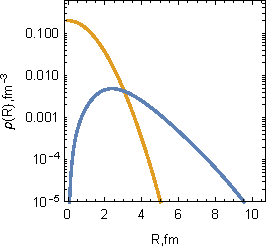
\includegraphics[scale=0.8]{he0_theDD}
~~
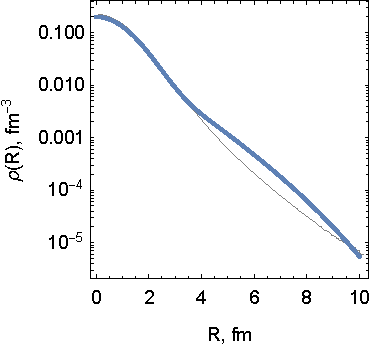
\includegraphics[scale=0.8]{he_density_comp}
 \flushleft 
{\footnotesize ~~~~~~~~$a$)~~~~~~~~~~~~~~~~~~~~~~~~~~~~~~~~~~~~~~~~~~~~ $b$)}
\centering
\decoRule
\caption{  \footnotesize  $a)$: The nuclear matter density distribution of \he with the cluster components contributions; $b)$ Comparison of the total nuclear matter density distribution (blue) of \he with the LSSM calculations (gray dashed)\cite{antonov2005charge}.}
\label{he0_theDD}
\end{figure}


A distinctive feature of the obtained results is in the extended tail of the density function for the \he and \li nuclei in Figures \ref{he0_theDD}.$a)$ and \ref{li0_theDD}. 
This is caused by the properties of the valence nucleons in the three-body system. 
In particular, the density function of the $\alpha$-core $\rho_\alpha^{(k)}(R)$ tends to zero rapidly as the radius $R$ increases. 
The density function of two nucleons $\rho_N^{(p)}(R)+\rho_N^{(q)}(R)$ for \he starts near zero, reaching a maximum near $R \simeq 2.5~fm$, and decreases much more slowly than the density function of the $\alpha$-core.
As regards of \li, it testifies stronger contribution of the deuteron-cluster component in the \li nucleus in comparison with the weight of di-neutron in the \he wave function.
 What is obvious is that the starting value of the  density function $\rho_N^{(p)}(R)+\rho_N^{(q)}(R)$ near zero means that these two nucleons are in the $p$-shell. 
 Thus, we see that the main contribution to the density function starting from $R \simeq 3.0~fm$ is due to two valence nucleons.

A comparison of the total density function $\rho(R)$ for \he with the density function calculated in the framework of the Large-Scale Shell-Model (LSSM), presented in Ref. \cite{antonov2005charge}, is illustrated in Fig.\ref{he0_theDD}.$b)$. Both functions show similar behaviour. However, starting from $R \simeq 4.0~fm$ they becomes different. The density function $\rho(R)$ of \he prevails due to the valence neutron contribution.

\begin{figure}[tp]
\centering
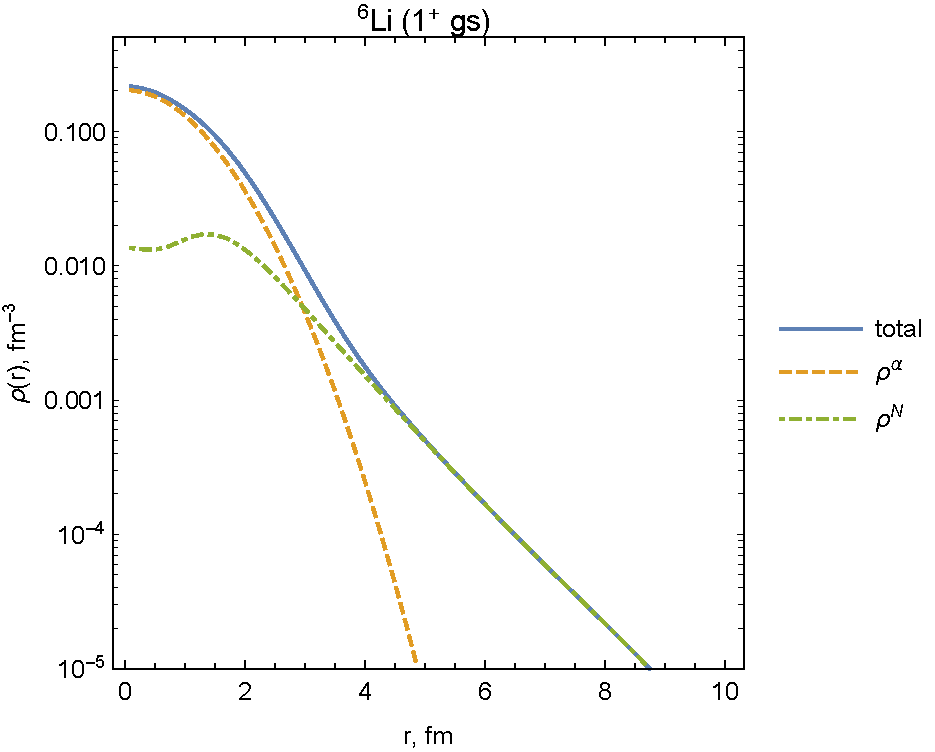
\includegraphics[scale=0.8]{li0_theDD}
\decoRule
\caption{  \footnotesize  The same caption as in Fig. \ref{he0_theDD}, but for $^6$Li. }
\label{li0_theDD}
\end{figure}


\begin{figure}[bp]
\centering
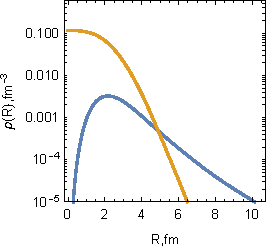
\includegraphics[scale=0.8]{be0_theDD}
\decoRule
\caption{  \footnotesize  The nuclear matter density distribution: contribution of the cluster components are shown. }
\label{be0_theDD}
\end{figure}

The density function $\rho(R)$ of \be has a different shape than the other two previous nuclei (see Fig.\ref{be0_theDD}). The alpha particle density function has become much more voluminous. The nuclear matter density distribution function $\rho_{\alpha}^{(p)}+\rho_{\alpha}^{(q)}$ tends to zero faster than the valence neutron density function $\rho_{N}^{(k)}$ with increasing distance $R$. Starting from the $R \simeq 5.0~fm $ distance, the valence neutron density function $\rho_{N}^{(k)}$  prevails in the nuclear matter contribution. 

The density function of nuclear matter is an excellent subject for studying rms matter radii. With the function $\rho(R)$ we are able to represent the formula for calculating the rms matter radii  $\langle R_{m}^2 \rangle$ as
\begin{equation}
\langle R_{m}^2 \rangle = 
\frac{
\int_0^{\infty} dR~ R^{4} \rho(R)
}{
\int_0^{\infty} dR~ R^{2} \rho(R)
}.
\end{equation}

\begin{table}[bp]
\caption{Comparison the rms matter radii $\langle R_m^2 \rangle^{\frac{1}{2}}$ obtained within the three-body model with other sources.}
\label{tab:rms_matter}
\begin{tabular*}{\textwidth}{@{\extracolsep{\fill}}lccc@{}}
\toprule
 & $^6$He                                                                                                                                                  $(0^+)$ & $^6$Li                                                                                                                                                                                                                                                                                                  $(1^+)$  & $^9$Be                                                                                                                                                                                                                                                                                                  $(\frac{3}{2}^-)$  \\
%  \midrule
$E{gs},$ MeV & --0.228~~--0.970  &--3.258~~--3.700   &--1.417~~--1.570 \\
\midrule
$\langle r^{2}_{ch}\rangle^{1/2},~fm$ & 2.03~~2.00 & 2.63~~2.57   & 2.48~~2.46 \\
$\langle r^{2}_{ch}\rangle^{1/2}_{exp},~fm$ \cite{de1987nuclear}
& ~~~~~~~2.07 & ~~~~~~~2.59   & ~~~~~~~2.52 \\
\midrule
$\langle r^{2}_{m}\rangle^{1/2},~fm$& 2.75~~2.67 & 2.54~~2.49   & 2.58~~2.54 \\
$\langle r^{2}_{m}\rangle^{1/2}_{exp},~fm$ \cite{tanihata1985measurements}
& ~~~~~~~2.75 & ~~~~~~~2.54   & ~~~~~~~2.50 \\
%$\langle r^{2}_m\rangle^{1/2}_{exp}$ , fm \cite{tanihata1985measurements}                                                                                                                                                                              & 2.75  & 2.54 & 2.50 \\

%$\langle r^{2}_m\rangle^{1/2}$ , fm \cite{antonov2005charge}                                                                                                                                                                              & 2.62  & 2.43 & -- \\
%$\langle r^{2}_m\rangle^{1/2}$ , fm \cite{hirai2011clustering}                                                                                                                                                                              & --  & -- & 2.61 \\
  \bottomrule
\end{tabular*}
\end{table}

The calculated results are presented in Tab.\ref{tab:rms_matter}. 
The general picture of the obtained radii shows an overestimation in comparison with other sources \cite{antonov2005charge, hirai2011clustering, tanihata1985measurements}. 
The difference of the calculated matter radii with other lies between $0.15-0.35~fm$. 
It should be noted that the eigen-energies (see Tab. \ref{tab:variational_data}) of the three-body systems does not reproduce the experimental data. 
However, it is noticeable that the greater the difference in the three body eigen-energies with the experimental data, the more the rms matter radii differ.
Therefore, the dependence of the binding energy with the $\langle R_{m}^2 \rangle^{1/2}$ was studied using the example of \he. In order to obtain the binding energy close to the experimental data, the depth of the $\alpha$-$N$ interaction potential, which has a Gaussian shape, was increased from 47 MeV to 49 MeV. Thus, it was possible to reproduce the experimental value of the binding energy of the $2\alpha~+~N$ system. Thus, we managed to get closer those values obtained from other sources.

The reason for the discrepancy between our results and other sources, perhaps, due to the wave function, which is discussed in the previous sections. Nevertheless, knowing the very weak dependence of the density distribution function on the binding energy of the three-body systems, we can use this wave function in calculations to construct interaction potentials within the framework of the folding model.

The obtained Eq.\ref{total_density} also can be used to calculate the rms charge radii. 
Since the wave function is built on the basis of the Gaussian, we can check the correctness of the obtained formulas on the example of rms charge radii if the corresponding parameters of the wave function are available from other sources.
For example, in Ref. \cite{voronchev1994study} the parameters of the three body wave function of the \be ($\tfrac{3}{2}^-$) are listed, and the rms charge radius  is given, $\langle R_{ch}^2 \rangle^{\frac{1}{2}} = 2.34 fm$. 
The calculated rms charge radius by means of our approach pretty agrees with this value. 
The same test has been done for \li, the wave function parameters of which were given by V. Pomerantsev \cite{pomerantsevPrivate}.

In the following calculations the components of three body wave function, contributing less than $10\%$, have been omitted (see Tab.\ref{tab:variational_data}), since the  influence in significantly on the results.

\chapter{Helium-6}
\section{The $\alpha$ + \he nuclear reactions }
\subsection{Elastic scattering}

Calculations of the differential cross section of the elastic scattering for the \he~+~$\alpha$ nuclear reaction has been carried out within the framework of the OM by means of $FRESCO$
\footnote{Further, when it comes to calculations within the framework of the OM, CC and CRC methods, it means that all calculations are performed using the FRESCO code \cite{fresco}.} 
code \cite{fresco}.
The optical potential for the \he~+~$\alpha$ system were calculated with the double folding method using the nuclear matter density of the \he nucleus, discussed in the previous section. 
The potential was built using the three-body wave function of the ground state of \he. 
The folding interactions of $\alpha$-core and two valence nucleon with the $^4$He projectile are presented in Fig. \ref{he_df}.
The calculated double folding potential has structure, reflecting the properties of the \he density distribution.
The potential of the $\alpha$-cluster with the projectile provides the strong central part, while the interaction with hlo neutrons is localized at the peripheral region.

Obtained potential was used to calculate the differential cross section for elastic scattering \he by $\alpha$-particles at energy $ E_{lab} = 151~MeV$. 
The corresponding results are shown in Fig.\ref{he_elastic}. 

In addition to the folding potential, two other potentials (\he-WS1 and \he-WS2) are presented as the Woods-Saxon potential taken from \cite{oganessian1999dynamics}.
 The parameters of the potentials used in the calculations of the theoretical curves within the optical model and the corresponding $ \chi^2 $ are presented in Tab. \ref{tab:he_elastic}.
Theoretical curves are in good agreement with the experimental data at forward scattering angles.
It approves thet the folding potential takes into account all important features of the light exotic \he nuclei.

\begin{figure}[tp]
\centering
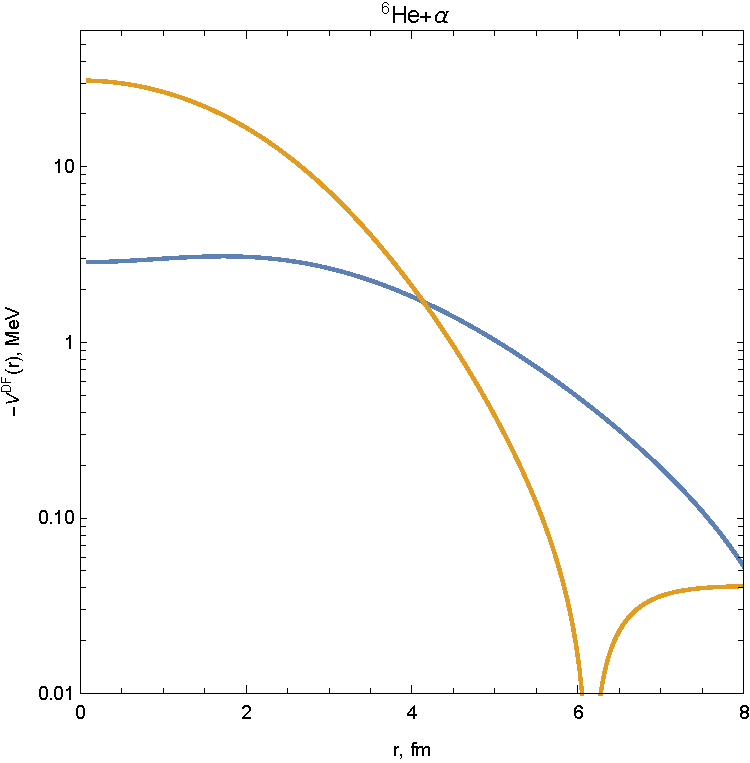
\includegraphics[scale=1]{he_df}
\decoRule
\caption{  \footnotesize  The folding potential $V^{DF}(r)$ in the framework of the three-body model. The potential is for the interaction of the $\alpha$ particle with the constituents of \he.
}
\label{he_df}
\end{figure}

The advantage of folding potential in comparison with others consists of a less number of adjustable optical parameters parameters. Instead of six parameters fitted in the case of Wodds-Saxon potentials, the folding interaction allows to reproduce data fitting only two.



\subsection{Elastic transfer}
In Fig. \ref{he_elastic}.$a)$ theoretical curves were presented to describe the experimental data on elastic scattering. The calculations made within the framework of the optical model showed a good result. However, this is only at the front scattering angles. The backscattering angles are far from the description of optical calculations. Therefore, in order to explain this difference, we propose mechanisms for the transfer of two nucleons: sequential and simultaneous transfer. A schematic representation of the mechanisms can be seen in Fig. \ref{he_transfer_scheme}.  Thus, the differential cross section of these mechanisms can be written as follows
\begin{equation}
\dfrac{d\sigma}{d\Omega}(\theta) =
 \vert f(\theta)_{OM} + f_{sim}(\pi - \theta)+ f_{seq}(\pi - \theta)  \vert^2
\label{eq:he_cs}
\end{equation}


\begin{figure}
\centering
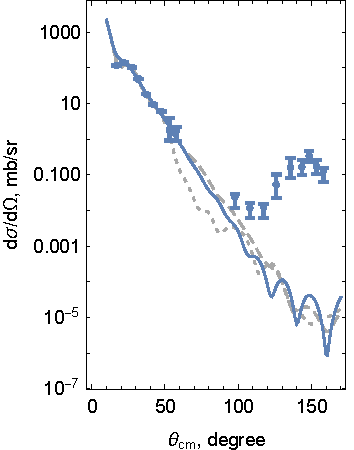
\includegraphics[scale=0.8]{he_elastic}
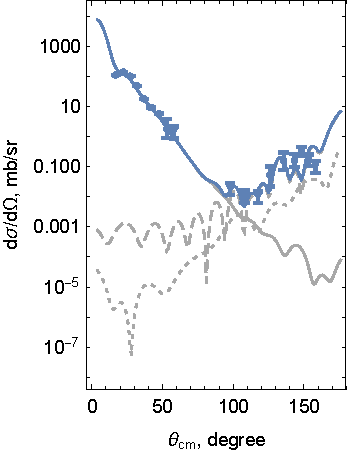
\includegraphics[scale=0.8]{he_elastic_transfer} \\
$~~~~~~a)~~~~~~~~~~~~~~~~~~~~~~~~~~~~~~~b)$
\decoRule
\caption{  \footnotesize  $a)$ The differential cross section of the elastic scattering of \he by $\alpha$-particles at $E_{lab}=151MeV$ calculated with the different potentials: the double folding potential (blue solid), the WS2-\he  (gray dashed) \cite{oganessian1999dynamics} and  WS1-\he (gray dotted) \cite{oganessian1999dynamics}. $b)$ The cross sections of the elastic channel taking into account few possible reaction mechanisms: elastic scattering (solid gray), simultaneous transfer of $2N$ (gray dashed), sequential transfer of $2N$ (dotted) and teit coherent sum (solid blue). Experimental data taken from \cite{oganessian1999dynamics}.
}
\label{he_elastic}
\end{figure}

Calculations for obtaining the differential cross section of the elastic transfer were carried out within the framework of the CRC method. Potential for the input and output channels was taken the double folding potential, and the potential for the intermediate channel was taken the optical potential with global optical parametrizations for $\alpha$ particles \cite{avrigeanu1994global}. Trial calculations have shown that the results depend very little on the selected potential for the intermediate channel.
The results of calculations for elastic transfer made in the framework of CRC are shown in Fig. \ref{he_elastic}.$b)$. 
The sequential transfer of two nucleons is shown by gray dotted curves, their simultaneous transfer by dashed gray curves, the elastic scattering cross section by solid gray curves, and, finally, their coherent sum is shown as a blue solid curve. 
The wave function of the bound states was chosen by fitting the potential depth to the binding energy of the composite systems. 
In particular, the binding energy of one neutron with $^6$He was 1.8 MeV,  neutron with $^5$He -- 0.1 MeV, and two neutrons with  $\alpha$  -- 0.9 MeV. 

\begin{figure}[bp]
\centering
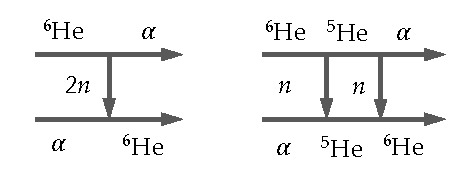
\includegraphics[scale=1]{he_transfer_scheme}
\decoRule
\caption{  \footnotesize  Schematic representation of the elastic transfer nuclear reaction, on the left - the simultaneous transfer of two nucleons, on the right - the sequential transfer of two nucleons.
}
\label{he_transfer_scheme}
\end{figure}

\begin{table}[bp]
\footnotesize
\caption{The parameters of the potentials used in OM calculations for both $\alpha$ + \he and $\alpha$ + \li nuclear reactions. For more details, see the text}
\label{tab:he_elastic}
\begin{tabular*}{\textwidth}{@{\extracolsep{\fill}}rlllllll}
\hline
    & $-V_0$, MeV & $R_v$, fm & $a_v$, fm & $-W_0$, MeV & $R_w$, fm & $a_w$, fm & $\chi^2/N$ \\ \hline
DF-\he  & \multicolumn{3}{c}{$N_r$=1.4}        & \multicolumn{3}{c}{$N_i$=0.5}        & 7.32      \\
DF-\li  & \multicolumn{3}{c}{$N_r$=2.0}        & \multicolumn{3}{c}{$N_i$=1.8}        & 11.61      \\
WS1-\he & 102.5       & 1.78      & 0.920     & 13.0        & 3.85      & 0.5       & 5.75      \\
WS2-\he & 102.5       & 1.54      & 0.904     & 7.0         & 4.28      & 0.569     & 6.31      \\ 
WS1-\li & 102.5       & 1.78      & 0.820     & 11.8         & 4.11      & 0.950     & 15.43      \\
\hline
\end{tabular*}
\end{table}

As mentioned in the previous section, the elastic collision mechanism prevails at the forward scattering angles. Beginning at an angle of 90 degrees, the contribution to the cross section is mainly due to the simultaneous transfer of two nucleons. It is worth noting here that two neutrons have the $nlj$ $2S_0$ configuration, which, possibly, leads to an oscillatory cross section. Ten times less is the contribution of the sequential transfer of neutrons, having the $1P_{\frac{3}{2}}$ configuration. Note that the SA for two neutrons in \he, one neutron in $^5$He and in \he were taken to be equal to unity for the beginning. The results showed a difference in cross-sections for sequential and simultaneous transmissions of about ten. For the best reproduction of the experimental data, the SA of two neutrons was taken  $\mathcal{A}^{00}_{2S_0}=1.3$, while the others remained unchanged.

Thus, it was possible to achieve good agreement between the calculated differential cross section, using the double-folding potential and the proposed transfer mechanisms, with the experimental data.


\chapter{Lithium-6}
\section{The $\alpha$ + \li nuclear reactions }
\subsection{Elastic scattering}

To calculate the elastic scattering cross section, we used the potential obtained by the folding model method based on the three body model. Therefore, it is possible to look at the structure of the interaction of alpha particles, which are a projectile, with a deuteron and an alpha particle inside the nucleus \li (see, Fig. \ref{li_df}). The function of the interaction potential of the projectile with the internal alpha particle rapidly tends to zero, while the function of the interaction potential of the projectile with the internal deuteron slowly decreases. It should also be noted that, starting from the distance $r \simeq 4.0$, the main contribution is due to the interaction of the projectile with the internal deuteron.

\begin{figure}[bp!]
\centering
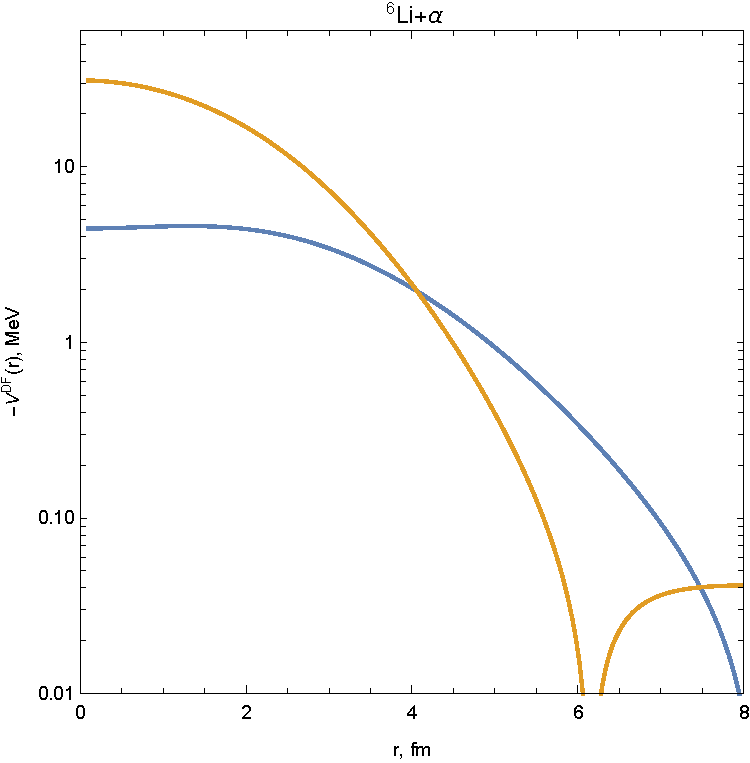
\includegraphics[scale=1]{li_df}
\decoRule
\caption{  \footnotesize  The folding potential $V^{DF}(r)$ in the framework of the three-body model. The potential is for the interaction of the $\alpha$ particle with the constituents of \li.
}
\label{li_df}
\end{figure}

The results of calculating the differential cross section of elastic collision of the $ \alpha $ + \li system are shown in Fig. \ref{li_elastic}~$a)$.
 The cross section based on the folding potential (DF-\li), represented by the blue curve, is in better agreement than the potential (WS1-\li) taken from \cite{oganessian1999dynamics}, which is shaped like the Woods-Saxon potential. 
 The proof comes from the value of the $\chi^2$ test for each potential. 
 The potential parameters and $\chi^2$ values are listed in Tab. \ref{tab:he_elastic}.
 The \li structure is very similar to the \he structure. Therefore, as in the case of \he, the calculations made in the framework of the OM are well described only at the forward scattering angles. 
 Differential cross sections belonging to the backward angles have the character of another mechanism - the transfer of $d$ inside \li. 
 How exactly this subsystem is transferred will be discussed in the next section devoted to elastic transfer for the $ \alpha$ + \he reaction.

\begin{figure}
\centering
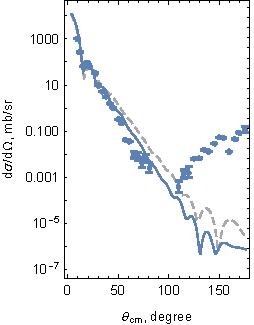
\includegraphics[scale=1.0]{li_elastic}
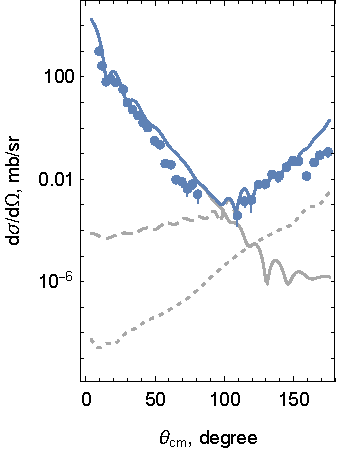
\includegraphics[scale=0.8]{li_elastic_transfer}\\
$~~~~~~a)~~~~~~~~~~~~~~~~~~~~~~~~~~~~~~~b)$
\decoRule
\caption{  \footnotesize  $a)$ The differential cross section of the elastic scattering of \li by $\alpha$-particles at $E_{lab} = 166 MeV$ with the different potentials: the double folding potential DF-\li (blue solid), the WS1-\li  (gray dashed) \cite{oganessian1999dynamics}. $b)$ The cross sections of the elastic transfer reaction are represented in terms of the transfer mechanisms: elastic scattering (solid gray), simultanious transfer of $d$ (gray dashed), sequential transfer of $2N$ (dotted) and their coherent sum (solid blue). Experimanetal data taken from \cite{oganessian1999dynamics}.
}
\label{li_elastic}
\end{figure}

Potential WS1-\li describes the experimental data not so much better than it was expected from the source taken \cite{oganessian1999dynamics}.
 It is possible that an error was overlooked at the typing stage for the publisher. It should be noted that omissions in our calculations for elastic scattering $\alpha$ + \li are excluded, since the approach perfectly reproduces the theoretical curves of the potential WS1-\he and WS2-\he for elastic scattering $\alpha$ + \he exactly the same as it looks in its own source. 
 
 It should be noted that the corresponding double folding potential  for the elastic scattering $\alpha$ + \li  reaction depends only on two parameters adjusted to the experimental data.



\subsection{Elastic transfer}
An increase in the cross section for the elastic scattering $\alpha$ + \li  reaction starting from 90$^\circ$ suggests the existence of additional reaction mechanisms.
 In this case, in order to register the same particle as the elastically scattered projectile, a deuteron particle must be transferred to the target at angles above 90$^\circ$. 
 That is, the incident particle \li transfers its deuteron to the $\alpha$-target. Then, the remaining alpha particle of \li continues its path, while the newly formed nucleus \li flies in the opposite direction according to the law of momentum conservation. 
 In particular, the presence of a deuteron transfer mechanism is not excluded. 
 These transfer mechanisms are shown schematically in Fig \ref{li_transfer_scheme}.

As in the case of \he, calculations for obtaining the differential cross section of the elastic transfer were carried out within the framework of the CRC method. For the input and output channels the double folding potential was taken, and for the intermediate channel the optical potential with global optical parametrizations for $\alpha$ particles \cite{avrigeanu1994global}  was chosen. Preliminary calculations have shown that the cross sections depend weakly on the selected potential for the intermediate channel.
The sequential transfer of two nucleons is shown by gray dotted curves, their simultaneous transfer by dashed gray curves, the elastic scattering cross section by solid gray curves, and, finally, their coherent sum is shown as a blue solid curve. 
The wave function of the bound states was chosen by fitting the potential depth to the binding energy of the composite systems. 
In particular, the binding energy of one neutron with $^5$Li was 5.663 MeV, as neutron with $^5$He taken 0.9 MeV, and as $d$ with  $\alpha$  taken 1.474 MeV. 
The differential cross section for this reaction is determined using the same formula \ref{eq:he_cs}.

\begin{figure}[tp!]
\centering
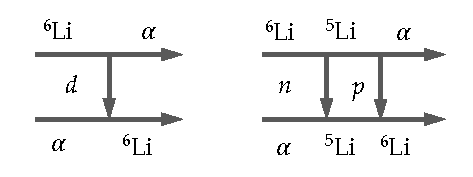
\includegraphics[scale=1]{li_transfer_scheme}
\decoRule
\caption{  \footnotesize  Schematic representation of the elastic transfer nuclear reaction, on the left - the simultaneous transfer of two nucleons, on the right - the sequential transfer of two nucleons.
}
\label{li_transfer_scheme}
\end{figure}

The results of calculations for elastic transfer are shown in Fig. \ref{li_elastic}.$b)$. 
The mechanism of elastic collision in the reaction of $\alpha$ + \li   prevails over other mechanisms at the forward scattering angles. 
However, starting from 90$^\circ$ we see that the main contribution to the cross section is caused by the simultaneous transfer of two nucleons of  \li, that is, the deuteron. 
The difference from the reaction $ \alpha $ + \he, where two nucleons are transferred, the reaction $\alpha $ + \li consists reaction of the deuteron transfer, which has spin $S(d)=1$, therefore, and also in the spin structure of the composite nucleus \li = $ \alpha + d $. That is, according to the law of conservation of moments and parity, a deuteron can be transferred by $2S1$ and $2D1$ configurations.

Calculations on the cross section showed that the cross section with the $2S1$ wave has an oscillatory character, as in the case with the elastic transfer reaction $\alpha$ + \he, then with the $2D1$ wave the cross section takes a smooth form. 
The SA for the $2S1$ configuration of the deuteron in \li was taken $ \mathcal {A}^{10} _ {2S1} \simeq 0.7 $, and for the $2D1$ configuration of the transferred deuteron $ \mathcal{A}^ {10}_{2D1} \simeq 0.5 $, considering that this wave has a much smaller contribution to the structure \li (see, Tab. \ref{tab:variational_data}). Therefore, the resulting section is more or less smooth compared to the case with the elastic transfer reaction $\alpha$ + \he.
As for the sequential transfer of the $d$ system, it has a contribution much less than the simultaneous transfer by one order of magnitude. This is when first neutron is transferred then proton. And the reverse order of transfer is greatly underestimated due to the Coulomb repulsion of proton with the $\alpha$-projectile.

\clearpage




\chapter{Beryllium-9}
\section{The d + $^9$Be nuclear reactions}

\subsection{The elastic channel}
The DF potential was calculated using the effective M3Y-Paris nucleon-nucleon potential and the nuclear-matter-densities of projectile and target nuclei. In order to calculate the ${}^9$Be matter distribution we applied the $\alpha+\alpha+n$ three-body model (for more details, see Ref.~\cite{urazbekov2016}), while the matter density distribution of the deuteron projectile was chosen to be of the form
\begin{equation}
\rho\left( \tfrac{1}{2}r \right) =\int \vert \Psi (\textbf{r}) \vert ^2 d \Omega_r.
\end{equation}

For convenience, in the OM and CC (CRC) calculations the potentials have been fitted by means of the sum of three Woods-Saxon potentials:
\begin{eqnarray}
V^V(R) =  \sum_{i=1}^{3} V^i f^{R_i, a_i}(R), \\
 f^{R_V,a_V}(R)=\frac{1}{1+exp{\frac{R-R_V}{a_V}}}.
\end{eqnarray}

\begin{figure}[bp!]
\centering
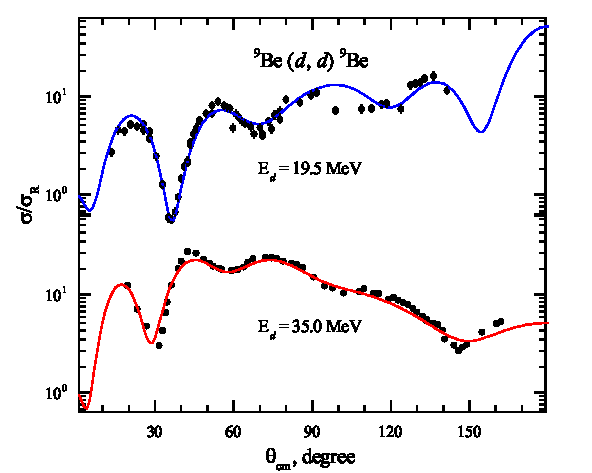
\includegraphics[width=8.2cm]{dbe_fig3.pdf}
\decoRule
\caption{ \label{dbe_fig3} \footnotesize The angular distribution of elastic scattering data of $d$ from ${}^9$Be at laboratory energy 19.5~MeV in comparison with theoretical calculations within the OM (solid curve). }
\end{figure}

The parameters of the imaginary part of the optical potential were obtained by fitting the theoretical cross sections to the experimental data at 19.5 MeV and 35 MeV incident energies. As a starting point, the same parameterizations of the real part were used. The obtained potential parameters after fitting are listed in Table~\ref{dbe_potpar} for both 19.5 MeV and 35.0 MeV incident energies.

The comparison of the results of the theoretical calculations with  the measured data for elastic scattering at 19.5 MeV and 35.0 MeV energies are plotted in Fig.~\ref{dbe_fig3}. 
The cross sections obtained in the framework of the OM with the DF potential are shown as solid curves. 
Theoretical results obtained by means of the OM give an excellent agreement, $\chi^2\approx2.5$, with the experimental data. The  parameters of  parameterized double-folding potential are listed in Table \ref{dbe_potpar}. 

\begin{table*}[bp]
\footnotesize
\caption{\label{dbe_potpar} \footnotesize Parameterized double-folding potentials of the $d$+$^9$Be system used in the OM, CC and DWBA calculations.}
\begin{tabular*}{\textwidth}{ll@{\extracolsep{\fill}}llllllllll}
\toprule
E$_d$, & i & V$_0$, & r$_v^{a}$, & a$_v$, & W$_0$, & r$_w^{a}$, & a$_w$, & V$_0^{SO}$, & N$_R$, & r$_C^{a}$, & $\chi^2/N$ \\
MeV   &   & MeV   & fm    & fm    & MeV   & fm    & fm    & MeV        &       & fm   						& \\ \midrule
19.5  & 1 & 6.18  & 0.328 & 0.308 & 3.99  & 0.328 & 0.127 & 3.275      & 1.22  & 0.809 			& 	2.490	\\
      & 2 & 70.97 & 0.746 & 0.831 & 25.50 (17.5$^{b}$) & 0.746 & 0.766 &            &       &    						&   \\
      & 3 & 0.605 & 1.491 & 1.724 & 0.924 & 1.491 & 2.238 &            &       &   							&    \\ \midrule
35.0  & 1 & 5.941 & 0.328 & 0.308 & 7.07  & 0.612 & 0.108 & 3.275      & 1.17  & 0.809 			&	2.503\\
      & 2 & 68.68 & 0.746 & 0.831 & 22.50 (17.5$^{b}$)& 0.838 & 0.731 &            &       &       						&\\
      & 3 & 0.58  & 1.491 & 1.724 & 0.999 & 1.377 & 1.856 &            &       &      							& \\ \bottomrule
\end{tabular*}
\scriptsize
$^{a}$ Radii are defined as $R_i = r_i \left( A^{1/3}_P+A^{1/3}_T \right)$.  \\
$^{b}$ The values are used in CRC calculations. \\
\end{table*}


\subsection{Inelastic scattering}
The CC and DWBA approaches have been applied to analyse the measured inelastic scattering data corresponding to the ${}^9$Be($5/2^-, 2.43$ MeV) excitation. Calculations were performed employing the FRESCO code \cite{fresco} and the DWUCK5 code \cite{kunz} which are available in the NRV knowledge-base \cite{nrv}.

In order to describe the measured experimental data one has to consider the ${}^9$Be target having a quadrupole deformation. Thus, the ${}^9$Be spectrum consists of the rotational band including the  $3/2^-$ ground state, $5/2^-$ state at 2.43 MeV and $7/2^-$ state at 6.38 MeV. Couplings to these states were taken into account within the coupled-channel approach. The spin reorientations were also taken into account. The coupling interaction has the usual form:
\begin{equation}
V_\lambda(R)=-\beta_\lambda R_V \left|\frac{d V^V}{dR}\right| - i \beta_\lambda R_W \left|\frac{d W^D}{dR}\right|,
\end{equation}
where $\beta_\lambda$ is the deformation parameter of $\lambda$ multipole describing the target-nucleus form. Here, we neglect as usual the contribution of the Coulomb interaction.

\begin{figure}[tp]
\centering
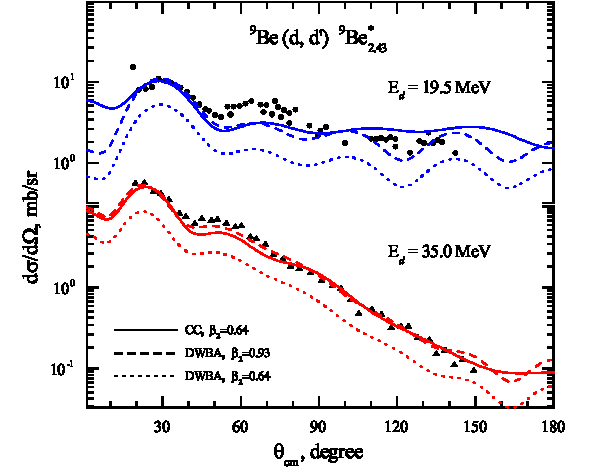
\includegraphics[width=8.2cm]{dbe_fig4.pdf}
\decoRule
\caption{\label{dbe_fig4} \footnotesize The cross sections of inelastic scattering ${}^9$Be($d,d$)$^9$Be* (E$_{exc}$=2.43 MeV) at laboratory energies 19.5 MeV (full circle) and 35 MeV (full triangle). Theoretical curves are described in the text.}
\end{figure} 


\begin{figure}[bp]
\centering
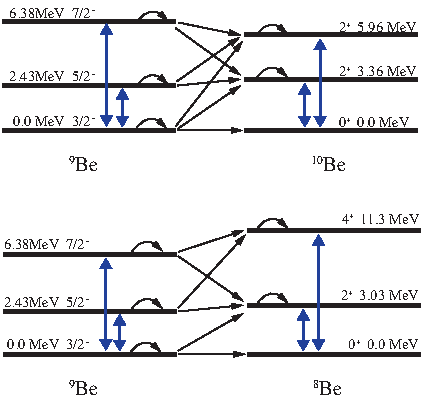
\includegraphics[scale=0.85]{dbe_fig5.pdf}
\decoRule
\caption{ \label{dbe_fig5} \footnotesize The target coupling schemes in the ${}^9$Be($d,p$)$^{10}$Be (upper) and the ${}^9$Be($d,t$)$^8$Be (lower) nuclear reactions. The bold two-headed arrows indicate E$\lambda$ transitions. The spin re-orientation effects are indicated as back-pointing arrows.}
\end{figure} 

The calculated cross sections for inelastic scattering to the $5/2^-$ state at 2.43 MeV are shown in Fig.~\ref{dbe_fig4}. The solid curves correspond to the results obtained within the CC approach, while the dashed and dotted curves were obtained within the DWBA approach using  different values of the deformation parameter $\beta_2$. The used potential parameters are listed in Table~\ref{dbe_potpar}.


All the results in Fig.~\ref{dbe_fig4} are in good agreement with the experimental data, except for the cross sections around 60$^\circ$ at 19.5 MeV incident energy. The quadrupole deformation parameter $\beta_2 = 0.64$ extracted within the coupled-channel model is consistent with the previous studies \cite{lukyanov2014study, harakeh1980strong}.

In the case of DWBA calculations, one uses the DF potential (see Table~\ref{dbe_potpar}) for both the entrance and the exit channels. The DWBA angular distributions very well reproduce the structure of experimental data but clearly underestimate them when the deformation parameter $\beta_2 = 0.64$ is used (see the dotted curves in Fig.~\ref{dbe_fig4}). In order to get the best fit the deformation parameter must be increased up to $\beta_2 = 0.93$, which is quite close to the values reported in previous studies (see, for example, \cite{bodek1989, votava1973}).

Thus, one may confirm that channel coupling and the effects of spin reorientation enhance the cross section that results in the reduction of the deformation parameter. However, the DWBA approach takes into account only first-order contributions to the transition amplitude. In particular, it also describes only general features of the angular distributions and overestimates the deformation parameter in order to compensate the difference between the experimental data and the DWBA cross sections.

\subsection{One-nucleon transfer reactions }

The one-neutron pick-up ${}^9$Be($d,t$)${}^8$Be and stripping ${}^9$Be($d,p$)${}^{10}$Be reactions were analyzed here within the framework of  the Coupled Reaction Channels (CRC).

The double-folding potential given in Table \ref{dbe_potpar} was used in the CRC calculations for the entrance channel and the global optical parameterizations from Ref. \cite{globalProton, globalTriton} were used for the exit channels. The coupling schemes of target and daughter nuclei for the ${}^9$Be($d,p$)${}^{10}$Be and ${}^9$Be($d,t$)${}^8$Be  reactions  are illustrated in Fig. \ref{dbe_fig5}. The states of ${}^{10}$Be, $2^+_{1}$ and $2^+_{2}$, as well as the low-lying excited states of ${}^8$Be, $2^+$ and $4^+$, were included in the coupling scheme. Also, the schemes take into account the spin reorientations of states on the condition $J \neq 0$.

In order to construct the bound-state wave functions of the transferred particle in the entrance and exit channels, the common method, i.e. fitting the depth of the corresponding Woods-Saxon potential to the known binding energy, was employed. The reduced radius and diffuseness in this case are set to be $r = 1.25$ fm and $a$ = 0.65 fm, respectively. If the transfer takes place to a final unbound state, the depth of the potential for this state was adjusted to yield a binding energy equal to $-0.1$ MeV in accordance with the procedure used in Ref. \cite{harakeh1980strong}.

\begin{figure}[tp]
\centering
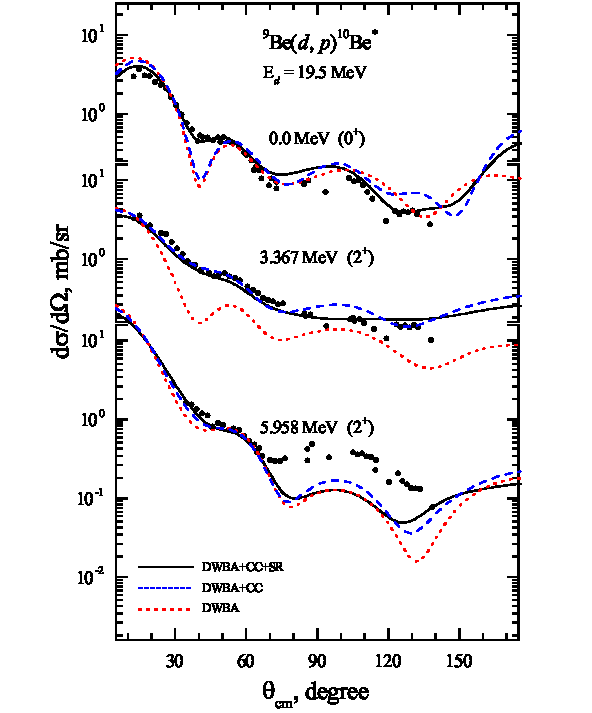
\includegraphics[scale=0.8]{dbe_fig6.pdf}
\decoRule
\caption{\label{dbe_fig6} \footnotesize Differential cross sections for the ${}^9$Be($d,p$)${}^{10}$Be$^*$ reactions at 19.5 MeV leading to different final states (labelled in the figure) in ${}^{10}$Be. The experimental data are shown in comparison with theoretical results obtained within the CRC method.}
\end{figure}

If the core and the composite nuclei have internal excitation energies, a renewed binding energy $BE^{\star}$ of the transferred particle is expressed by the formula:
\begin{equation} BE^{\star}=BE - E_{com}^*+E_{core}^* \end{equation}
where $BE$ $-$ the binding energy of the transferred particle, $E_{com}^*,~E_{core}^*~-$  excitation energies of the composite and  core nuclei, respectively.

\begin{figure}[tp]
\centering
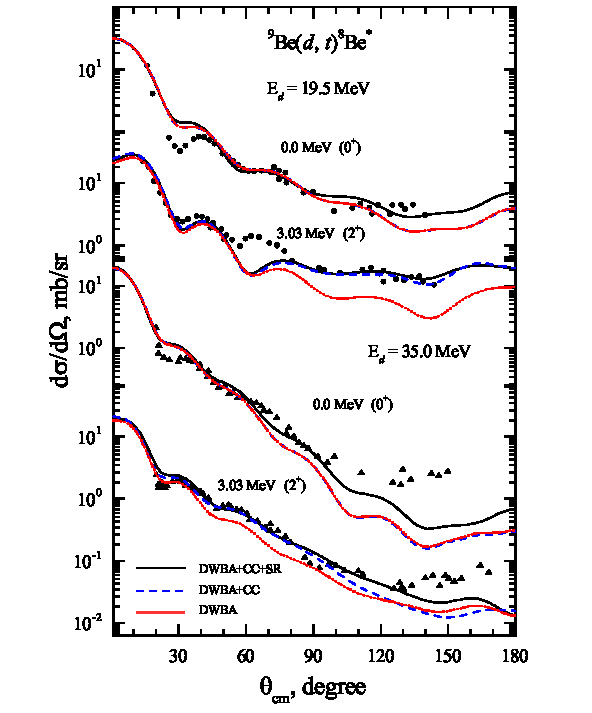
\includegraphics[scale=0.7]{dbe_fig7.pdf}
\decoRule
\caption{
\label{dbe_fig7}
\footnotesize Differential cross sections for the ${}^9$Be($d,t$)${}^{8}$Be$^*$ reactions at 19.5 and 35 MeV leading to different final states (labelled in the figure) in ${}^{8}$Be. The experimental data are shown in comparison with  theoretical results obtained within the CRC method.}
\end{figure}

The SA  $\mathcal{A}$ for the addition of a particle to a core with angular momentum $J_{core}$ to form a composite with $J_{com}$ is related to the matrix element of the creation operator~$\hat{a}^\dagger$:
%\cite{brown2017}:
\begin{eqnarray}\label{eq:SA}
\mathcal{A}_{Nlj} = \frac{\langle J_{com} \| \hat{a}^\dagger _{Nlj} \| J_{core}  \rangle}{\sqrt{2J_{com}+1}}
%= (-)^{j+J-J'} \frac{\langle J_{core}  \| \hat{a} _{NL_J} \| J_{com}  \rangle}{\sqrt{2J+1}}
\end{eqnarray}
where $Nlj$ is the set of particle quantum numbers. The spectroscopic amplitudes for one particle states were calculated by means of the $ANTOINE$ code \cite{antoine}  using the effective Cohen-Kurath interaction for $p$-shell nuclei \cite{cohen1965}. The calculated SA for the one-nucleon transfer reactions are listed in Table~\ref{dbe_SA}.

\begin{table*}[tp]
\footnotesize
\caption{\label{dbe_SA} \footnotesize Spectroscopic amplitudes used in CRC calculations for the Composite = Core + Nucleon system. The one-nucleon SA have been calculated by means of the $ANTOINE$ code \cite{antoine}. The alpha spectroscopic amplitudes were taken from  \cite{volya, volya2017}. }
\begin{tabular*}{\textwidth}{@{\extracolsep{\fill}}llllllrl@{\extracolsep{\fill}}llllllr@{\extracolsep{\fill}}}
\toprule
Com & 2J$_{1}$ & Core & 2J$_{2}$ & N & 2J & SA &    & Com & 2J$_{1}$ & Core & 2J$_{2}$ & N & 2J & SA      \\
\midrule 
$^9$Be  & 3  & ${}^8$Be   & 0   & $n$       & 3   & $-$0.761 &  & ${}^9$Be  & 3  & ${}^8$Li   & 2$_1$    & $p$       & 1   & $-$0.444  \\
$^9$Be  & 3  & ${}^8$Be   & 4   & $n$       & 3   & 0.816  &  & ${}^9$Be  & 3  & ${}^8$Li    & 6   & $p$       & 3   & $-$0.592  \\
$^9$Be  & 3  & ${}^8$Be   & 4   & $n$       & 1   & $-$0.242 &  & ${}^9$Be  & 3  & ${}^8$Li    & 2$_2$   & $p$       & 3   & $-$0.236  \\
$^9$Be  & 5  & ${}^8$Be   & 4   & $n$       & 3   & 0.986  &  & ${}^9$Be  & 3  & ${}^8$Li    & 2$_2$   & $p$       & 1   & 0.036   \\
$^9$Be  & 5  & ${}^8$Be   & 4   & $n$       & 1   & $-$0.417 &  & ${}^9$Be  & 5  & ${}^8$Li    & 4   & $p$       & 3   & 0.593   \\
$^9$Be  & 5  & ${}^8$Be   & 8   & $n$       & 3   & $-$0.374 &  & ${}^9$Be  & 5  & ${}^8$Li    & 4   & $p$       & 1   & 0.515   \\
$^9$Be  & 7  & ${}^8$Be   & 4   & $n$       & 3   & $-$0.457 &  & ${}^9$Be  & 5  & ${}^8$Li   & 2$_1$    & $p$       & 3   & $-$0.672  \\
$^9$Be  & 7  & ${}^8$Be   & 8   & $n$       & 3   & 0.919  &  & ${}^9$Be  & 5  & ${}^8$Li    & 6   & $p$       & 3   & $-$0.571  \\
$^9$Be  & 7  & ${}^8$Be   & 8   & $n$       & 1   & $-$0.429 &  & ${}^9$Be  & 5  & ${}^8$Li    & 6   & $p$       & 1   & $-$0.171  \\
$^8$Be  & 0  & ${}^7$Li   & 3   & $p$       & 3   & $-$1.204 &  & ${}^9$Be  & 5  & ${}^8$Li    & 2$_2$   & $p$       & 3   & 0.200     \\
$^8$Be  & 0  & ${}^7$Li   & 1   & $p$       & 1   & 0.736  &  & ${}^9$Be  & 7  & ${}^8$Li    & 4   & $p$       & 3   & $-$0.323  \\
$^8$Be  & 4  & ${}^7$Li   & 3   & $p$       & 3   & $-$0.748 &  & ${}^9$Be  & 7  & ${}^8$Li    & 6   & $p$       & 3   & $-$0.899  \\
$^8$Be  & 4  & ${}^7$Li   & 3   & $p$       & 1   & $-$0.612 &  & ${}^9$Be  & 7  & ${}^8$Li    & 6   & $p$       & 1   & $-$0.564  \\
$^8$Be  & 4  & ${}^7$Li   & 1   & $p$       & 3   & 0.667  &  & ${}^7$Li  & 3  & ${}^6$Li   & 2   & $n$       & 3   & 0.657   \\
$^8$Be  & 4  & ${}^7$Li   & 7   & $p$       & 3   & 0.624  &  & ${}^7$Li  & 3  & ${}^6$Li   & 2   & $n$       & 1   & $-$0.538  \\
$^8$Be  & 4  & ${}^7$Li   & 5$_2$   & $p$       & 3   & 0.079  &  & ${}^7$Li  & 3  & ${}^6$Li   & 6   & $n$       & 3   & 0.744   \\
$^8$Be  & 4  & ${}^7$Li   & 5$_2$   & $p$       & 3   & $-$0.146 &  & ${}^7$Li  & 3  & ${}^6$Li   & 4   & $n$       & 3   & $-$0.032  \\
$^8$Be  & 8  & ${}^7$Li   & 7   & $p$       & 3   & 0.864  &  & ${}^7$Li  & 3  & ${}^6$Li   & 4   & $n$       & 1   & 0.399   \\
$^8$Be  & 8  & ${}^7$Li   & 7   & $p$       & 1   & 0.687  &  & ${}^7$Li  & 1  & ${}^6$Li   & 2   & $n$       & 3   & $-$0.925  \\
$^8$Be  & 8  & ${}^7$Li   & 5$_2$   & $p$       & 3   & 0.374  &  & ${}^7$Li  & 1  & ${}^6$Li   & 2   & $n$       & 1   & 0.197   \\
$^8$Li  & 4  & ${}^7$Li   & 3   & $n$       & 3   & $-$0.988 &  & ${}^7$Li  & 1  & ${}^6$Li   & 4   & $n$       & 3   & $-$0.555  \\
$^8$Li  & 4  & ${}^7$Li   & 3   & $n$       & 1   & 0.237  &  & ${}^7$Li  & 7  & ${}^6$Li   & 6   & $n$       & 3   & $-$0.936  \\
$^8$Li  & 4  & ${}^7$Li   & 1   & $n$       & 3   & 0.430   &  & ${}^7$Li  & 7  & ${}^6$Li   & 6   & $n$       & 1   & 0.645   \\
$^8$Li  & 4  & ${}^7$Li   & 7   & $n$       & 3   & $-$0.496 &  & ${}^7$Li  & 7  & ${}^6$Li   & 4   & $n$       & 3   & $-$0.456  \\
$^8$Li  & 4  & ${}^7$Li   & 5   & $n$       & 3   & $-$0.665 &  & ${}^7$Li  & 5$_2$  & ${}^6$Li   & 2   & $n$       & 3   & $-$0.650   \\
$^8$Li  & 4  & ${}^7$Li   & 5$_2$   & $n$       & 1   & $-$0.275 &  & ${}^7$Li  & 5$_2$  & ${}^6$Li   & 6   & $n$       & 3   & 0.732   \\
$^8$Li  & 2$_1$  & ${}^7$Li   & 3   & $n$       & 3   & 0.567  &  & ${}^7$Li  & 5$_2$  & ${}^6$Li   & 6   & $n$       & 1   & 0.549   \\
$^8$Li  & 2$_1$  & ${}^7$Li   & 3   & $n$       & 1   & 0.351  &  & ${}^7$Li  & 5$_2$  & ${}^6$Li   & 4   & $n$       & 3   & 0.200     \\
$^8$Li  & 2$_1$  & ${}^7$Li   & 1   & $n$       & 3   & 0.905  &  & ${}^7$Li  & 5$_2$  & ${}^6$Li   & 4   & $n$       & 1   & $-$0.114  \\
$^8$Li  & 2$_1$  & ${}^7$Li   & 1   & $n$       & 1   & 0.331  &  & ${}^6$Li  & 2  & $d$     & 2   & $\alpha$     & 0   & 0.907  \\
$^8$Li  & 2$_1$  & ${}^7$Li   & 5$_2$   & $n$       & 3   & 0.767  &  & ${}^6$Li  & 2  & $d$     & 2   & $\alpha$     & 4   & 0.077   \\
$^8$Li  & 6  & ${}^7$Li   & 3   & $n$       & 3   & 0.581  &  & ${}^6$Li  & 6  & $d$     & 2   & $\alpha$     & 4   & 0.943   \\
$^8$Li  & 6  & ${}^7$Li   & 5$_2$   & $n$       & 3   & $-$0.660  &  & ${}^6$Li  & 6  & $d$     & 2   & $\alpha$     & 8   & 0.028   \\
$^8$Li  & 6  & ${}^7$Li   & 5$_2$   & $n$       & 1   & $-$0.541 &  & ${}^6$Li  & 4  & $d$     & 2   & $\alpha$     & 4   & 0.929   \\
$^8$Li  & 6  & ${}^7$Li   & 7   & $n$       & 3   & 0.973  &  & ${}^9$Be  & 3  & ${}^5$He   & 3   & $\alpha$     & 0   & $-$0.925  \\
$^8$Li  & 6  & ${}^7$Li   & 7   & $n$       & 1   & $-$0.404 &  & ${}^9$Be  & 3  & ${}^5$He   & 3   & $\alpha$     & 4   & 0.784   \\
$^8$Li  & 2$_2$  & ${}^7$Li   & 3   & $n$       & 3   & $-$0.617 &  & ${}^9$Be  & 5  & ${}^5$He   & 3   & $\alpha$     & 4   & 0.974   \\
$^8$Li  & 2$_2$  & ${}^7$Li   & 3   & $n$       & 1   & $-$0.841 &  & ${}^9$Be  & 5  & ${}^5$He   & 3   & $\alpha$     & 8   & $-$0.260   \\
$^8$Li  & 2$_2$  & ${}^7$Li   & 1   & $n$       & 3   & 0.178  &  & ${}^9$Be  & 7  & ${}^5$He   & 3   & $\alpha$     & 4   & 0.882   \\
$^8$Li  & 2$_2$  & ${}^7$Li   & 1   & $n$       & 1   & 0.331  &  & ${}^9$Be  & 7  & ${}^5$He   & 3   & $\alpha$     & 8   & $-$0.737  \\
$^8$Li  & 2$_2$  & ${}^7$Li   & 5   & $n$       & 3   & 0.231  &  & ${}^7$Li  & 3  & $t$     & 1   & $\alpha$     & 1   & 0.970       \\
$^9$Be  & 3  & ${}^8$Li    & 4   & $p$       & 3   & $-$0.947 &  & ${}^7$Li  & 1  & $t$     & 1   & $\alpha$     & 1   & 0.961       \\
$^9$Be  & 3  & ${}^8$Li    & 4   & $p$       & 1   & $-$0.319 &  & ${}^7$Li  & 7  & $t$     & 1   & $\alpha$     & 3   & 0.952       \\
$^9$Be  & 3  & ${}^8$Li    & 2$_1$   & $p$       & 3   & 0.454  &  & ${}^7$Li  & 5$_2$  & $t$     & 1   & $\alpha$     & 3   & 0.223  \\
\bottomrule
\end{tabular*}
\end{table*}

Angular distributions of the ${}^9$Be($d,p$)${}^{10}$Be nuclear reaction at E$_d$=19.5 MeV are shown in comparison with the theoretical curves  calculated in the framework of the CRC method in Fig. \ref{dbe_fig6}.

In order to study the couplings of the input  channels, the outputs  were fixed using the deformation parameter of $^8$Be from Ref. \cite{rocca2018}, and for $^{10}$Be from Ref. \cite{harakeh1980strong}. 
The direct transition from the ground state is indicated by the dotted line (DWBA). 
The contributions of the transitions from excited states (CC), and from spin reorientations (SR) are indicated by dashed and solid lines, respectively.
During the analysis, it was found that spin reorientation has a significant contribution in the $p$ + $^{10}$Be$_{gs}$ channel, especially in the range of 40-60 degrees. 

It is interesting to note that we managed to describe within the CRC method the differential cross section of the ${}^9$Be($d,p$)${}^{10}$Be$_{gs}$ reaction at all scattering angles, including the range 40$^\circ$-60$^\circ$, where they were not covered in Refs. \cite{galanina2012, bodek1989}.
 
An appreciable contribution of the \begin{small}
$3/2^- \rightarrow 2^+_1,~5/2^- \rightarrow 2^+_1,~7/2^-\rightarrow 2^+_1$
\end{small} transitions was observed in the $p$~+~$^{10}$Be$_{3.37}$ channel in the entire range of scattering angles. 
In the cross section of the  $p$~+~$^{10}$Be$_{5.96}$ channel, the theoretical calculation underestimates the experimental data starting from 70$^\circ$. Possibly, other higher excited states of $^9$Be should be taken into account.

Figure \ref{dbe_fig7} displays the cross sections of the ${}^9$Be($d,t$)${}^{8}$Be nuclear reaction at both 19.5 MeV and 35 MeV incident energies. As in the case of the ($d,p$) reactions, the ($d,t$) reactions also show the strong channel-coupling effects. We see a manifestation of spin-reorientation effects in the $t$+$^8$Be$_{gs}$ channels and a significant contribution of the  \begin{small}
$3/2^- \rightarrow 2^+,~ 5/2^- \rightarrow 2^+,~ 7/2^-\rightarrow 2^+$
\end{small} transitions in the $t$+$^8$Be$_{3.03}$ channel.
Disagreements around 30$^\circ$ in the $t$+$^8$Be$_{gs}$ channel for both 19.5 MeV and 35 MeV incident energies and around 60$^\circ$ in the $t$+$^8$Be$_{3.03}$ channel for 19.5 MeV incident energy are possibly caused by the uncertainty in the $t$+$^8$Be interaction potential.

Theoretical calculations made within the CRC method show, in general, good agreement with the experimental data for both ($d,p$)  and ($d,t$) reactions.
The analysis showed strong coupling effects in both entrance and exit channels. The effects of such couplings were also emphasized in Refs. \cite{harakeh1980strong, rudchik2016}.

\subsection{Cluster-transfer reaction}
Differential cross sections for the nuclear reaction ${^9}$Be($d,\alpha$)${}^7$Li are of particular interest. This is due to the specific behaviour of the cross section at large scattering angles, which indicates a ${}^5$He cluster transfer. In addition, the cross section calculated within the DWBA approach underestimates the data even at forward scattering angles. Therefore, in order to understand the difference between theory and experiment, the following transfer mechanisms are suggested (see Fig. \ref{dbe_fig9}):
\begin{itemize}
\item[$-$] direct transfer of heavy clusters $d$ and ${}^5$He;
\item[$-$] sequential two-step transfer of $n$-$p$, $p$-$n$, $n$-$\alpha$ and $\alpha$-$n$;
\end{itemize}


\begin{figure}[tp]
\centering
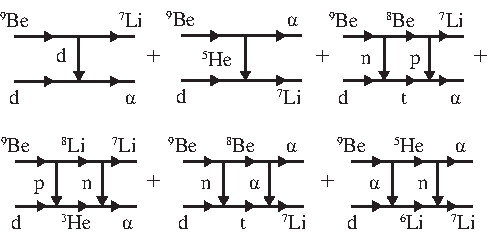
\includegraphics[width=8.2cm]{dbe_fig9.pdf}
\decoRule
\caption{\label{dbe_fig9} \footnotesize The scheme illustrates the reaction mechanisms taken into account in CRC calculations of the cross sections for ${}^9$Be($d,\alpha$)${}^7$Li reaction.}
\end{figure}


The resulting differential cross section for the ${^9}$Be($d$,$\alpha$)${}^7$Li reaction has the form of a coherent sum of two amplitudes
\begin{equation}
\frac{d\sigma}{d\Omega}(\theta) =\vert f_{I}(\theta) + f_{II}(\theta) \vert ^2,
\end{equation}
where the amplitude
\begin{equation} \label{eq:ampl1}
f_{I}(\theta)=f_{{}^5\textrm{He}}(\pi - \theta) + f_{n\textrm{-}\alpha}(\pi - \theta) + f_{\alpha\textrm{-}n}(\pi - \theta)
\end{equation}
describes the transfer of the heavy ${}^5$He-cluster and sequential two-step transfer of n-$\alpha$ and $\alpha$-n, and the amplitude
\begin{equation} \label{eq:ampl2}
f_{II}(\theta)=f_{d}(\theta) + f_{n\textrm{-}p}( \theta) + f_{p\textrm{-}n}(\theta)
\end{equation}
corresponds to the deuteron pick-up and sequential two-step transfer of $n$-$p$ and $p$-$n$.


\begin{figure*}[tp]
\centering
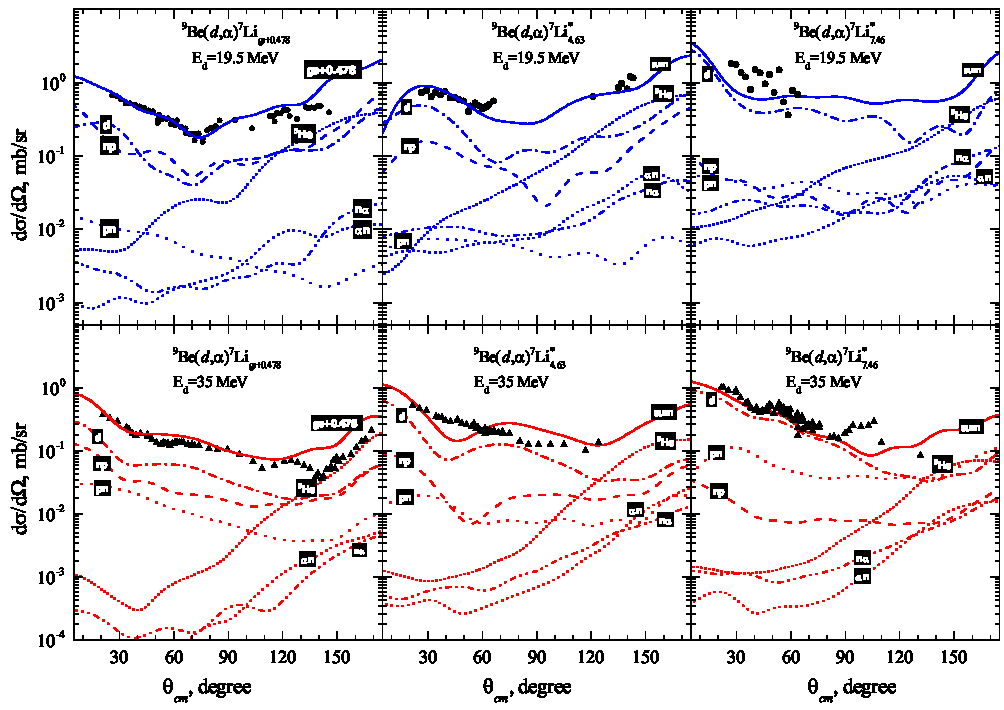
\includegraphics[scale=0.8]{dbe_fig8.pdf}
\decoRule
\caption{ \footnotesize Differential cross sections for the ${}^9$Be($d$,$\alpha$)${}^7$Li reactions measured at 19.5 MeV and 35 MeV energy with the ${}^{7}$Li observed in the ground or low-lying excited states in the exit channels.}
\label{dbe_fig8}
\end{figure*}	


The DF potential (see Table~\ref{dbe_potpar}) for the entrance channel and global optical potential parameterizations from Refs. \cite{globalTriton, globalAlpha, global6Li} for intermediate and exit channels were used in the analysis.
The prior form for the first coupling and the post form for the second coupling were chosen for two-step transfer reactions in order to avoid the non-orthogonal terms in the calculations of transition amplitudes.

%Important ingredients of the CRC method are the spectroscopic amplitudes of the composite configurations in the entrance, exit and intermediate states. In order to calculate the one nucleon spectroscopic amplitudes we applied the \textit{ANTOINE} code \cite{antoine} that reproduces the excitation functions of all p-shell nuclei well.

The spectroscopic amplitudes of the $d$ and ${}^5$He clusters were taken from Ref. \cite{fiveSA}, while the alpha-cluster spectroscopic amplitudes given in Table~\ref{dbe_SA} were provided by Dr. A. Volya within the method reported in Ref. \cite{volya2017}.

The calculated cross sections are shown in Fig.~\ref{dbe_fig8} with the $\alpha$-particle angular distributions formed in the ${}^9$Be(d,$\alpha$)${}^7$Li$^*$ reaction at incident energies of 19.5 and 35 MeV and corresponding to the low-lying excitation of the ${}^7$Li nucleus in the exit channels. The transfer of the deuteron (dash-dotted curve) provides the dominant contribution in all the channels. Despite the fact that the spectroscopic amplitude of the deuteron $\mathcal{A}_{1{D}_3}=0.558$ in the ${}^9$Be nucleus is not of great importance, a noticeable cross section is due to the large value of the deuteron spectroscopic amplitude $\mathcal{A}_{1{S}_1}=1.732$  of ${}^4$He.

The angular distribution of deuteron transfer has a significant cross section also at the backward scattering angles, which is mainly caused by the contribution of the $D$ wave. This symmetrical behaviour of the cross section of $D$ waves is very similar to the cross section of evaporation residues. Tanaka \textit{et al} \cite{tanaka1978} analyzed the role of the compound process in ${}^9$Be($d,\alpha$)${}^7$Li reaction and claimed the domination of the compound nucleus channels at the energies of 12.17 MeV and 14.43 MeV. However, in Ref. \cite{bodek1989} the negligible contribution of the compound-nucleus mechanism was shown at 7 MeV using the DWBA analysis. In this regard, our theoretical results based on the CRC method show that there is no need to take into account the mechanism through the compound-nucleus formation at energies of 19.5 and 35.0 MeV.

Starting from scattering angle $\theta_{c.m.} =$ 120$^\circ$, the transfer of the ${}^5$He cluster, labeled as ${}^5$He in Fig. \ref{dbe_fig8}, has a predominant contribution in all channels. It should be noted that a similar result was reported earlier in Ref. \cite{bodek1989}. One-step transfer of the ${}^5$He cluster was also indicated as a dominant process by Jarczyk \textit{et al} \cite{jarczyk1996} in studying the ${}^{12}$C(${}^{11}$B,${}^6$Li)${}^{17}$O and ${}^{12}$C($d$,${}^7$Li)${}^{7}$Be reactions.

Using the CRC method, we are able to estimate the contribution of the sequential transfer of ${}^5$He, which was not studied before. Corresponding cross sections are shown in Fig.~\ref{dbe_fig8} as curves labeled $n\alpha$ and $\alpha n$.
It turned out that the $n$-$\alpha$ and $\alpha$-$n$ transfer processes provide indeed a contribution more than one order of magnitude smaller in comparison with the one-step ${}^5$He transfer. Nevertheless, it should be noted that the contribution of the $n$-$\alpha$ and the $\alpha$-$n$ transfer channels increases with the increase in the ${}^7$Li excitation energy, where they should not be ignored.

\begin{figure}%[tp]
\centering
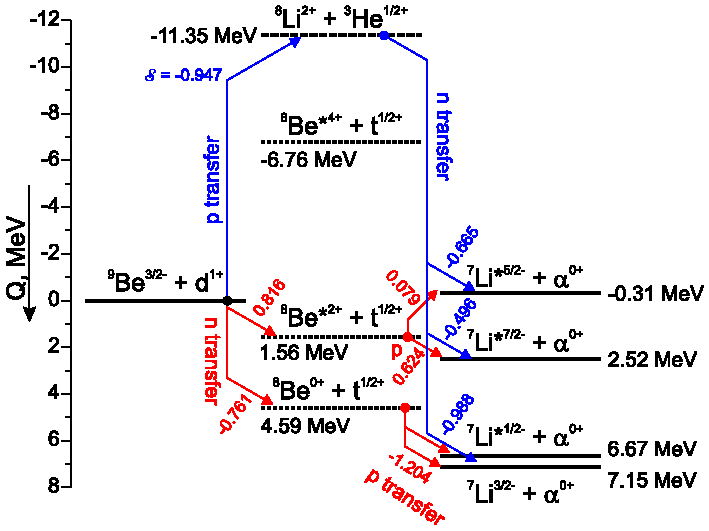
\includegraphics[width=8.2cm]{dbe_fig10.pdf}
\decoRule
\caption{\label{dbe_fig10} \footnotesize The scheme illustrates the energy balance of the different intermediate stages for the two-step mechanisms of ${}^9$Be($d,\alpha$)${}^7$Li transfer reaction. The $Q$-values for the different intermediate channels are shown near the corresponding lines. The numbers near the arrows correspond to the spectroscopic amplitudes of the heaviest reaction participants. For example, spectroscopic amplitude for the ${}^9$Be = ${}^8$Li + $p$ configuration is equal $\mathcal{A} = -0.947$.}
\end{figure}

The two-step $n$-$p$ transfer is another mechanism providing a noticeable contribution to the cross section. It is due to the prominent cluster structure of the ${}^9$Be nucleus having the weakly bound neutron. This structural feature explains also the weakness of the $p$-$n$ sequential transfer contribution to the cross section corresponding to the ${}^7$Li(g.s.) in the exit channel. However, with increasing the ${}^7$Li excitation energy these two mechanisms are interchanged in the significance of their contributions, as depicted by the curves in Fig.~\ref{dbe_fig8}, and the $p$-$n$ transfer begins to play a leading role, providing, in particular, almost 10 times larger contribution in the case of reaction at $E_{lab}$ = 35 MeV with ${}^7$Li$^*$(7.46 MeV) in exit channel.

In Fig.~\ref{dbe_fig10}, the possible scenarios for the $n$-$p$ and $p$-$n$ sequential transfer for the reaction under consideration are shown in respect to the $Q$-values. One may see that all the steps of the $n$-$p$ sequential transfer have positive $Q$-values, while the $p$-$n$ transfer goes through the intermediate channel ${}^8$Li + ${}^3$He that has a considerably negative $Q$-value. Together with the large values of the spectroscopic amplitudes (shown near to the arrows in Fig. \ref{dbe_fig10}), this explains the leading role of the ($d,t;t,\alpha$) mechanism in populating the ground state of ${}^7$Li in the exit channel.

\begin{figure}[tp]
\centering
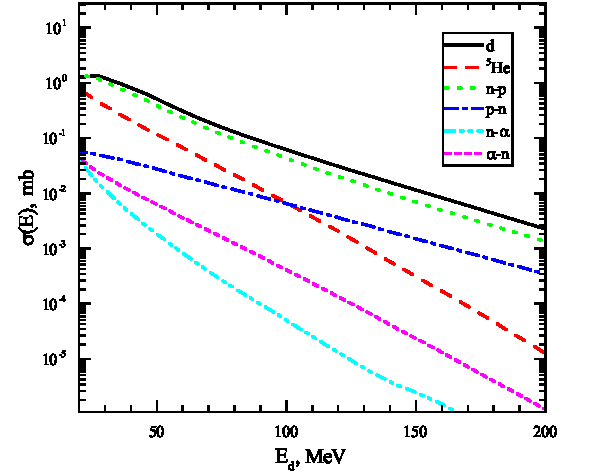
\includegraphics[width=8.2cm]{dbe_fig11.pdf}
\decoRule
\caption{\label{dbe_fig11} \footnotesize Contributions of the different mechanisms to the cross section of the ${}^9$Be($d,\alpha$)${}^7$Li$_{g.s.}$ reaction. See Fig.~\ref{dbe_fig9} for explanation of the curve notations.}
\end{figure}	

The situation becomes quite different in the case of the ${}^7$Li$^*$(5/2$^-$) in the exit channel. First, the population of this state through the $n$-$p$ transfer involves the ${}^9$Be~=~${}^8$Be$^*(2^+)$~+~$n$ intermediate configuration where the ${}^8$Be cluster has to be in the $2^+$ excited state. Note that the ${}^8$Be($0^+$) ground state is inappropriate because of angular-momentum-coupling mismatch in the entrance and exit configurations. Second, the extremely small spectroscopic amplitude of the ${}^8$Be$^*(2^+)$~=~${}^7$Li$^*(5/2^-)$~+~$p$ configuration, which is $\mathcal{A} = 0.079$, influences the transfer amplitude. These two factors lead to the suppression of the contribution of ($d,t;t,\alpha$) mechanism in population of the ${}^7$Li$^*$(5/2$^-$) state in the exit channel. Therefore, the $p$-$n$ sequential transfer prevails over the $n$-$p$ one. 

Figure \ref{dbe_fig11} shows the contributions of all the mechanisms mentioned above to the total cross section of the ${}^9$Be($d,\alpha$)${}^7$Li$_{g.s.}$ reaction (see Fig.~\ref{dbe_fig9}) as a function of the deuteron energy. One may conclude that mainly four mechanisms contribute to the cross section of this reaction. The transfer of the deuteron-cluster is the predominant channel at all collision energies. The sequential $n$-$p$ and $p$-$n$ transfers play a significant role at the high energies. The ${}^5$He-cluster transfer gives almost 20\% of the cross section at low energies and outdoes the sequential $p$-$n$ transfer in this energy domain. This allows us to claim that the configurations $n+^8$Be and $\alpha+{}^5$He provide noticeable contributions to the ground-state wave function of the ${}^9$Be nucleus. These conclusions agree well with the previous experimental studies \cite{brown2007, papka2007}.


\chapter*{Conclusion}   
\addchaptertocentry{Conclusion}


In the present work, the deuteron-induced reactions on a ${}^9$Be target have been studied at the collision energies 19.5 and 35 MeV.
The calculated double-folding potential has been applied successfully in describing the cross sections of elastic and inelastic scatterings, one-nucleon  transfer and cluster-transfer reactions.
  The deformation parameter for the transition \begin{small}
  $3/2^-\rightarrow5/2^-$
\end{small}  of ${}^9$Be has been determined.
 The strong coupling effects have been shown for the ($d,p$) and ($d,t$) one-nucleon transfer nuclear reactions.
 Furthermore, it was found that  in the ${}^9$Be($d$,$\alpha$)${}^7$Li nuclear reaction the ${}^5$He heavy cluster  is transferred mainly simultaneously, and the contribution of its sequential transfer is an order of magnitude lower.
 The importance of taking into account the mechanism of sequential transfer of the $n$-$p$ system has been revealed.
 Based on these observations from studying the interaction of the  deuteron with  $^9$Be, it can be concluded that the $^9$Be  nucleus has cluster structure.
 
%\include{Chapters/Chapter2} 
%\include{Chapters/Chapter3}
%\include{Chapters/Chapter4} 
%\include{Chapters/Chapter5} 

%----------------------------------------------------------------------------------------
%	THESIS CONTENT - APPENDICES
%----------------------------------------------------------------------------------------

\appendix % Cue to tell LaTeX that the following "chapters" are Appendices

% Include the appendices of the thesis as separate files from the Appendices folder
% Uncomment the lines as you write the Appendices

% Appendix A

\chapter{Some aspects from the quantum theory of angular momenta} % Main appendix title

\label{AppendixA} % For referencing this appendix elsewhere, use \ref{AppendixA}
A total angular momentum $\mathbf{j}$ are decomposed into two angular momenta $\mathbf{j}_1$ and $\mathbf{j}_2$ by means of the Clebsch-Gordan coefficient. For example, to quote a basis $\vert ~ jm \rangle $ with the angular momentum $ j$ with its $z$-component $m$, the Clebsch-Gordan coefficient can be represented as follow
\begin{equation}
\label{the_CG_coefficient}
\vert ~ jm \rangle =\sum_{m_1 m_2} \langle ~ j_1 m_1~j_2 m_2~ \vert ~j m~  \rangle ~ \vert ~j_1 m_1 \rangle~ \vert ~j_2 m_2 \rangle,
\end{equation}
For non-zero values of the coefficient (\ref{the_CG_coefficient}) vectors $\mathbf{j}_1$, $\mathbf{j}_2$ and $\mathbf{j}$ must satisfy the rule of triangle:
\begin{align*}
\vert j_1 - j_2 \vert \leq j \leq j_1 + j_2 \\
\vert j - j_2 \vert \leq j_1 \leq j + j_2 \\ 
\vert j_1 - j \vert \leq j_2 \leq j_1 + j 
\end{align*}
and the condition
\begin{equation*}
m=m_1+m_2.
\end{equation*}


If there are three vectors $\mathbf{j}_1, \mathbf{j}_2$ and $\mathbf{j}_3$, one can get a total angular momentum $\bf j$ in two ways

\begin{align}
\label{6j_basis1}
\bf j & =\bf \left( j_1 + j_2 \right) + j_3 = j_{12} + j_3 \\
\label{6j_basis2}		
& = \bf j_1 + \left( j_2  + j_3 \right) = j_1 +j_{23}
\end{align}

The Basis $ \vert (j_1 j_2)j_{12},j_3; jm \rangle$ and the basis $\vert j_1,(j_2 j_3); ~jm \rangle$ corresponding to Eq.~(\ref{6j_basis1}) and Eq.~(\ref{6j_basis2}) are related through a factor $U(~j_1 j_2 j j_3;~ j_{12} j_{23})$, which is the Racah coefficient:
\begin{equation}
\vert (j_1 j_2)j_{12},j_3; jm \rangle = \sum_{j_{23}} U(~j_1 j_2 j j_3;~ j_{12} j_{23}) ~ \vert j_1,(j_2 j_3); ~jm \rangle.
\label{racah_U}
\end{equation}

Four angular momenta, $\bf j_1,~j_2,~j_3$ and $\bf j_4$, are added into the total momentum $\bf j$ by
\begin{align}
\label{9j_basis1}
\bf j & =\bf \left( j_1 + j_2 \right) + ( j_3 + j_4) = j_{12} + j_{34} \\
\label{9j_basis2}		
& = \bf ( j_1 + j_3 ) + \left( j_2  + j_4 \right) = j_{13} +j_{24}
\end{align}

Two basis  $\vert~ j_1 j_2 (j_{12}),~j_3 j_4 (j_{34});~jm \rangle$ and $\vert~ j_1 j_3 (j_{13}),~j_2 j_4 (j_{24});~jm \rangle $, constructed respectively on the scheme Eq.~\ref{9j_basis1} and Eq.~\ref{9j_basis2},  are related as follow
\begin{align}
\label{9j}
\vert~ j_1 j_2 (j_{12}),~j_3 j_4 (j_{34});~jm \rangle = \sum_{j_{13},j_{24}} 
\begin{bmatrix}
j_1 & j_2 & j_{12} \\ 
j_3 & j_4 & j_{34} \\ 
j_{13} & j_{24} & j
\end{bmatrix} 
\vert~ j_1 j_3 (j_{13}),~j_2 j_4 (j_{24});~jm \rangle 
\end{align}
where transformation coefficient with square brackets is called a unitary 9j-symbol.


  A spacial spherical harmonics is expressed like
  \begin{equation}
  \mathcal{Y}_{lm}({\bf r}) = r^{l} Y_{lm}(\hat{r})
  \end{equation}
  where $Y_{lm}(\hat{r})$  -- spherical function, which is a eigenfunction of angular part the $\Delta_{\hat{r}}$ Laplace operator.
  For ${\bf r} = a{\bf r}_1+b {\bf r}_2$ a decomposition of the spacial spherical harmonics $\mathcal{Y}_{lm}({\bf r})$ leads to the following equality
  \begin{align}
  \mathcal{Y}_{lm}({\bf r} = a{\bf r}_1+b {\bf r}_2)=& \sum_{l_1,l_2,m_1,m_2} a^{l_1} b^{l_2}
  \langle ~ l_1 m_1~l_2 m_2~ \vert ~l m~  \rangle \mathcal{D}(l,l_1,l_2) \times \nonumber \\
   & \times \mathcal{Y}_{l_l m_1}({\bf r_1})  \mathcal{Y}_{l_2 m_2}({\bf r_2}) \nonumber \\
   = & \sum_{l_1,l_2} a^{l_1} b^{l_2}
   \mathcal{D}(l,l_1,l_2) \left[ \mathcal{Y}_{l_l}({\bf r_1}) \times \mathcal{Y}_{l_2}({\bf r_2}) \right]_{lm} 
  \end{align}
  with the condition $l=l_1+l_2$, and $\mathcal{D}(l,l_1,l_2) $ is given by
  \begin{equation}
  \label{sphHarmDecomp}
  \mathcal{D}(l,l_1,l_2)  = \sqrt{\frac{4 \pi (2l+1)!}{(2l_1+1)! (2l_2+1)!}}
  \end{equation}
Spherical harmonics with the argument are coupled as follow
\begin{equation}
\left[ Y_{l_1}(\hat{r}) \times Y_{l_2}(\hat{r})\right]_{lm} =  \mathcal{C}(l_1,l_2,l) Y_{lm}(\hat{r})
\end{equation}
where the $\mathcal{C}(l_1,l_2,l)$ coefficient reads as
\begin{equation}
\mathcal{C}(l_1,l_2,l) = \sqrt{\frac{(2l_1+1)(2l_2+1)}{4 \pi (2l+1)}} \langle ~ l_1 0~l_2 0~ \vert ~l 0~  \rangle
\end{equation}

It would be useful also note a coupling between two spherical hyper harmonics kind of
\begin{equation}
\left[ Y^{(l_1l_2)}_{l_{12}}(\hat{{\bf r}}_1,\hat{{\bf r}}_2) \times Y^{(l_3l_4)}_{l_{34}}(\hat{{\bf r}}_1,\hat{{ \bf r}}_2) \right]_{lm}= \sum_{l_{13}l_{24}} {E}^{l_1l_2l_{12}l_2l_4l_{34}l}_{l_{13}l_{24}}  Y^{(l_{13}l_{24})}_{lm}(\hat{{\bf r}}_1,\hat{{\bf r}}_2)
\end{equation}
where the coupling coefficient ${E}^{l_1l_2l_{12}l_2l_4l_{34}l}_{l_{13}l_{24}}$ is given as
\begin{equation}
\label{hyperSphTrans}
{E}^{l_1l_2l_{12}l_2l_4l_{34}l}_{l_{13}l_{24}} = 
\begin{bmatrix}
l_1 & l_2 & l_{12} \\ 
l_3 & l_4 & l_{34} \\ 
l_{13} & l_{24} & l
\end{bmatrix}
\mathcal{C}(l_1,l_3,l_{13})\mathcal{C}(l_2,l_4,l_{24}).
\end{equation}
% Appendix B

\chapter{Parameters of the three body wave function} % Main appendix title

\label{AppendixB} % For referencing this appendix elsewhere, use \ref{AppendixB}

\section{Helium-6}

\begin{longtable}{@{\extracolsep{\fill}}cllr@{}}
\caption{\footnotesize The three-body wave function parameters found by means of variational approach for the ground state of \he  } \label{tab:wave_function_par_he} \\

\toprule \multicolumn{1}{c}{$i$} & \multicolumn{1}{c}{$\alpha_i^{(k)}$} & \multicolumn{1}{c}{$\beta_i^{(k)}$} & \multicolumn{1}{c}{$C_i$} \\
\endfirsthead

\multicolumn{4}{c}%
{{ \tablename\ \thetable{} -- continued from previous page}} \\
\midrule \multicolumn{1}{c}{{$i$}} & \multicolumn{1}{c}{{$\alpha_i^{(k)}$}} & \multicolumn{1}{c}{{$\beta_i^{(k)}$}} & \multicolumn{1}{c}{{$C_i$}} \\ \midrule 
\endhead

\midrule \multicolumn{4}{r}{{Continued on next page}} \\ \midrule
\endfoot

\midrule \midrule
\endlastfoot

\midrule
\multicolumn{4}{c}{ $\gamma \equiv $  0 0 0 0} \\
\midrule
1  &  0.03872262  &  0.09444994  &  -0.1737337132E-04 \\
2  &  0.03872262  &  0.28926931  &  -0.7746568943E-01 \\
3  &  0.03872262  &  0.50341072  &   0.1537953138E+00 \\
4  &  0.03872262  &  0.75592149  &  -0.2068222047E+00 \\
5  &  0.03872262  &  1.07956780  &   0.1915099409E+00 \\
6  &  0.03872262  &  1.54178260  &  -0.1186045848E+00 \\
7  &  0.03872262  &  2.31514050  &   0.4377908070E-01 \\
8  &  0.03872262  &  4.02900180  &  -0.8511508780E-02 \\
9  &  0.03872262  &  12.33951600  &   0.8124669663E-03 \\
10  &  0.11859473  &  0.09444994  &   0.1914598067E+00 \\
11  &  0.11859473  &  0.28926931  &  -0.4142283997E-01 \\
12  &  0.11859473  &  0.50341072  &  -0.9504287755E+00 \\
13  &  0.11859473  &  0.75592149  &   0.5100204701E+00 \\
14  &  0.11859473  &  1.07956780  &   0.4351961872E+00 \\
15  &  0.11859473  &  1.54178260  &  -0.5512501566E+00 \\
16  &  0.11859473  &  2.31514050  &   0.2353573699E+00 \\
17  &  0.11859473  &  4.02900180  &  -0.3888384752E-01 \\
18  &  0.11859473  &  12.33951600  &   0.2142226702E-02 \\
19  &  0.20638850  &  0.09444994  &  -0.7243857878E+00 \\
20  &  0.20638850  &  0.28926931  &   0.1811320023E+01 \\
21  &  0.20638850  &  0.50341072  &  -0.2829679245E+00 \\
22  &  0.20638850  &  0.75592149  &   0.6392623958E-01 \\
23  &  0.20638850  &  1.07956780  &  -0.1629089089E+01 \\
24  &  0.20638850  &  1.54178260  &   0.1304993071E+01 \\
25  &  0.20638850  &  2.31514050  &  -0.4928065738E+00 \\
26  &  0.20638850  &  4.02900180  &   0.1996819496E-01 \\
27  &  0.20638850  &  12.33951600  &   0.1060241013E-01 \\
28  &  0.30991295  &  0.09444994  &   0.1599423834E+01 \\
29  &  0.30991295  &  0.28926931  &  -0.5264844147E+01 \\
30  &  0.30991295  &  0.50341072  &   0.7012917232E+01 \\
31  &  0.30991295  &  0.75592149  &  -0.4714686948E+01 \\
32  &  0.30991295  &  1.07956780  &  -0.4796509839E+00 \\
33  &  0.30991295  &  1.54178260  &   0.2065489512E+01 \\
34  &  0.30991295  &  2.31514050  &  -0.8987555045E+00 \\
35  &  0.30991295  &  4.02900180  &   0.4500233344E+00 \\
36  &  0.30991295  &  12.33951600  &  -0.8218053258E-01 \\
37  &  0.44260156  &  0.09444994  &  -0.1956103683E+01 \\
38  &  0.44260156  &  0.28926931  &   0.7193813517E+01 \\
39  &  0.44260156  &  0.50341072  &  -0.1163049706E+02 \\
40  &  0.44260156  &  0.75592149  &   0.6193322640E+01 \\
41  &  0.44260156  &  1.07956780  &   0.7415949805E+01 \\
42  &  0.44260156  &  1.54178260  &  -0.8938587045E+01 \\
43  &  0.44260156  &  2.31514050  &   0.3391887206E+01 \\
44  &  0.44260156  &  4.02900180  &  -0.1168066181E+01 \\
45  &  0.44260156  &  12.33951600  &   0.1744136293E+00 \\
46  &  0.63210054  &  0.09444994  &   0.1402383982E+01 \\
47  &  0.63210054  &  0.28926931  &  -0.5136700789E+01 \\
48  &  0.63210054  &  0.50341072  &   0.8665026533E+01 \\
49  &  0.63210054  &  0.75592149  &  -0.2933774272E+01 \\
50  &  0.63210054  &  1.07956780  &  -0.8943836753E+01 \\
51  &  0.63210054  &  1.54178260  &   0.8717580886E+01 \\
52  &  0.63210054  &  2.31514050  &  -0.3215399907E+01 \\
53  &  0.63210054  &  4.02900180  &   0.1165125187E+01 \\
54  &  0.63210054  &  12.33951600  &  -0.1665816218E+00 \\
55  &  0.94916212  &  0.09444994  &  -0.5455065421E+00 \\
56  &  0.94916212  &  0.28926931  &   0.1973142226E+01 \\
57  &  0.94916212  &  0.50341072  &  -0.3305486410E+01 \\
58  &  0.94916212  &  0.75592149  &   0.5936725650E+00 \\
59  &  0.94916212  &  1.07956780  &   0.4339113002E+01 \\
60  &  0.94916212  &  1.54178260  &  -0.4005833236E+01 \\
61  &  0.94916212  &  2.31514050  &   0.1671843031E+01 \\
62  &  0.94916212  &  4.02900180  &  -0.6442299484E+00 \\
63  &  0.94916212  &  12.33951600  &   0.8553541645E-01 \\
64  &  1.65181150  &  0.09444994  &   0.1291465276E+00 \\
65  &  1.65181150  &  0.28926931  &  -0.3358554818E+00 \\
66  &  1.65181150  &  0.50341072  &   0.6888942468E+00 \\
67  &  1.65181150  &  0.75592149  &  -0.1350120966E+00 \\
68  &  1.65181150  &  1.07956780  &  -0.1153775517E+01 \\
69  &  1.65181150  &  1.54178260  &   0.1271270643E+01 \\
70  &  1.65181150  &  2.31514050  &  -0.7908870481E+00 \\
71  &  1.65181150  &  4.02900180  &   0.2382269089E+00 \\
72  &  1.65181150  &  12.33951600  &  -0.2472769828E-01 \\
73  &  5.05895900  &  0.09444994  &  -0.1003954377E+00 \\
74  &  5.05895900  &  0.28926931  &  -0.1270223362E+00 \\
75  &  5.05895900  &  0.50341072  &  -0.3653418537E+00 \\
76  &  5.05895900  &  0.75592149  &   0.6548391778E+00 \\
77  &  5.05895900  &  1.07956780  &  -0.1837812114E+00 \\
78  &  5.05895900  &  1.54178260  &   0.2724244480E+00 \\
79  &  5.05895900  &  2.31514050  &   0.5022837020E-01 \\
80  &  5.05895900  &  4.02900180  &  -0.1318577464E-01 \\
81  &  5.05895900  &  12.33951600  &  -0.5334531276E-03 \\
\midrule
\multicolumn{4}{c}{ $\gamma \equiv $  1 1 1 1} \\
\midrule
1  &  0.03872262  &  0.09444994  &  -0.1209912997E-03 \\
2  &  0.03872262  &  0.28926931  &  -0.2752286691E-03 \\
3  &  0.03872262  &  0.50341072  &   0.8313112741E-03 \\
4  &  0.03872262  &  0.75592149  &  -0.1569396728E-02 \\
5  &  0.03872262  &  1.07956780  &   0.1841931183E-02 \\
6  &  0.03872262  &  1.54178260  &  -0.1329878249E-02 \\
7  &  0.03872262  &  2.31514050  &   0.5732118509E-03 \\
8  &  0.03872262  &  4.02900180  &  -0.1407523317E-03 \\
9  &  0.03872262  &  12.33951600  &   0.2464625078E-04 \\
10  &  0.11859473  &  0.09444994  &   0.3780785946E-03 \\
11  &  0.11859473  &  0.28926931  &  -0.1000393773E-01 \\
12  &  0.11859473  &  0.50341072  &   0.1426933985E-01 \\
13  &  0.11859473  &  0.75592149  &  -0.2639755490E-01 \\
14  &  0.11859473  &  1.07956780  &   0.3639070623E-01 \\
15  &  0.11859473  &  1.54178260  &  -0.3096578932E-01 \\
16  &  0.11859473  &  2.31514050  &   0.1507393647E-01 \\
17  &  0.11859473  &  4.02900180  &  -0.4078109925E-02 \\
18  &  0.11859473  &  12.33951600  &   0.7893561124E-03 \\
19  &  0.20638850  &  0.09444994  &  -0.1675476628E-02 \\
20  &  0.20638850  &  0.28926931  &   0.3933745812E-01 \\
21  &  0.20638850  &  0.50341072  &  -0.1092045673E+00 \\
22  &  0.20638850  &  0.75592149  &   0.1542197135E+00 \\
23  &  0.20638850  &  1.07956780  &  -0.1840525972E+00 \\
24  &  0.20638850  &  1.54178260  &   0.1475223686E+00 \\
25  &  0.20638850  &  2.31514050  &  -0.6976541581E-01 \\
26  &  0.20638850  &  4.02900180  &   0.1855170403E-01 \\
27  &  0.20638850  &  12.33951600  &  -0.3521003985E-02 \\
28  &  0.30991295  &  0.09444994  &   0.4106806042E-02 \\
29  &  0.30991295  &  0.28926931  &  -0.9266191014E-01 \\
30  &  0.30991295  &  0.50341072  &   0.2815735552E+00 \\
31  &  0.30991295  &  0.75592149  &  -0.4603450597E+00 \\
32  &  0.30991295  &  1.07956780  &   0.5000169839E+00 \\
33  &  0.30991295  &  1.54178260  &  -0.3928705377E+00 \\
34  &  0.30991295  &  2.31514050  &   0.1830077652E+00 \\
35  &  0.30991295  &  4.02900180  &  -0.4774102277E-01 \\
36  &  0.30991295  &  12.33951600  &   0.7847255538E-02 \\
37  &  0.44260156  &  0.09444994  &  -0.5723743876E-02 \\
38  &  0.44260156  &  0.28926931  &   0.1267185089E+00 \\
39  &  0.44260156  &  0.50341072  &  -0.4013118748E+00 \\
40  &  0.44260156  &  0.75592149  &   0.6809541150E+00 \\
41  &  0.44260156  &  1.07956780  &  -0.7658315705E+00 \\
42  &  0.44260156  &  1.54178260  &   0.5861381351E+00 \\
43  &  0.44260156  &  2.31514050  &  -0.2712619146E+00 \\
44  &  0.44260156  &  4.02900180  &   0.7108163202E-01 \\
45  &  0.44260156  &  12.33951600  &  -0.1022953848E-01 \\
46  &  0.63210054  &  0.09444994  &   0.4677586570E-02 \\
47  &  0.63210054  &  0.28926931  &  -0.1014186442E+00 \\
48  &  0.63210054  &  0.50341072  &   0.3298241305E+00 \\
49  &  0.63210054  &  0.75592149  &  -0.5616842239E+00 \\
50  &  0.63210054  &  1.07956780  &   0.6411713372E+00 \\
51  &  0.63210054  &  1.54178260  &  -0.4946856323E+00 \\
52  &  0.63210054  &  2.31514050  &   0.2242477697E+00 \\
53  &  0.63210054  &  4.02900180  &  -0.6092825450E-01 \\
54  &  0.63210054  &  12.33951600  &   0.8592838651E-02 \\
55  &  0.94916212  &  0.09444994  &  -0.2194397884E-02 \\
56  &  0.94916212  &  0.28926931  &   0.4740184928E-01 \\
57  &  0.94916212  &  0.50341072  &  -0.1572767288E+00 \\
58  &  0.94916212  &  0.75592149  &   0.2605021995E+00 \\
59  &  0.94916212  &  1.07956780  &  -0.2950306986E+00 \\
60  &  0.94916212  &  1.54178260  &   0.2325275547E+00 \\
61  &  0.94916212  &  2.31514050  &  -0.1002393441E+00 \\
62  &  0.94916212  &  4.02900180  &   0.2887819798E-01 \\
63  &  0.94916212  &  12.33951600  &  -0.4542642070E-02 \\
64  &  1.65181150  &  0.09444994  &   0.5992856734E-03 \\
65  &  1.65181150  &  0.28926931  &  -0.1164675896E-01 \\
66  &  1.65181150  &  0.50341072  &   0.4636939204E-01 \\
67  &  1.65181150  &  0.75592149  &  -0.5909598945E-01 \\
68  &  1.65181150  &  1.07956780  &   0.7349403097E-01 \\
69  &  1.65181150  &  1.54178260  &  -0.6253335023E-01 \\
70  &  1.65181150  &  2.31514050  &   0.2300764414E-01 \\
71  &  1.65181150  &  4.02900180  &  -0.6869029310E-02 \\
72  &  1.65181150  &  12.33951600  &   0.1279464637E-02 \\
73  &  5.05895900  &  0.09444994  &  -0.8739688325E-04 \\
74  &  5.05895900  &  0.28926931  &   0.2659208242E-02 \\
75  &  5.05895900  &  0.50341072  &  -0.4297540353E-02 \\
76  &  5.05895900  &  0.75592149  &   0.1984703845E-01 \\
77  &  5.05895900  &  1.07956780  &  -0.1802355036E-01 \\
78  &  5.05895900  &  1.54178260  &   0.1173642602E-01 \\
79  &  5.05895900  &  2.31514050  &  -0.7529136326E-02 \\
80  &  5.05895900  &  4.02900180  &   0.1375626183E-02 \\
81  &  5.05895900  &  12.33951600  &  -0.2653098521E-03 \\
\midrule
\multicolumn{4}{c}{ $\gamma \equiv $  2 2 0 0} \\
\midrule
1  &  0.07010120  &  0.17098674  &   0.8287413344E-05 \\
2  &  0.07010120  &  0.55006725  &  -0.2315910360E-03 \\
3  &  0.07010120  &  1.07956780  &   0.2205912189E-03 \\
4  &  0.07010120  &  2.11877100  &  -0.1546351743E-03 \\
5  &  0.07010120  &  6.81612260  &   0.1309976070E-03 \\
6  &  0.22551676  &  0.17098674  &   0.1592019751E-03 \\
7  &  0.22551676  &  0.55006725  &   0.1457399081E-02 \\
8  &  0.22551676  &  1.07956780  &  -0.6213676741E-02 \\
9  &  0.22551676  &  2.11877100  &   0.5178724836E-02 \\
10  &  0.22551676  &  6.81612260  &  -0.4694996433E-02 \\
11  &  0.44260156  &  0.17098674  &  -0.3630365442E-03 \\
12  &  0.44260156  &  0.55006725  &   0.5589096347E-03 \\
13  &  0.44260156  &  1.07956780  &   0.9499448616E-02 \\
14  &  0.44260156  &  2.11877100  &  -0.1099890159E-01 \\
15  &  0.44260156  &  6.81612260  &   0.1241336217E-01 \\
16  &  0.86865448  &  0.17098674  &   0.3996664351E-03 \\
17  &  0.86865448  &  0.55006725  &  -0.4801971131E-03 \\
18  &  0.86865448  &  1.07956780  &  -0.9127801910E-02 \\
19  &  0.86865448  &  2.11877100  &   0.6666082171E-02 \\
20  &  0.86865448  &  6.81612260  &  -0.1471088050E-01 \\
21  &  2.79447630  &  0.17098674  &  -0.3154650054E-03 \\
22  &  2.79447630  &  0.55006725  &  -0.8889072435E-04 \\
23  &  2.79447630  &  1.07956780  &   0.1109393782E-01 \\
24  &  2.79447630  &  2.11877100  &  -0.2003915591E-01 \\
25  &  2.79447630  &  6.81612260  &   0.1595658076E-01 \\
\midrule
\multicolumn{4}{c}{ $\gamma \equiv $  3 3 1 1} \\
\midrule
1  &  0.07010120  &  0.17098674  &  -0.2579335841E-06 \\
2  &  0.07010120  &  0.55006725  &  -0.2765357271E-05 \\
3  &  0.07010120  &  1.07956780  &   0.6139330639E-05 \\
4  &  0.07010120  &  2.11877100  &  -0.7938375153E-05 \\
5  &  0.07010120  &  6.81612260  &   0.1167298934E-04 \\
6  &  0.22551676  &  0.17098674  &   0.5917355271E-06 \\
7  &  0.22551676  &  0.55006725  &  -0.6483646762E-04 \\
8  &  0.22551676  &  1.07956780  &   0.8695083699E-05 \\
9  &  0.22551676  &  2.11877100  &  -0.4800513075E-05 \\
10  &  0.22551676  &  6.81612260  &   0.6570347080E-06 \\
11  &  0.44260156  &  0.17098674  &  -0.1470428346E-05 \\
12  &  0.44260156  &  0.55006725  &   0.1350176334E-03 \\
13  &  0.44260156  &  1.07956780  &  -0.2583695882E-03 \\
14  &  0.44260156  &  2.11877100  &   0.1700235229E-03 \\
15  &  0.44260156  &  6.81612260  &  -0.2196174841E-03 \\
16  &  0.86865448  &  0.17098674  &   0.2122290583E-05 \\
17  &  0.86865448  &  0.55006725  &  -0.1948661774E-03 \\
18  &  0.86865448  &  1.07956780  &   0.3856831336E-03 \\
19  &  0.86865448  &  2.11877100  &  -0.3277457806E-03 \\
20  &  0.86865448  &  6.81612260  &   0.4749778522E-03 \\
21  &  2.79447630  &  0.17098674  &  -0.3460810077E-05 \\
22  &  2.79447630  &  0.55006725  &   0.3075671947E-03 \\
23  &  2.79447630  &  1.07956780  &  -0.6343122836E-03 \\
24  &  2.79447630  &  2.11877100  &   0.6129185220E-03 \\
25  &  2.79447630  &  6.81612260  &  -0.7981418030E-03 \\
\end{longtable}

\newpage
\section{Lithium-6}
\begin{longtable}{@{\extracolsep{\fill}}cllr@{}}
\caption{\footnotesize The three-body wave function parameters found by means of variational approach for the ground state of \li  } \label{tab:wave_function_par_li} \\

\toprule \multicolumn{1}{c}{$i$} & \multicolumn{1}{c}{$\alpha_i^{(k)}$} & \multicolumn{1}{c}{$\beta_i^{(k)}$} & \multicolumn{1}{c}{$C_i$} \\
\endfirsthead

\multicolumn{4}{c}%
{{ \tablename\ \thetable{} -- continued from previous page}} \\
\midrule \multicolumn{1}{c}{{$i$}} & \multicolumn{1}{c}{{$\alpha_i^{(k)}$}} & \multicolumn{1}{c}{{$\beta_i^{(k)}$}} & \multicolumn{1}{c}{{$C_i$}} \\ \midrule 
\endhead

\midrule \multicolumn{4}{r}{{Continued on next page}} \\ \midrule
\endfoot

\midrule \midrule
\endlastfoot

\midrule
\multicolumn{4}{c}{ $\gamma \equiv $  0 0 0 1} \\
\midrule
1  &  0.04011531  &  0.10896291  &  -0.1803892906E-03 \\
2  &  0.04011531  &  0.33559821  &   0.3207207170E-01 \\
3  &  0.04011531  &  0.59133984  &  -0.3287679135E-01 \\
4  &  0.04011531  &  0.90793256  &   0.1666301953E-02 \\
5  &  0.04011531  &  1.34805360  &   0.2701001430E-01 \\
6  &  0.04011531  &  2.06977730  &  -0.2223424493E-01 \\
7  &  0.04011531  &  3.64704510  &   0.6998916361E-02 \\
8  &  0.04011531  &  11.23264600  &  -0.9092908423E-03 \\
9  &  0.12355238  &  0.10896291  &  -0.1229642431E+00 \\
10  &  0.12355238  &  0.33559821  &   0.4717347384E+00 \\
11  &  0.12355238  &  0.59133984  &  -0.4651643626E+00 \\
12  &  0.12355238  &  0.90793256  &   0.9962817084E+00 \\
13  &  0.12355238  &  1.34805360  &  -0.1276226929E+01 \\
14  &  0.12355238  &  2.06977730  &   0.7795864921E+00 \\
15  &  0.12355238  &  3.64704510  &  -0.2215678668E+00 \\
16  &  0.12355238  &  11.23264600  &   0.2737675477E-01 \\
17  &  0.21770511  &  0.10896291  &   0.2891126276E+00 \\
18  &  0.21770511  &  0.33559821  &  -0.2411541395E+01 \\
19  &  0.21770511  &  0.59133984  &   0.4451709775E+01 \\
20  &  0.21770511  &  0.90793256  &  -0.5916104705E+01 \\
21  &  0.21770511  &  1.34805360  &   0.6633130630E+01 \\
22  &  0.21770511  &  2.06977730  &  -0.3973171424E+01 \\
23  &  0.21770511  &  3.64704510  &   0.1148495732E+01 \\
24  &  0.21770511  &  11.23264600  &  -0.1428310234E+00 \\
25  &  0.33426051  &  0.10896291  &  -0.5014236271E+00 \\
26  &  0.33426051  &  0.33559821  &   0.4520521450E+01 \\
27  &  0.33426051  &  0.59133984  &  -0.1112526104E+02 \\
28  &  0.33426051  &  0.90793256  &   0.1674630659E+02 \\
29  &  0.33426051  &  1.34805360  &  -0.1709289595E+02 \\
30  &  0.33426051  &  2.06977730  &   0.9959388720E+01 \\
31  &  0.33426051  &  3.64704510  &  -0.2904926089E+01 \\
32  &  0.33426051  &  11.23264600  &   0.3617330676E+00 \\
33  &  0.49629358  &  0.10896291  &   0.3691148992E+00 \\
34  &  0.49629358  &  0.33559821  &  -0.4642975913E+01 \\
35  &  0.49629358  &  0.59133984  &   0.1274670370E+02 \\
36  &  0.49629358  &  0.90793256  &  -0.2118020809E+02 \\
37  &  0.49629358  &  1.34805360  &   0.2169847161E+02 \\
38  &  0.49629358  &  2.06977730  &  -0.1253059589E+02 \\
39  &  0.49629358  &  3.64704510  &   0.3772546645E+01 \\
40  &  0.49629358  &  11.23264600  &  -0.4754319741E+00 \\
41  &  0.76200024  &  0.10896291  &  -0.1809029181E+00 \\
42  &  0.76200024  &  0.33559821  &   0.2500421767E+01 \\
43  &  0.76200024  &  0.59133984  &  -0.7609285593E+01 \\
44  &  0.76200024  &  0.90793256  &   0.1339612438E+02 \\
45  &  0.76200024  &  1.34805360  &  -0.1393810450E+02 \\
46  &  0.76200024  &  2.06977730  &   0.8191177607E+01 \\
47  &  0.76200024  &  3.64704510  &  -0.2652360165E+01 \\
48  &  0.76200024  &  11.23264600  &   0.3460395761E+00 \\
49  &  1.34268030  &  0.10896291  &  -0.3393395929E-01 \\
50  &  1.34268030  &  0.33559821  &  -0.8838357055E+00 \\
51  &  1.34268030  &  0.59133984  &   0.2777870668E+01 \\
52  &  1.34268030  &  0.90793256  &  -0.5070333148E+01 \\
53  &  1.34268030  &  1.34805360  &   0.5647602756E+01 \\
54  &  1.34268030  &  2.06977730  &  -0.3354616735E+01 \\
55  &  1.34268030  &  3.64704510  &   0.1188442606E+01 \\
56  &  1.34268030  &  11.23264600  &  -0.1651377670E+00 \\
57  &  4.13536210  &  0.10896291  &   0.1870036658E+00 \\
58  &  4.13536210  &  0.33559821  &   0.4191765900E+00 \\
59  &  4.13536210  &  0.59133984  &  -0.7254042356E+00 \\
60  &  4.13536210  &  0.90793256  &   0.9549950353E+00 \\
61  &  4.13536210  &  1.34805360  &  -0.1622631305E+01 \\
62  &  4.13536210  &  2.06977730  &   0.8926129595E+00 \\
63  &  4.13536210  &  3.64704510  &  -0.3158854492E+00 \\
64  &  4.13536210  &  11.23264600  &   0.4519872066E-01 \\
\midrule
\multicolumn{4}{c}{ $\gamma \equiv $  2 0 2 1} \\
\midrule
1  &  0.04589142  &  0.12465222  &  -0.4544993203E-05 \\
2  &  0.04589142  &  0.38711777  &   0.1753871978E-03 \\
3  &  0.04589142  &  0.69514632  &  -0.2908374912E-03 \\
4  &  0.04589142  &  1.10631900  &   0.1937616620E-03 \\
5  &  0.04589142  &  1.76069660  &  -0.5504100412E-04 \\
6  &  0.04589142  &  3.16167810  &  -0.2590345143E-05 \\
7  &  0.04589142  &  9.81885300  &   0.3537294375E-05 \\
8  &  0.14251960  &  0.12465222  &  -0.8283263110E-03 \\
9  &  0.14251960  &  0.38711777  &   0.2882961865E-02 \\
10  &  0.14251960  &  0.69514632  &  -0.7044119057E-02 \\
11  &  0.14251960  &  1.10631900  &   0.1208480243E-01 \\
12  &  0.14251960  &  1.76069660  &  -0.8850892215E-02 \\
13  &  0.14251960  &  3.16167810  &   0.3211420819E-02 \\
14  &  0.14251960  &  9.81885300  &  -0.5615393109E-03 \\
15  &  0.25592205  &  0.12465222  &   0.3778904276E-02 \\
16  &  0.25592205  &  0.38711777  &  -0.1265670820E-01 \\
17  &  0.25592205  &  0.69514632  &   0.5268784537E-01 \\
18  &  0.25592205  &  1.10631900  &  -0.7447374680E-01 \\
19  &  0.25592205  &  1.76069660  &   0.5134143603E-01 \\
20  &  0.25592205  &  3.16167810  &  -0.1939583611E-01 \\
21  &  0.25592205  &  9.81885300  &   0.3609459940E-02 \\
22  &  0.40729761  &  0.12465222  &  -0.1850338246E-01 \\
23  &  0.40729761  &  0.38711777  &   0.1964881039E-01 \\
24  &  0.40729761  &  0.69514632  &  -0.9278266295E-01 \\
25  &  0.40729761  &  1.10631900  &   0.1667969445E+00 \\
26  &  0.40729761  &  1.76069660  &  -0.1109233499E+00 \\
27  &  0.40729761  &  3.16167810  &   0.4768747213E-01 \\
28  &  0.40729761  &  9.81885300  &  -0.9728947184E-02 \\
29  &  0.64821044  &  0.12465222  &   0.2452749104E-01 \\
30  &  0.64821044  &  0.38711777  &  -0.2206628080E-01 \\
31  &  0.64821044  &  0.69514632  &   0.1119515408E+00 \\
32  &  0.64821044  &  1.10631900  &  -0.1861487916E+00 \\
33  &  0.64821044  &  1.76069660  &   0.7751512522E-01 \\
34  &  0.64821044  &  3.16167810  &  -0.4867592996E-01 \\
35  &  0.64821044  &  9.81885300  &   0.1231423886E-01 \\
36  &  1.16398970  &  0.12465222  &  -0.7562685391E-01 \\
37  &  1.16398970  &  0.38711777  &  -0.8661044694E-03 \\
38  &  1.16398970  &  0.69514632  &  -0.1641712051E+00 \\
39  &  1.16398970  &  1.10631900  &   0.4712722505E+00 \\
40  &  1.16398970  &  1.76069660  &  -0.2597092534E+00 \\
41  &  1.16398970  &  3.16167810  &   0.8507230018E-01 \\
42  &  1.16398970  &  9.81885300  &  -0.1807666847E-01 \\
43  &  3.61486630  &  0.12465222  &  -0.1151873725E+00 \\
44  &  3.61486630  &  0.38711777  &  -0.4136720190E-01 \\
45  &  3.61486630  &  0.69514632  &  -0.9558240386E-01 \\
46  &  3.61486630  &  1.10631900  &   0.4532504074E+00 \\
47  &  3.61486630  &  1.76069660  &  -0.1845375904E+00 \\
48  &  3.61486630  &  3.16167810  &   0.1043736131E+00 \\
49  &  3.61486630  &  9.81885300  &  -0.1537030856E-01 \\
\midrule
\multicolumn{4}{c}{ $\gamma \equiv $  1 1 1 0} \\
\midrule
1  &  0.04589142  &  0.12465222  &  -0.4866938229E-04 \\
2  &  0.04589142  &  0.38711777  &  -0.1458515802E-03 \\
3  &  0.04589142  &  0.69514632  &   0.3281186122E-03 \\
4  &  0.04589142  &  1.10631900  &  -0.4226021938E-03 \\
5  &  0.04589142  &  1.76069660  &   0.2998171719E-03 \\
6  &  0.04589142  &  3.16167810  &  -0.1127048329E-03 \\
7  &  0.04589142  &  9.81885300  &   0.2936410508E-04 \\
8  &  0.14251960  &  0.12465222  &  -0.2504898128E-04 \\
9  &  0.14251960  &  0.38711777  &  -0.5265548964E-02 \\
10  &  0.14251960  &  0.69514632  &   0.4963256286E-02 \\
11  &  0.14251960  &  1.10631900  &  -0.5769305333E-02 \\
12  &  0.14251960  &  1.76069660  &   0.4424222636E-02 \\
13  &  0.14251960  &  3.16167810  &  -0.2011073744E-02 \\
14  &  0.14251960  &  9.81885300  &   0.5788519952E-03 \\
15  &  0.25592205  &  0.12465222  &   0.1851282670E-04 \\
16  &  0.25592205  &  0.38711777  &   0.8034383746E-02 \\
17  &  0.25592205  &  0.69514632  &  -0.3170206581E-01 \\
18  &  0.25592205  &  1.10631900  &   0.2216280794E-01 \\
19  &  0.25592205  &  1.76069660  &  -0.1433958645E-01 \\
20  &  0.25592205  &  3.16167810  &   0.7072212353E-02 \\
21  &  0.25592205  &  9.81885300  &  -0.2351274853E-02 \\
22  &  0.40729761  &  0.12465222  &   0.2014357651E-05 \\
23  &  0.40729761  &  0.38711777  &  -0.1019895539E-01 \\
24  &  0.40729761  &  0.69514632  &   0.4134925630E-01 \\
25  &  0.40729761  &  1.10631900  &  -0.4900724944E-01 \\
26  &  0.40729761  &  1.76069660  &   0.2061304370E-01 \\
27  &  0.40729761  &  3.16167810  &  -0.1128969179E-01 \\
28  &  0.40729761  &  9.81885300  &   0.4373172358E-02 \\
29  &  0.64821044  &  0.12465222  &  -0.7329403869E-05 \\
30  &  0.64821044  &  0.38711777  &   0.6398513513E-02 \\
31  &  0.64821044  &  0.69514632  &  -0.3750326707E-01 \\
32  &  0.64821044  &  1.10631900  &   0.4142645560E-01 \\
33  &  0.64821044  &  1.76069660  &  -0.1634689117E-01 \\
34  &  0.64821044  &  3.16167810  &   0.7968526649E-02 \\
35  &  0.64821044  &  9.81885300  &  -0.3264161578E-02 \\
36  &  1.16398970  &  0.12465222  &   0.4470438404E-04 \\
37  &  1.16398970  &  0.38711777  &   0.8876501864E-03 \\
38  &  1.16398970  &  0.69514632  &   0.2859676625E-01 \\
39  &  1.16398970  &  1.10631900  &  -0.2243748552E-01 \\
40  &  1.16398970  &  1.76069660  &   0.8253615321E-02 \\
41  &  1.16398970  &  3.16167810  &  -0.4010945593E-02 \\
42  &  1.16398970  &  9.81885300  &   0.1415435440E-02 \\
43  &  3.61486630  &  0.12465222  &   0.1027736424E-04 \\
44  &  3.61486630  &  0.38711777  &   0.1488674478E-02 \\
45  &  3.61486630  &  0.69514632  &   0.1023799446E-03 \\
46  &  3.61486630  &  1.10631900  &   0.7482735185E-02 \\
47  &  3.61486630  &  1.76069660  &  -0.4434008119E-02 \\
48  &  3.61486630  &  3.16167810  &   0.1560196173E-02 \\
49  &  3.61486630  &  9.81885300  &  -0.8083446767E-03 \\
\midrule
\multicolumn{4}{c}{ $\gamma \equiv $  2 2 0 1} \\
\midrule
1  &  0.06450960  &  0.17522372  &  -0.9922676129E-06 \\
2  &  0.06450960  &  0.56369770  &   0.1221705852E-03 \\
3  &  0.06450960  &  1.10631900  &  -0.1523134894E-03 \\
4  &  0.06450960  &  2.17127340  &   0.1088605050E-03 \\
5  &  0.06450960  &  6.98502340  &  -0.9061751882E-04 \\
6  &  0.20752850  &  0.17522372  &  -0.1090065045E-03 \\
7  &  0.20752850  &  0.56369770  &  -0.2692287200E-03 \\
8  &  0.20752850  &  1.10631900  &   0.3087213448E-02 \\
9  &  0.20752850  &  2.17127340  &  -0.2277606332E-02 \\
10  &  0.20752850  &  6.98502340  &   0.2119734920E-02 \\
11  &  0.40729761  &  0.17522372  &   0.2079958375E-03 \\
12  &  0.40729761  &  0.56369770  &  -0.2667376133E-02 \\
13  &  0.40729761  &  1.10631900  &  -0.8877499020E-03 \\
14  &  0.40729761  &  2.17127340  &  -0.1511321584E-03 \\
15  &  0.40729761  &  6.98502340  &  -0.2069870206E-02 \\
16  &  0.79936658  &  0.17522372  &  -0.2263976040E-03 \\
17  &  0.79936658  &  0.56369770  &   0.1939224400E-02 \\
18  &  0.79936658  &  1.10631900  &  -0.3396150888E-03 \\
19  &  0.79936658  &  2.17127340  &   0.1016127706E-01 \\
20  &  0.79936658  &  6.98502340  &  -0.2185699277E-02 \\
21  &  2.57157590  &  0.17522372  &   0.1298152166E-03 \\
22  &  2.57157590  &  0.56369770  &  -0.7626896248E-03 \\
23  &  2.57157590  &  1.10631900  &  -0.8197544068E-02 \\
24  &  2.57157590  &  2.17127340  &  -0.7645842537E-03 \\
25  &  2.57157590  &  6.98502340  &   0.7937033880E-02 \\
\midrule
\multicolumn{4}{c}{ $\gamma \equiv $  2 2 1 1} \\
\midrule
1  &  0.06450960  &  0.17522372  &  -0.3339597522E-05 \\
2  &  0.06450960  &  0.56369770  &  -0.1132330265E-04 \\
3  &  0.06450960  &  1.10631900  &   0.2267914059E-04 \\
4  &  0.06450960  &  2.17127340  &  -0.2352307209E-04 \\
5  &  0.06450960  &  6.98502340  &   0.1834281885E-04 \\
6  &  0.20752850  &  0.17522372  &  -0.5748859294E-05 \\
7  &  0.20752850  &  0.56369770  &  -0.4563431809E-03 \\
8  &  0.20752850  &  1.10631900  &   0.4295222452E-03 \\
9  &  0.20752850  &  2.17127340  &  -0.3213521201E-03 \\
10  &  0.20752850  &  6.98502340  &   0.2805387071E-03 \\
11  &  0.40729761  &  0.17522372  &   0.3533052459E-05 \\
12  &  0.40729761  &  0.56369770  &   0.2970520213E-03 \\
13  &  0.40729761  &  1.10631900  &  -0.1260175766E-02 \\
14  &  0.40729761  &  2.17127340  &   0.6248126780E-03 \\
15  &  0.40729761  &  6.98502340  &  -0.6892394941E-03 \\
16  &  0.79936658  &  0.17522372  &  -0.2664777462E-04 \\
17  &  0.79936658  &  0.56369770  &  -0.9840418266E-03 \\
18  &  0.79936658  &  1.10631900  &   0.2070404093E-02 \\
19  &  0.79936658  &  2.17127340  &  -0.6012080564E-03 \\
20  &  0.79936658  &  6.98502340  &   0.1244787678E-02 \\
21  &  2.57157590  &  0.17522372  &  -0.4021970008E-04 \\
22  &  2.57157590  &  0.56369770  &  -0.2991833581E-03 \\
23  &  2.57157590  &  1.10631900  &  -0.7585129820E-02 \\
24  &  2.57157590  &  2.17127340  &  -0.1618767394E-02 \\
25  &  2.57157590  &  6.98502340  &  -0.1750811298E-02 \\
\midrule
\multicolumn{4}{c}{ $\gamma \equiv $  2 2 2 1} \\
\midrule
1  &  0.08101653  &  0.22006054  &  -0.1929412768E-05 \\
2  &  0.08101653  &  0.73921874  &  -0.2006956937E-04 \\
3  &  0.08101653  &  1.65572340  &   0.1507761142E-04 \\
4  &  0.08101653  &  5.56184130  &  -0.3426758073E-04 \\
5  &  0.27214757  &  0.22006054  &   0.3125675258E-04 \\
6  &  0.27214757  &  0.73921874  &  -0.1565966223E-03 \\
7  &  0.27214757  &  1.65572340  &   0.3834815879E-03 \\
8  &  0.27214757  &  5.56184130  &   0.1940567272E-03 \\
9  &  0.60956396  &  0.22006054  &  -0.4781842976E-05 \\
10  &  0.60956396  &  0.73921874  &  -0.4525121801E-03 \\
11  &  0.60956396  &  1.65572340  &  -0.1060836916E-01 \\
12  &  0.60956396  &  5.56184130  &   0.5677338934E-02 \\
13  &  2.04762340  &  0.22006054  &  -0.1457667771E-03 \\
14  &  2.04762340  &  0.73921874  &  -0.9277348020E-03 \\
15  &  2.04762340  &  1.65572340  &  -0.8276319924E-02 \\
16  &  2.04762340  &  5.56184130  &  -0.8204815867E-02 \\
\midrule
\multicolumn{4}{c}{ $\gamma \equiv $  0 2 2 1} \\
\midrule
1  &  0.10913507  &  0.29643729  &   0.1620767206E-03 \\
2  &  0.10913507  &  1.10631900  &   0.7256729573E-02 \\
3  &  0.10913507  &  4.12883880  &  -0.4323400140E-02 \\
4  &  0.40729761  &  0.29643729  &  -0.1575387211E-02 \\
5  &  0.40729761  &  1.10631900  &  -0.1957717882E-01 \\
6  &  0.40729761  &  4.12883880  &   0.9438138297E-02 \\
7  &  1.52005540  &  0.29643729  &   0.1390639775E-02 \\
8  &  1.52005540  &  1.10631900  &   0.6800024355E-02 \\
9  &  1.52005540  &  4.12883880  &  -0.1569399655E-01 \\
\end{longtable}

\newpage
\section{Beryllium-9}
\begin{longtable}{@{\extracolsep{\fill}}cllr@{}}
\caption{\footnotesize The three-body wave function parameters found by means of variational approach for the ground state of \be  } \label{tab:wave_function_par_be} \\

\toprule \multicolumn{1}{c}{$i$} & \multicolumn{1}{c}{$\alpha_i^{(k)}$} & \multicolumn{1}{c}{$\beta_i^{(k)}$} & \multicolumn{1}{c}{$C_i$} \\
\endfirsthead

\multicolumn{4}{c}%
{{ \tablename\ \thetable{} -- continued from previous page}} \\
\midrule \multicolumn{1}{c}{{$i$}} & \multicolumn{1}{c}{{$\alpha_i^{(k)}$}} & \multicolumn{1}{c}{{$\beta_i^{(k)}$}} & \multicolumn{1}{c}{{$C_i$}} \\ \midrule 
\endhead

\midrule \multicolumn{4}{r}{{Continued on next page}} \\ \midrule
\endfoot

\midrule \midrule
\endlastfoot

\midrule

\multicolumn{4}{c}{ $\gamma \equiv $  0 1 1 1} \\

\midrule

1  &  0.09222844  &  0.03467231  &  -0.5749151068E-03 \\

2  &  0.09222844  &  0.10767772  &  -0.3838851470E-02 \\

3  &  0.09222844  &  0.19335659  &  -0.3343703114E-02 \\

4  &  0.09222844  &  0.30772526  &   0.6152031912E-03 \\

5  &  0.09222844  &  0.48974194  &   0.3127639817E-02 \\

6  &  0.09222844  &  0.87942826  &  -0.2202594466E-02 \\

7  &  0.09222844  &  2.73113720  &   0.7301101473E-04 \\

8  &  0.28642305  &  0.03467231  &  -0.1402006121E-03 \\

9  &  0.28642305  &  0.10767772  &  -0.7091214738E-02 \\

10  &  0.28642305  &  0.19335659  &   0.2305680350E-02 \\

11  &  0.28642305  &  0.30772526  &  -0.1742778302E+00 \\

12  &  0.28642305  &  0.48974194  &  -0.3187167848E-01 \\

13  &  0.28642305  &  0.87942826  &   0.3039506091E-01 \\

14  &  0.28642305  &  2.73113720  &   0.9514809808E-02 \\

15  &  0.51432908  &  0.03467231  &  -0.8527376132E-03 \\

16  &  0.51432908  &  0.10767772  &   0.7747996702E-02 \\

17  &  0.51432908  &  0.19335659  &  -0.4446218448E-01 \\

18  &  0.51432908  &  0.30772526  &   0.4402942877E+00 \\

19  &  0.51432908  &  0.48974194  &  -0.2046128930E+00 \\

20  &  0.51432908  &  0.87942826  &  -0.4056323274E+00 \\

21  &  0.51432908  &  2.73113720  &  -0.7813977210E-01 \\

22  &  0.81855004  &  0.03467231  &   0.5375067316E-02 \\

23  &  0.81855004  &  0.10767772  &   0.2796107394E-01 \\

24  &  0.81855004  &  0.19335659  &   0.1235796374E+00 \\

25  &  0.81855004  &  0.30772526  &  -0.4224621555E+00 \\

26  &  0.81855004  &  0.48974194  &   0.6577748985E+00 \\

27  &  0.81855004  &  0.87942826  &   0.9996163672E+00 \\

28  &  0.81855004  &  2.73113720  &   0.1445247127E+00 \\

29  &  1.30271490  &  0.03467231  &  -0.5298458930E-02 \\

30  &  1.30271490  &  0.10767772  &  -0.3527622920E-01 \\

31  &  1.30271490  &  0.19335659  &  -0.1045218882E+00 \\

32  &  1.30271490  &  0.30772526  &   0.2291556567E+00 \\

33  &  1.30271490  &  0.48974194  &  -0.5780951776E+00 \\

34  &  1.30271490  &  0.87942826  &  -0.8020981495E+00 \\

35  &  1.30271490  &  2.73113720  &  -0.6308805304E-01 \\

36  &  2.33928160  &  0.03467231  &   0.1647190294E-02 \\

37  &  2.33928160  &  0.10767772  &   0.1114473473E-01 \\

38  &  2.33928160  &  0.19335659  &   0.3518997183E-01 \\

39  &  2.33928160  &  0.30772526  &  -0.9067262584E-01 \\

40  &  2.33928160  &  0.48974194  &   0.1819309090E+00 \\

41  &  2.33928160  &  0.87942826  &   0.1997706489E+00 \\

42  &  2.33928160  &  2.73113720  &  -0.1672610367E-01 \\

43  &  7.26483260  &  0.03467231  &  -0.1754592338E-03 \\

44  &  7.26483260  &  0.10767772  &  -0.8593955119E-03 \\

45  &  7.26483260  &  0.19335659  &  -0.6094809212E-02 \\

46  &  7.26483260  &  0.30772526  &   0.2033436508E-01 \\

47  &  7.26483260  &  0.48974194  &  -0.2275729417E-01 \\

48  &  7.26483260  &  0.87942826  &  -0.8355648909E-02 \\

49  &  7.26483260  &  2.73113720  &   0.7660503690E-02 \\

\midrule

\multicolumn{4}{c}{ $\gamma \equiv $  2 1 1 1} \\

\midrule

1  &  0.09222844  &  0.03467231  &  -0.1924771157E-05 \\

2  &  0.09222844  &  0.10767772  &  -0.2356249922E-04 \\

3  &  0.09222844  &  0.19335659  &  -0.2411396428E-04 \\

4  &  0.09222844  &  0.30772526  &  -0.3277817525E-03 \\

5  &  0.09222844  &  0.48974194  &   0.3510077596E-03 \\

6  &  0.09222844  &  0.87942826  &  -0.1042721976E-03 \\

7  &  0.09222844  &  2.73113720  &   0.7300483783E-05 \\

8  &  0.28642305  &  0.03467231  &  -0.1811185889E-04 \\

9  &  0.28642305  &  0.10767772  &  -0.9263076412E-03 \\

10  &  0.28642305  &  0.19335659  &  -0.1355643769E-02 \\

11  &  0.28642305  &  0.30772526  &  -0.1275242738E-02 \\

12  &  0.28642305  &  0.48974194  &  -0.6633639490E-02 \\

13  &  0.28642305  &  0.87942826  &   0.4570012890E-02 \\

14  &  0.28642305  &  2.73113720  &  -0.6773126034E-03 \\

15  &  0.51432908  &  0.03467231  &  -0.2451069527E-04 \\

16  &  0.51432908  &  0.10767772  &   0.2390967055E-02 \\

17  &  0.51432908  &  0.19335659  &  -0.5125262756E-02 \\

18  &  0.51432908  &  0.30772526  &  -0.5418800266E-02 \\

19  &  0.51432908  &  0.48974194  &  -0.2109364349E-01 \\

20  &  0.51432908  &  0.87942826  &  -0.2515442562E-01 \\

21  &  0.51432908  &  2.73113720  &   0.6601216814E-02 \\

22  &  0.81855004  &  0.03467231  &   0.2286563138E-04 \\

23  &  0.81855004  &  0.10767772  &  -0.5363732756E-02 \\

24  &  0.81855004  &  0.19335659  &   0.2315350945E-01 \\

25  &  0.81855004  &  0.30772526  &  -0.1755538546E-01 \\

26  &  0.81855004  &  0.48974194  &   0.5532754524E-01 \\

27  &  0.81855004  &  0.87942826  &  -0.3382279171E-01 \\

28  &  0.81855004  &  2.73113720  &  -0.1186306105E-01 \\

29  &  1.30271490  &  0.03467231  &   0.1042128190E-03 \\

30  &  1.30271490  &  0.10767772  &   0.6603541558E-02 \\

31  &  1.30271490  &  0.19335659  &  -0.1579342851E-01 \\

32  &  1.30271490  &  0.30772526  &   0.3817737886E-01 \\

33  &  1.30271490  &  0.48974194  &  -0.1880665950E-01 \\

34  &  1.30271490  &  0.87942826  &   0.6354958107E-01 \\

35  &  1.30271490  &  2.73113720  &  -0.1023900583E-01 \\

36  &  2.33928160  &  0.03467231  &  -0.1138017603E-03 \\

37  &  2.33928160  &  0.10767772  &  -0.3549492629E-02 \\

38  &  2.33928160  &  0.19335659  &  -0.2172338237E-02 \\

39  &  2.33928160  &  0.30772526  &  -0.1716855378E-01 \\

40  &  2.33928160  &  0.48974194  &  -0.2158352491E-01 \\

41  &  2.33928160  &  0.87942826  &  -0.2664998049E-02 \\

42  &  2.33928160  &  2.73113720  &   0.1795868885E-01 \\

43  &  7.26483260  &  0.03467231  &   0.5481566912E-04 \\

44  &  7.26483260  &  0.10767772  &   0.1616977160E-02 \\

45  &  7.26483260  &  0.19335659  &   0.2999057062E-02 \\

46  &  7.26483260  &  0.30772526  &   0.5941831686E-02 \\

47  &  7.26483260  &  0.48974194  &   0.2509228284E-01 \\

48  &  7.26483260  &  0.87942826  &  -0.2888442185E-01 \\

49  &  7.26483260  &  2.73113720  &  -0.1306911414E-01 \\

\midrule

\multicolumn{4}{c}{ $\gamma \equiv $  2 1 2 1} \\

\midrule

1  &  0.09222844  &  0.03467231  &  -0.3010378678E-05 \\

2  &  0.09222844  &  0.10767772  &  -0.3755683361E-04 \\

3  &  0.09222844  &  0.19335659  &  -0.1320445807E-04 \\

4  &  0.09222844  &  0.30772526  &  -0.4112501943E-04 \\

5  &  0.09222844  &  0.48974194  &   0.6953669839E-04 \\

6  &  0.09222844  &  0.87942826  &  -0.2860739308E-04 \\

7  &  0.09222844  &  2.73113720  &   0.5423290871E-05 \\

8  &  0.28642305  &  0.03467231  &  -0.1103139569E-04 \\

9  &  0.28642305  &  0.10767772  &  -0.5090367741E-03 \\

10  &  0.28642305  &  0.19335659  &  -0.7148466875E-03 \\

11  &  0.28642305  &  0.30772526  &  -0.3929303844E-02 \\

12  &  0.28642305  &  0.48974194  &  -0.3977209961E-04 \\

13  &  0.28642305  &  0.87942826  &   0.9213700358E-03 \\

14  &  0.28642305  &  2.73113720  &  -0.1948617319E-03 \\

15  &  0.51432908  &  0.03467231  &  -0.4733213692E-04 \\

16  &  0.51432908  &  0.10767772  &  -0.2857738750E-03 \\

17  &  0.51432908  &  0.19335659  &  -0.2777454876E-02 \\

18  &  0.51432908  &  0.30772526  &   0.3561667784E-02 \\

19  &  0.51432908  &  0.48974194  &  -0.2946736188E-01 \\

20  &  0.51432908  &  0.87942826  &  -0.8666890705E-02 \\

21  &  0.51432908  &  2.73113720  &   0.2748423502E-02 \\

22  &  0.81855004  &  0.03467231  &   0.5631914170E-04 \\

23  &  0.81855004  &  0.10767772  &  -0.7971505555E-03 \\

24  &  0.81855004  &  0.19335659  &   0.5371812194E-02 \\

25  &  0.81855004  &  0.30772526  &  -0.2551441441E-01 \\

26  &  0.81855004  &  0.48974194  &   0.4680352343E-01 \\

27  &  0.81855004  &  0.87942826  &  -0.3854700723E-01 \\

28  &  0.81855004  &  2.73113720  &  -0.1222388447E-01 \\

29  &  1.30271490  &  0.03467231  &   0.6206550924E-04 \\

30  &  1.30271490  &  0.10767772  &   0.3834269660E-02 \\

31  &  1.30271490  &  0.19335659  &   0.4162933824E-03 \\

32  &  1.30271490  &  0.30772526  &   0.4735754022E-01 \\

33  &  1.30271490  &  0.48974194  &  -0.1389393548E-01 \\

34  &  1.30271490  &  0.87942826  &   0.8961263346E-01 \\

35  &  1.30271490  &  2.73113720  &   0.8808594255E-02 \\

36  &  2.33928160  &  0.03467231  &  -0.7647542798E-04 \\

37  &  2.33928160  &  0.10767772  &  -0.2890372198E-02 \\

38  &  2.33928160  &  0.19335659  &  -0.3276057155E-02 \\

39  &  2.33928160  &  0.30772526  &  -0.2749917292E-01 \\

40  &  2.33928160  &  0.48974194  &  -0.4710540922E-02 \\

41  &  2.33928160  &  0.87942826  &  -0.5466921396E-01 \\

42  &  2.33928160  &  2.73113720  &   0.2818082044E-02 \\

43  &  7.26483260  &  0.03467231  &   0.3333979438E-04 \\

44  &  7.26483260  &  0.10767772  &   0.1155051008E-02 \\

45  &  7.26483260  &  0.19335659  &   0.1905609943E-02 \\

46  &  7.26483260  &  0.30772526  &   0.9732835265E-02 \\

47  &  7.26483260  &  0.48974194  &   0.2074495567E-02 \\

48  &  7.26483260  &  0.87942826  &   0.1851242373E-01 \\

49  &  7.26483260  &  2.73113720  &  -0.4869370430E-02 \\

\midrule

\multicolumn{4}{c}{ $\gamma \equiv $  2 3 1 1} \\

\midrule

1  &  0.10776416  &  0.04051280  &  -0.1718969469E-07 \\

2  &  0.10776416  &  0.12746398  &  -0.1350667625E-05 \\

3  &  0.10776416  &  0.23612589  &  -0.1105295982E-04 \\

4  &  0.10776416  &  0.40103536  &  -0.9776430048E-06 \\

5  &  0.10776416  &  0.74291449  &   0.7818043812E-05 \\

6  &  0.10776416  &  2.33740540  &  -0.1657183025E-05 \\

7  &  0.33905453  &  0.04051280  &   0.5619336286E-07 \\

8  &  0.33905453  &  0.12746398  &   0.5297325790E-06 \\

9  &  0.33905453  &  0.23612589  &   0.2429380314E-04 \\

10  &  0.33905453  &  0.40103536  &  -0.7202852868E-03 \\

11  &  0.33905453  &  0.74291449  &  -0.5017077937E-03 \\

12  &  0.33905453  &  2.33740540  &   0.7685878901E-04 \\

13  &  0.62809554  &  0.04051280  &  -0.2882973360E-06 \\

14  &  0.62809554  &  0.12746398  &  -0.1419326948E-04 \\

15  &  0.62809554  &  0.23612589  &  -0.1971653098E-03 \\

16  &  0.62809554  &  0.40103536  &   0.1367614996E-02 \\

17  &  0.62809554  &  0.74291449  &  -0.2329445855E-03 \\

18  &  0.62809554  &  2.33740540  &  -0.1038875830E-02 \\

19  &  1.06675520  &  0.04051280  &   0.5215988170E-06 \\

20  &  1.06675520  &  0.12746398  &   0.2838726456E-04 \\

21  &  1.06675520  &  0.23612589  &   0.5215310433E-03 \\

22  &  1.06675520  &  0.40103536  &  -0.1687394348E-02 \\

23  &  1.06675520  &  0.74291449  &   0.2978139773E-02 \\

24  &  1.06675520  &  2.33740540  &   0.5095314999E-02 \\

25  &  1.97615460  &  0.04051280  &  -0.4079628548E-06 \\

26  &  1.97615460  &  0.12746398  &  -0.1393485092E-04 \\

27  &  1.97615460  &  0.23612589  &  -0.5466031490E-03 \\

28  &  1.97615460  &  0.40103536  &   0.1777350931E-02 \\

29  &  1.97615460  &  0.74291449  &  -0.3110115061E-02 \\

30  &  1.97615460  &  2.33740540  &  -0.6388951126E-02 \\

31  &  6.21750490  &  0.04051280  &   0.2858299794E-06 \\

32  &  6.21750490  &  0.12746398  &  -0.2515569774E-05 \\

33  &  6.21750490  &  0.23612589  &   0.4286470482E-03 \\

34  &  6.21750490  &  0.40103536  &  -0.1506471110E-02 \\

35  &  6.21750490  &  0.74291449  &   0.1647806248E-02 \\

36  &  6.21750490  &  2.33740540  &   0.3849236254E-02 \\

\midrule

\multicolumn{4}{c}{ $\gamma \equiv $  2 3 2 1} \\

\midrule

1  &  0.12964559  &  0.04873889  &   0.1693294553E-07 \\

2  &  0.12964559  &  0.15679385  &   0.1049895108E-05 \\

3  &  0.12964559  &  0.30772526  &   0.1228675253E-04 \\

4  &  0.12964559  &  0.60394482  &   0.2771362931E-05 \\

5  &  0.12964559  &  1.94290080  &  -0.2211980330E-04 \\

6  &  0.41707208  &  0.04873889  &   0.3551996642E-07 \\

7  &  0.41707208  &  0.15679385  &   0.1075704259E-04 \\

8  &  0.41707208  &  0.30772526  &   0.8745751123E-04 \\

9  &  0.41707208  &  0.60394482  &   0.9594057967E-03 \\

10  &  0.41707208  &  1.94290080  &   0.8746328794E-03 \\

11  &  0.81855004  &  0.04873889  &   0.6352400316E-07 \\

12  &  0.81855004  &  0.15679385  &  -0.1942454226E-04 \\

13  &  0.81855004  &  0.30772526  &   0.1609826431E-04 \\

14  &  0.81855004  &  0.60394482  &  -0.1726785289E-02 \\

15  &  0.81855004  &  1.94290080  &  -0.4042936946E-04 \\

16  &  1.60649490  &  0.04873889  &  -0.1710826173E-06 \\

17  &  1.60649490  &  0.15679385  &   0.2301228629E-05 \\

18  &  1.60649490  &  0.30772526  &  -0.1979072562E-03 \\

19  &  1.60649490  &  0.60394482  &   0.9738317810E-03 \\

20  &  1.60649490  &  1.94290080  &  -0.3203561255E-02 \\

21  &  5.16812160  &  0.04873889  &   0.1116340388E-06 \\

22  &  5.16812160  &  0.15679385  &   0.1167778442E-04 \\

23  &  5.16812160  &  0.30772526  &   0.1738791058E-03 \\

24  &  5.16812160  &  0.60394482  &  -0.3609843531E-03 \\

25  &  5.16812160  &  1.94290080  &   0.5494840873E-02 \\

\midrule

\multicolumn{4}{c}{ $\gamma \equiv $  4 3 1 1} \\

\midrule

1  &  0.16281973  &  0.06121036  &   0.1321914819E-08 \\

2  &  0.16281973  &  0.20561544  &  -0.4736845147E-06 \\

3  &  0.16281973  &  0.46054339  &  -0.3319521179E-05 \\

4  &  0.16281973  &  1.54703930  &   0.3553888116E-05 \\

5  &  0.54693765  &  0.06121036  &  -0.6503262677E-07 \\

6  &  0.54693765  &  0.20561544  &   0.1654995181E-05 \\

7  &  0.54693765  &  0.46054339  &  -0.1640576015E-03 \\

8  &  0.54693765  &  1.54703930  &  -0.4829795892E-03 \\

9  &  1.22504670  &  0.06121036  &   0.1390571831E-06 \\

10  &  1.22504670  &  0.20561544  &  -0.2891665504E-05 \\

11  &  1.22504670  &  0.46054339  &   0.3281309143E-03 \\

12  &  1.22504670  &  1.54703930  &   0.8592636208E-03 \\

13  &  4.11512900  &  0.06121036  &  -0.1154820611E-06 \\

14  &  4.11512900  &  0.20561544  &   0.2842324272E-05 \\

15  &  4.11512900  &  0.46054339  &  -0.2326745567E-03 \\

16  &  4.11512900  &  1.54703930  &  -0.5225362461E-03 \\

\midrule

\multicolumn{4}{c}{ $\gamma \equiv $  4 3 2 1} \\

\midrule

1  &  0.16281973  &  0.06121036  &  -0.1950076982E-09 \\

2  &  0.16281973  &  0.20561544  &  -0.2964169729E-06 \\

3  &  0.16281973  &  0.46054339  &  -0.1306289078E-05 \\

4  &  0.16281973  &  1.54703930  &   0.1006880888E-05 \\

5  &  0.54693765  &  0.06121036  &  -0.2314866478E-07 \\

6  &  0.54693765  &  0.20561544  &  -0.1222001577E-06 \\

7  &  0.54693765  &  0.46054339  &  -0.1063250475E-03 \\

8  &  0.54693765  &  1.54703930  &  -0.1370765485E-03 \\

9  &  1.22504670  &  0.06121036  &   0.4339252791E-07 \\

10  &  1.22504670  &  0.20561544  &   0.1146087127E-05 \\

11  &  1.22504670  &  0.46054339  &   0.2039624307E-03 \\

12  &  1.22504670  &  1.54703930  &   0.3150677285E-03 \\

13  &  4.11512900  &  0.06121036  &  -0.2831722723E-07 \\

14  &  4.11512900  &  0.20561544  &  -0.1086792529E-05 \\

15  &  4.11512900  &  0.46054339  &  -0.1370131651E-03 \\

16  &  4.11512900  &  1.54703930  &  -0.2779272754E-03 \\
\end{longtable}
%\include{Appendices/AppendixC}

%----------------------------------------------------------------------------------------
%	BIBLIOGRAPHY
%----------------------------------------------------------------------------------------

\printbibliography[heading=bibintoc]

%----------------------------------------------------------------------------------------

\end{document}  
